% Options for packages loaded elsewhere
\PassOptionsToPackage{unicode}{hyperref}
\PassOptionsToPackage{hyphens}{url}
%
\documentclass[
]{report}
\title{Visualización y geolocalización de datos}
\author{Diego Hernangómez \and Gema Fernández-Avilés}
\date{2022-01-28}

\usepackage{amsmath,amssymb}
\usepackage{lmodern}
\usepackage{iftex}
\ifPDFTeX
  \usepackage[T1]{fontenc}
  \usepackage[utf8]{inputenc}
  \usepackage{textcomp} % provide euro and other symbols
\else % if luatex or xetex
  \usepackage{unicode-math}
  \defaultfontfeatures{Scale=MatchLowercase}
  \defaultfontfeatures[\rmfamily]{Ligatures=TeX,Scale=1}
\fi
% Use upquote if available, for straight quotes in verbatim environments
\IfFileExists{upquote.sty}{\usepackage{upquote}}{}
\IfFileExists{microtype.sty}{% use microtype if available
  \usepackage[]{microtype}
  \UseMicrotypeSet[protrusion]{basicmath} % disable protrusion for tt fonts
}{}
\makeatletter
\@ifundefined{KOMAClassName}{% if non-KOMA class
  \IfFileExists{parskip.sty}{%
    \usepackage{parskip}
  }{% else
    \setlength{\parindent}{0pt}
    \setlength{\parskip}{6pt plus 2pt minus 1pt}}
}{% if KOMA class
  \KOMAoptions{parskip=half}}
\makeatother
\usepackage{xcolor}
\IfFileExists{xurl.sty}{\usepackage{xurl}}{} % add URL line breaks if available
\IfFileExists{bookmark.sty}{\usepackage{bookmark}}{\usepackage{hyperref}}
\hypersetup{
  pdftitle={Visualización y geolocalización de datos},
  pdfauthor={Diego Hernangómez; Gema Fernández-Avilés},
  hidelinks,
  pdfcreator={LaTeX via pandoc}}
\urlstyle{same} % disable monospaced font for URLs
\usepackage{color}
\usepackage{fancyvrb}
\newcommand{\VerbBar}{|}
\newcommand{\VERB}{\Verb[commandchars=\\\{\}]}
\DefineVerbatimEnvironment{Highlighting}{Verbatim}{commandchars=\\\{\}}
% Add ',fontsize=\small' for more characters per line
\usepackage{framed}
\definecolor{shadecolor}{RGB}{248,248,248}
\newenvironment{Shaded}{\begin{snugshade}}{\end{snugshade}}
\newcommand{\AlertTok}[1]{\textcolor[rgb]{0.94,0.16,0.16}{#1}}
\newcommand{\AnnotationTok}[1]{\textcolor[rgb]{0.56,0.35,0.01}{\textbf{\textit{#1}}}}
\newcommand{\AttributeTok}[1]{\textcolor[rgb]{0.77,0.63,0.00}{#1}}
\newcommand{\BaseNTok}[1]{\textcolor[rgb]{0.00,0.00,0.81}{#1}}
\newcommand{\BuiltInTok}[1]{#1}
\newcommand{\CharTok}[1]{\textcolor[rgb]{0.31,0.60,0.02}{#1}}
\newcommand{\CommentTok}[1]{\textcolor[rgb]{0.56,0.35,0.01}{\textit{#1}}}
\newcommand{\CommentVarTok}[1]{\textcolor[rgb]{0.56,0.35,0.01}{\textbf{\textit{#1}}}}
\newcommand{\ConstantTok}[1]{\textcolor[rgb]{0.00,0.00,0.00}{#1}}
\newcommand{\ControlFlowTok}[1]{\textcolor[rgb]{0.13,0.29,0.53}{\textbf{#1}}}
\newcommand{\DataTypeTok}[1]{\textcolor[rgb]{0.13,0.29,0.53}{#1}}
\newcommand{\DecValTok}[1]{\textcolor[rgb]{0.00,0.00,0.81}{#1}}
\newcommand{\DocumentationTok}[1]{\textcolor[rgb]{0.56,0.35,0.01}{\textbf{\textit{#1}}}}
\newcommand{\ErrorTok}[1]{\textcolor[rgb]{0.64,0.00,0.00}{\textbf{#1}}}
\newcommand{\ExtensionTok}[1]{#1}
\newcommand{\FloatTok}[1]{\textcolor[rgb]{0.00,0.00,0.81}{#1}}
\newcommand{\FunctionTok}[1]{\textcolor[rgb]{0.00,0.00,0.00}{#1}}
\newcommand{\ImportTok}[1]{#1}
\newcommand{\InformationTok}[1]{\textcolor[rgb]{0.56,0.35,0.01}{\textbf{\textit{#1}}}}
\newcommand{\KeywordTok}[1]{\textcolor[rgb]{0.13,0.29,0.53}{\textbf{#1}}}
\newcommand{\NormalTok}[1]{#1}
\newcommand{\OperatorTok}[1]{\textcolor[rgb]{0.81,0.36,0.00}{\textbf{#1}}}
\newcommand{\OtherTok}[1]{\textcolor[rgb]{0.56,0.35,0.01}{#1}}
\newcommand{\PreprocessorTok}[1]{\textcolor[rgb]{0.56,0.35,0.01}{\textit{#1}}}
\newcommand{\RegionMarkerTok}[1]{#1}
\newcommand{\SpecialCharTok}[1]{\textcolor[rgb]{0.00,0.00,0.00}{#1}}
\newcommand{\SpecialStringTok}[1]{\textcolor[rgb]{0.31,0.60,0.02}{#1}}
\newcommand{\StringTok}[1]{\textcolor[rgb]{0.31,0.60,0.02}{#1}}
\newcommand{\VariableTok}[1]{\textcolor[rgb]{0.00,0.00,0.00}{#1}}
\newcommand{\VerbatimStringTok}[1]{\textcolor[rgb]{0.31,0.60,0.02}{#1}}
\newcommand{\WarningTok}[1]{\textcolor[rgb]{0.56,0.35,0.01}{\textbf{\textit{#1}}}}
\usepackage{longtable,booktabs,array}
\usepackage{calc} % for calculating minipage widths
% Correct order of tables after \paragraph or \subparagraph
\usepackage{etoolbox}
\makeatletter
\patchcmd\longtable{\par}{\if@noskipsec\mbox{}\fi\par}{}{}
\makeatother
% Allow footnotes in longtable head/foot
\IfFileExists{footnotehyper.sty}{\usepackage{footnotehyper}}{\usepackage{footnote}}
\makesavenoteenv{longtable}
\usepackage{graphicx}
\makeatletter
\def\maxwidth{\ifdim\Gin@nat@width>\linewidth\linewidth\else\Gin@nat@width\fi}
\def\maxheight{\ifdim\Gin@nat@height>\textheight\textheight\else\Gin@nat@height\fi}
\makeatother
% Scale images if necessary, so that they will not overflow the page
% margins by default, and it is still possible to overwrite the defaults
% using explicit options in \includegraphics[width, height, ...]{}
\setkeys{Gin}{width=\maxwidth,height=\maxheight,keepaspectratio}
% Set default figure placement to htbp
\makeatletter
\def\fps@figure{htbp}
\makeatother
\setlength{\emergencystretch}{3em} % prevent overfull lines
\providecommand{\tightlist}{%
  \setlength{\itemsep}{0pt}\setlength{\parskip}{0pt}}
\setcounter{secnumdepth}{5}
\usepackage{booktabs}
\usepackage[utf8]{inputenc}
\usepackage[spanish]{babel}
\usepackage{fvextra}
\DefineVerbatimEnvironment{Highlighting}{Verbatim}{breaklines,commandchars=\\\{\}}
\ifLuaTeX
  \usepackage{selnolig}  % disable illegal ligatures
\fi
\usepackage[]{natbib}
\bibliographystyle{plainnat}

\begin{document}
\maketitle

{
\setcounter{tocdepth}{1}
\tableofcontents
}
\hypertarget{introducciuxf3n}{%
\chapter*{Introducción}\label{introducciuxf3n}}
\addcontentsline{toc}{chapter}{Introducción}

\begin{center}\includegraphics[width=0.6\linewidth]{img/logo_mdsr_uclm} \end{center}

\textbf{Objetivos de aprendizaje}

\textbf{¿Por dónde empezamos? Recursos interesantes}

Libros de referencia:

\begin{itemize}
\item
  \href{https://keen-swartz-3146c4.netlify.app/}{Spatial Data Science with applications in
  R}
\item
  \href{https://geocompr.robinlovelace.net/}{Geocomputation with R}
\item
  \href{https://oscarperpinan.github.io/bookvis/}{Displaying time series, spatial and space-time data with
  R}
\end{itemize}

Recursos de estadística espacial en R:

\begin{itemize}
\tightlist
\item
  \href{https://rspatial.org/}{rspatial}
\item
  \href{https://r-spatial.org/projects/}{R-spatial}
\end{itemize}

\hypertarget{la-revoluciuxf3n-de-los-geodatos}{%
\chapter{La revolución de los geodatos}\label{la-revoluciuxf3n-de-los-geodatos}}

Que estamos en la la \emph{era del dato}, que los \emph{datos son el petróleo del siglo
XXI} y que estamos rodeados de datos es una cuestión que ya hemos hecho
inherente a nosotros. Vivimos en el momento del dato, donde la profesión de
\emph{Data Scientist} se ha convertido en la \textbf{profesión más sexy del siglo XXI}
según vaticinó en 2012 \href{https://hbr.org/2012/10/data-scientist-the-sexiest-job-of-the-21st-century}{Harvard Business
Review}.
Cada segundo se producen 1,7 MB de datos/persona y cada año esta cifra se
duplica se duplica.

Este incremento exponencial de los datos ha sido posible, sin duda, gracias al
desarrollo de la tecnología, la informática, los ordenadores, los teléfonos
móviles, los satélites, internet, etc\ldots{} y asociado a estas nuevas herramientas,
se ha producido una lluvia sin precedentes hasta el momento de \textbf{datos
espaciales} o \textbf{datos georreferenciados}. Cada teléfono inteligente tiene un
\textbf{Receptor de posicionamiento Global} (en inglés, \emph{Global Positioning System},
\textbf{GPS}) y, además, convivimos con una multitud de sensores en dispositivos que
van desde satélites y vehículos semi-autónomos hasta científicos ciudadanos que
miden incesantemente cada parte del mundo. La tasa de datos producidos es
abrumadora. Un vehículo autónomo, por ejemplo, puede generar 100 GB de datos por
día (The Economist, 2016).

Esta \textbf{revolución de los geodatos} y el \textbf{análisis de los datos espaciales}
junto con los \textbf{Sistemas de Información Geográficos} (habitualmente expresados
como \textbf{GIS} por las siglas de su nombre en inglés \emph{Geographical Information
System}) no sólo han impulsado la demanda de hardware informático de alto
rendimiento y software escalable y eficiente para manejar y extraer la
información, lo que se conoce como \textbf{Geocomputación}, sino que han dado lugar
una nueva rama de conocimiento, \textbf{Ciencia de Datos Espaciales} comúnmente
conocida como \emph{Spatial Data Scicene} (SDS).

Como ejemplo de este abrumador desarrollo de datos georreferenciados, el
Ministerio de Transportes, Movilidad y Agenda Urbana llevó a cabo durante los
años 2020 y 2021 el denominado \href{https://www.mitma.gob.es/ministerio/covid-19/evolucion-movilidad-big-data}{Estudio de movilidad con Big
Data},
cuya fuente principal de datos fue el posicionamiento de los teléfonos móviles
anonimizado. Estos datos permiten, por ejemplo, analizar la movilidad entre
diversas zonas del territorio español de manera diaria (véase la Fig.
\ref{fig:mov}). Este tipo de análisis era impensable hace tan solo unos años.

\begin{figure}

{\centering 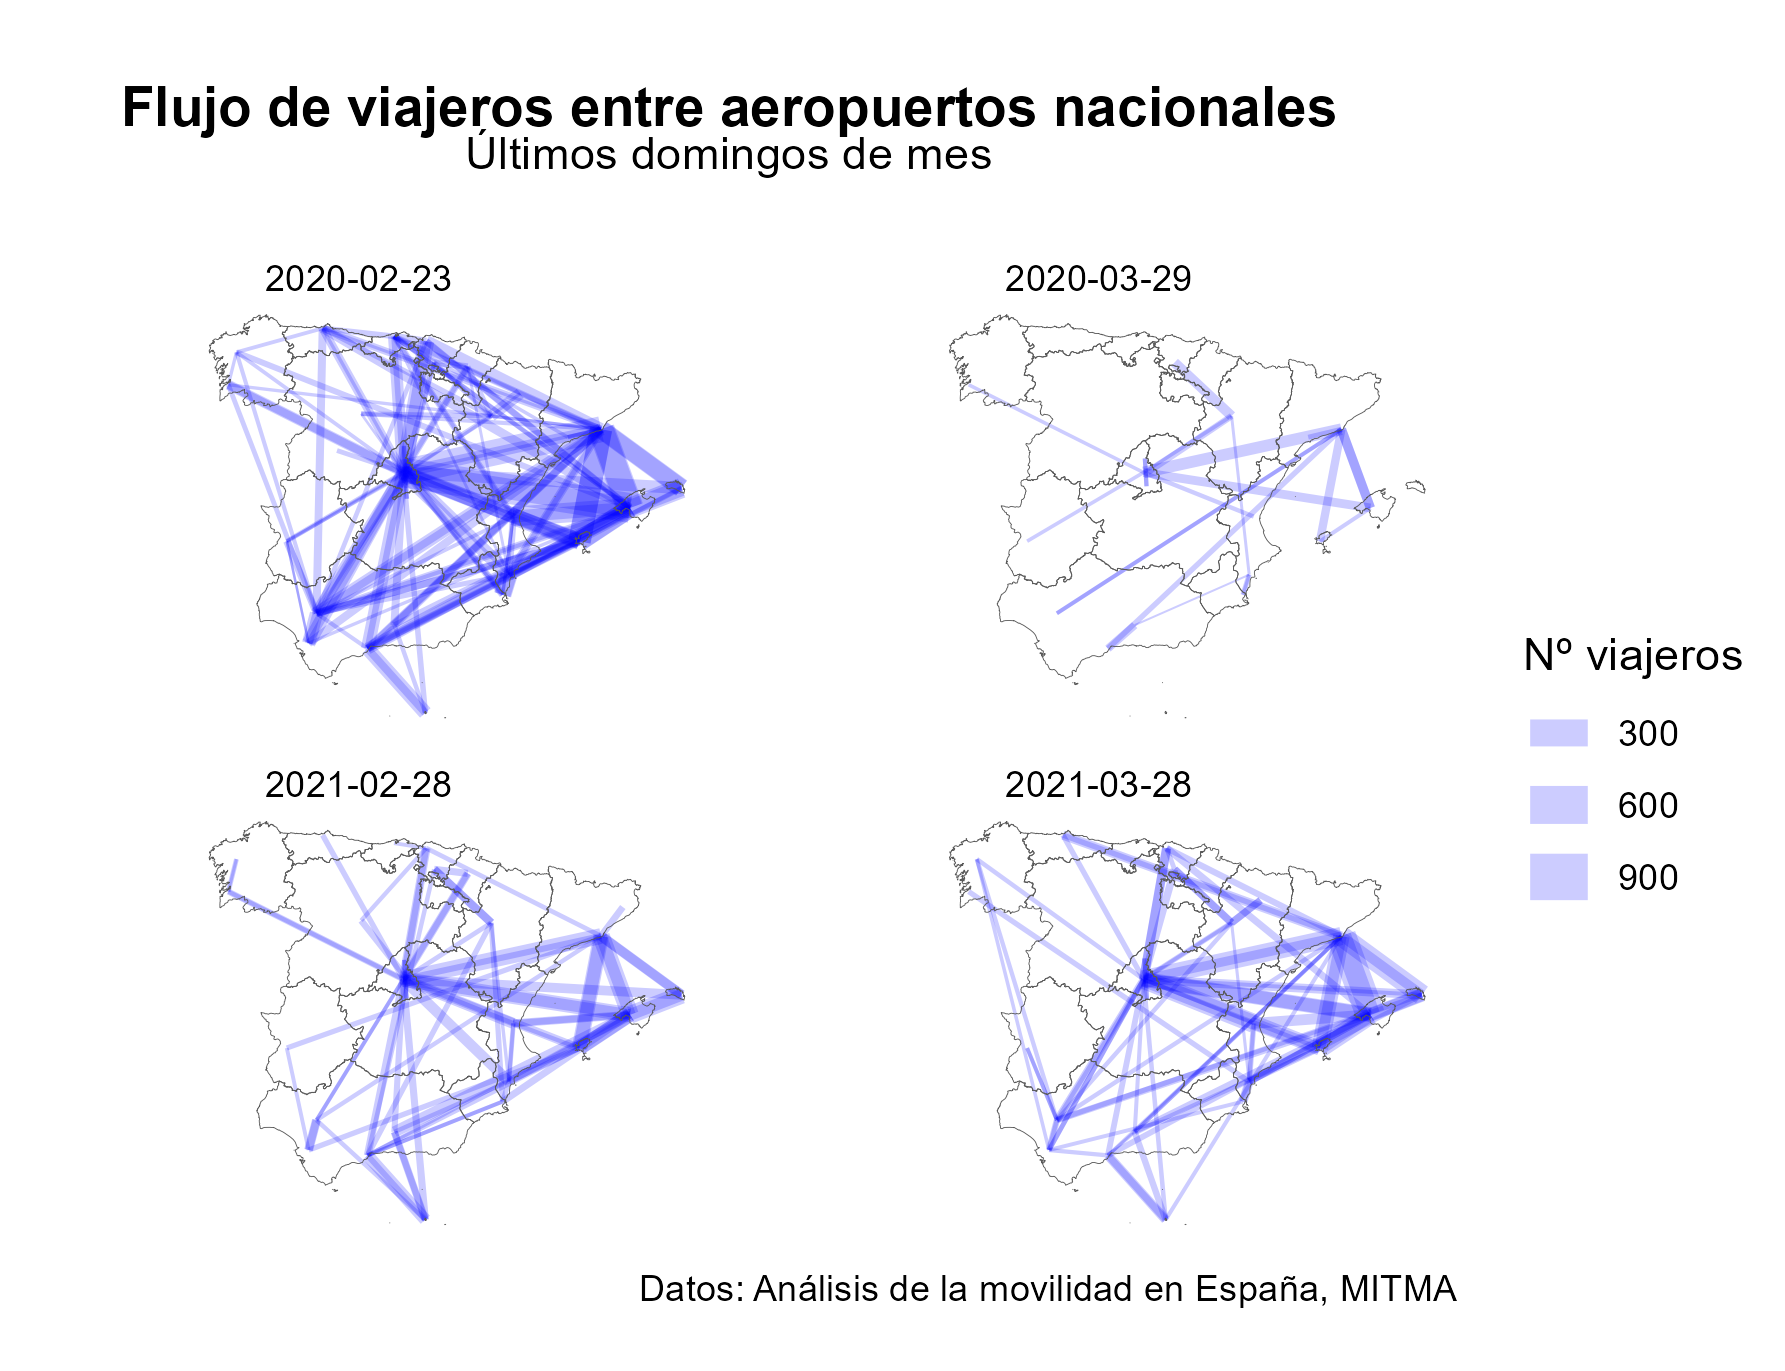
\includegraphics[width=0.6\linewidth]{img/movilidad_covid} 

}

\caption{Análisis de movilidad COVID}\label{fig:mov}
\end{figure}

\hypertarget{datos-geogruxe1ficos}{%
\chapter{Datos geográficos}\label{datos-geogruxe1ficos}}

\hypertarget{contexto-general}{%
\section{Contexto general}\label{contexto-general}}

La palabra geográfico puede dividirse en \textbf{geo} (tierra) + \textbf{gráfico}
(dibujo/mapa). Por tanto, los datos geográficos contienen información de
cualquier variable referenciada en un punto/área de la superficie terrestre y
pueden representarse en mapas. El desarrollo de los datos geográficos ha
producido grandes bases de datos espaciales y, a su vez, ha propiciado el
desarrollo de herramientas para su tratamiento como los ya mencionados Sistemas
de información geográficos y la Geocomputación.

\textbf{¿Qué hace un Sistemas de información geográfico?}

Un Sistema de información geográfica (SIG) es una herramienta que crea,
administra, analiza y mapea todo tipo de datos. GIS conecta datos a un mapa,
integrando datos de ubicación (\textbf{dónde} están las cosas) con todo tipo de
información descriptiva (\textbf{cómo} son las cosas allí).

Esto proporciona una base para el mapeo y el análisis que se utiliza en la
ciencia y en casi todas las industrias. GIS ayuda a los usuarios a comprender
patrones, relaciones y contexto geográfico. Los beneficios incluyen una mejor
comunicación y eficiencia, así como una mejor gestión y toma de decisiones.

La Fig. \ref{fig:gisflujo} muestra el flujo de trabajo de los SIG, que va desde
(i) la elaboración de mapas, (ii) la obtención de geodatos o datos espaciales,
(iii) el análisis de los datos geográficamente referenciados y (iv) la edición,
mapeo y presentación de los resultados.

\begin{figure}

{\centering 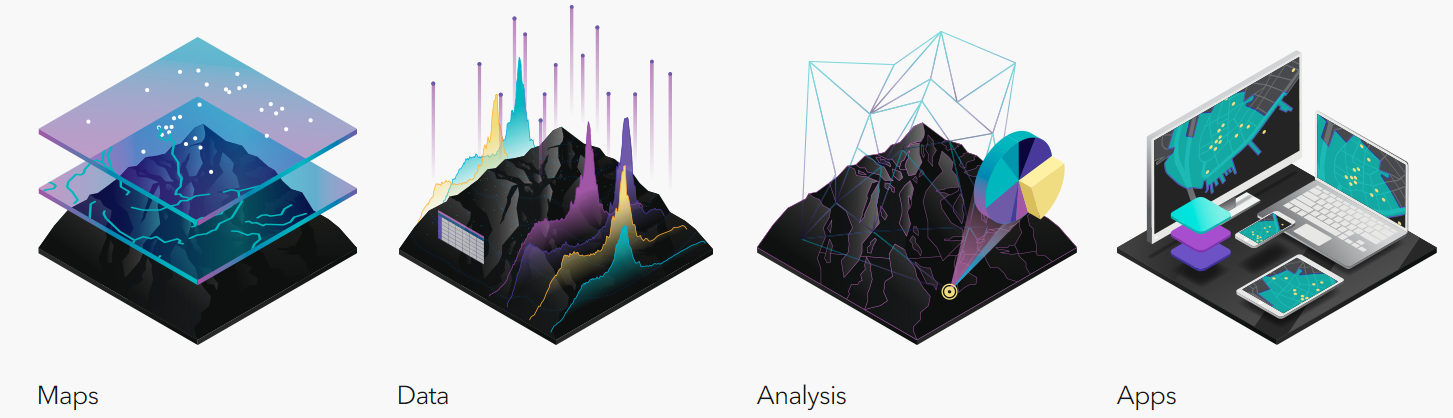
\includegraphics[width=0.7\linewidth]{img/GIS} 

}

\caption{Flujo de trabajo de los GIS. Fuente: https://www.esri.com/en-us/what-is-gis/overview}\label{fig:gisflujo}
\end{figure}

Pero es más, el desarrollo de la \textbf{Inteligencia Artificial} y la \textbf{Inteligencia
computacional} se han convertido en herramientas creativas y complementarias a
los convencionales GIS, dando origen a la \emph{Geocomputación}, que trata de
utilizar el \emph{poder de los ordenadores para hacer cosas con los datos
geográficos}.

\textbf{¿Y que es la Geocomputación?}

En primer lugar, señalar que, aunque la geocomputación es un término
relativamente nuevo se encuentra influenciado por otros términos clásicos. De
manera sencilla puede definirse como \emph{``el proceso de aplicar tecnologías de
computación a problemas geográficos''} \citep{rees1998}. \citet{Openshaw_Abrahart_2000}
aporta más elementos formales a esta definición destacando que \emph{``la
geocomputación trata sobre los diferentes tipos de geodatos, y sobre el
desarrollo de geo-herramientas relevantes en un contexto científico''}.

La geocomputación está muy relacionada con otros términos como los SIG, ya
definidos, y con diversos tipos de campos científicos, como las Geociencias, las
Ciencias atmosféricas y climáticas, la Geoinformática, la Topología, la Ecología
y las Ciencia de datos geográficos (GDS, Geographic Data Science).

Cada término comparte un énfasis en un enfoque \textbf{científico} (que implica
reproducible y falsable) influenciado por los GIS, aunque sus orígenes y
principales campos de aplicación difieren. La geocomputación es ámpliamente
utilizada en ámbitos como la sociología, el análisis político o el desarrollo de
aplicaciones para móviles. Por tanto, usamos geocomputación como un sinónimo
aproximado que encapsula a todas las ciencias que buscan usar datos geográficos
para trabajos científicos aplicados.

\textbf{¿Por que R para datos geográficos?}

R es una herramienta con capacidades avanzadas de análisis, modelado y
visualización. Por ejemplo, los nuevos entornos de desarrollo integrado (en
inglés, Integrated Development Environment, \textbf{IDE}), como RStudio, han hecho
que R sea más fácil de usar para muchos, facilitando la creación de mapas con un
panel dedicado a la visualización interactiva \citep{Lovelance_et_al_2019}. Además,
el uso del código R permite la enseñanza de la geocomputación con referencia a
ejemplos reproducibles en lugar de conceptos abstractos. Por ejemplo, de una
forma relativamente sencialla, se puede geoposicionar de manera interactiva la
localización de la Puerta del Sol en Madrid y, además, dejar la el código R para
hacerlo reproducible, ver Fig. \ref{fig:leaflet}.

\begin{Shaded}
\begin{Highlighting}[]
\FunctionTok{library}\NormalTok{(leaflet)}
\FunctionTok{leaflet}\NormalTok{(}\AttributeTok{width =} \StringTok{"100\%"}\NormalTok{, }\AttributeTok{height =} \StringTok{"500px"}\NormalTok{) }\SpecialCharTok{\%\textgreater{}\%}
  \FunctionTok{addTiles}\NormalTok{() }\SpecialCharTok{\%\textgreater{}\%}
  \FunctionTok{setView}\NormalTok{(}\SpecialCharTok{{-}}\FloatTok{3.703548}\NormalTok{, }\FloatTok{40.417147}\NormalTok{, }\AttributeTok{zoom =} \DecValTok{60}\NormalTok{)}
\end{Highlighting}
\end{Shaded}

\begin{figure}

{\centering 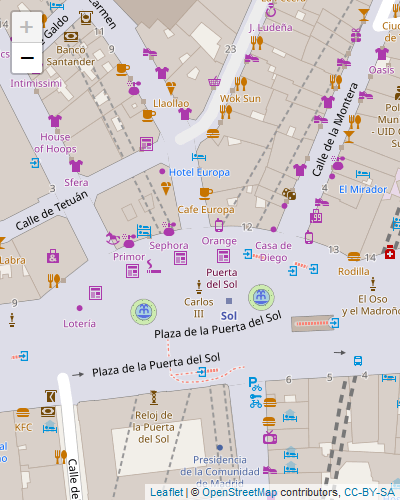
\includegraphics[width=0.6\linewidth]{_main_files/figure-latex/leaflet-1} 

}

\caption{Localización interactiva de la Puerta del Sol en Madrid}\label{fig:leaflet}
\end{figure}

Por otra parte R dispone de cientos de librerías especializadas para datos
espaciales. Una descripción detallada puede ver se en \href{https://cran.r-project.org/web/views/Spatial.html}{CRAN Task View: Analysis
of Spatial Data}

Para no abrumar al lector, a continuación se muestran, de manera esquemática,
las librerías más usadas para el tratamiento de datos espaciales y que se
emplearán a lo largo de la asignatura Estadística Espacial y Espacio-Temporal,
no sólo en el tema que nos ocupa:

\begin{itemize}
\item
  \texttt{sp} y \texttt{sf}: para el tratamiento de clases y métodos de los datos
  vectoriales.
\item
  \texttt{raster},\texttt{terra} y \texttt{stars} para datos raster.
\item
  \texttt{gstat} y \texttt{geoR}: para el análisis de datos geoestadísticos, ajuste y
  estimación de semivariogramas, interpolación, etc.
\item
  \texttt{spdep} para el análisis de datos con modelos de econometría espacial,
  creación de matrices de contiguidad/distancia \textbf{W}, estimación de modelos
  econométricos espaciales, etc
\item
  \texttt{spatstat} para el análisis de procesos de puntos espaciales, intensidad,
  etc.
\end{itemize}

\hypertarget{conceptos-clave}{%
\section{Conceptos clave}\label{conceptos-clave}}

Una vez visto el contexto actual de los datos georreferenciados y antes de
entrar en detalle en su análisis, debemos tener en cuenta una serie de conceptos
clave que se irán desarrollando a lo largo del tema.

Hemos dicho que Geográfico = Geo (tierra) + gráfico (mapa). Por tanto, si
tenemos varios datos geográficos, localizados en distintos puntos de la tierra,
es porque tenemos las \textbf{coordenadas} que los posicionan en esos puntos
concretos. Asociado a estas coordenadas debemos conocer el \textbf{Sistema de
referencia de espacial} o Coordinate reference system (CRS) en el que están
proyectadas dichas coordenadas.

Por otra parte, los formatos de estos datos pueden ser \textbf{vectores} o \textbf{raster}
como se explicará en la Sección \ref{formatos}.

Si damos un paso más e incorporamos el concepto de \textbf{distancia}, pues es lógico
pensar que en un fenómeno de interés, por ejemplo, la modelización de la
cantidad y dirección de lava en La Palma tras la erupción del volcán ``Cumbre
Vieja'', la distancia es un factor clave, pues aquellas zonas más cercanas al
volcán tendrán niveles más parecidos entre sí y con valores más altos que
aquellas que están más alejadas

En este caso el nivel de contaminación en el aire en La Palma no puede ser
modelado como si las observaciones fuesen independientes pues las más cercanas
entre sí serán más parecidas que las más lejanas, dando lugar al concepto de
\textbf{dependencia espacial}. Y depende del tipo de datos espaciales tendremos tres
grandes formas de abordar el tratamiento de los datos espaciales:
\textbf{geoestadística}, \textbf{procesos de punto} y \textbf{econometría espacial} (véase
sección \ref{CRS}).

\begin{figure}

{\centering 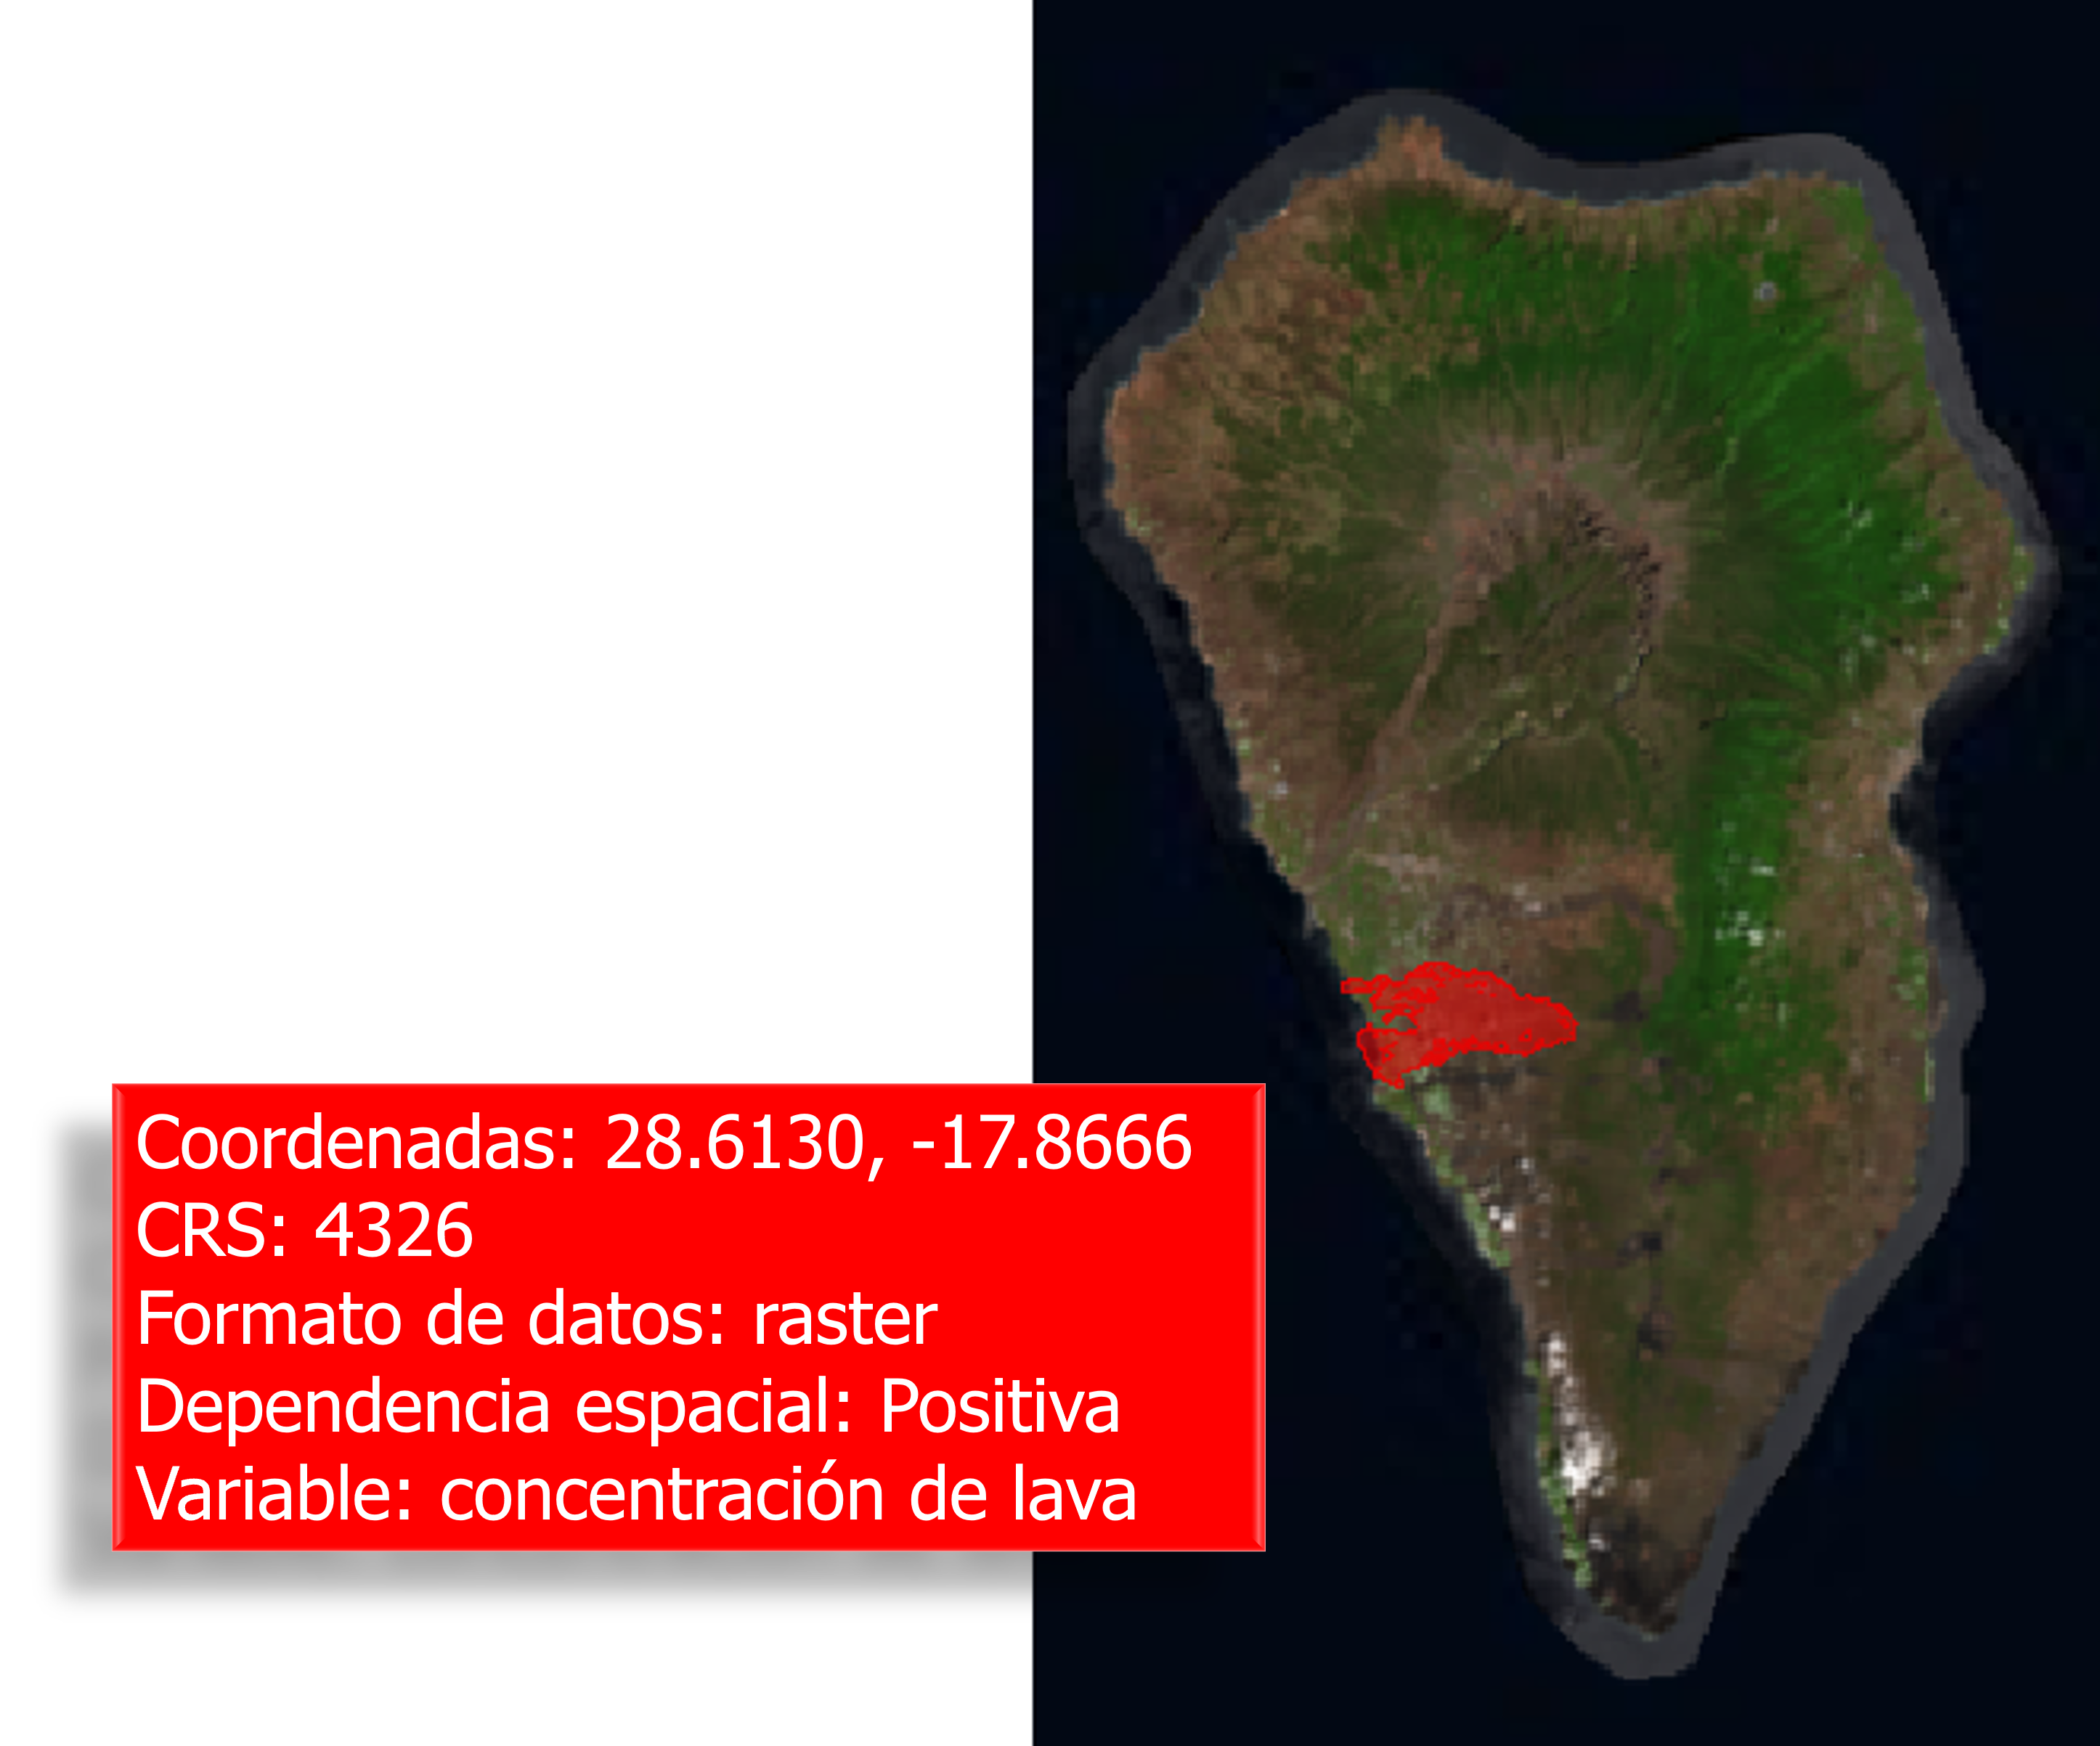
\includegraphics[width=0.6\linewidth]{img/Cumbrevieja} 

}

\caption{Información espacial de la concentración de lava en Cumbre Vieja}\label{fig:gis}
\end{figure}

\hypertarget{formatos}{%
\chapter{Formatos de datos espaciales}\label{formatos}}

\hypertarget{tipos-de-ficheros-completar}{%
\section{Tipos de ficheros (COMPLETAR)}\label{tipos-de-ficheros-completar}}

Poner el esquema de los Shapes.

\url{https://en.wikipedia.org/wiki/Shapefile}

Yo no sé, DIEGO, si en gisco R tienes la definición y lo ponemos de ahí.

Y pensar si tiene que venir aquí o dónde\ldots{} quizá al final de la sección
FORMATOS DE DATOS ESPACIALES

En el ámbito del análisis espacial en \textbf{R}, se pueden clasificar \textbf{el formato}
de datos espaciales en función del modelo de datos \citep{Lovelance_et_al_2019}. Se
pueden distinguir dos tipos de modelos de datos: vectores y raster.

\hypertarget{datos-de-vectores}{%
\section{Datos de vectores}\label{datos-de-vectores}}

Este modelo está basado en puntos georeferenciados. Los \textbf{puntos} pueden
representar localizaciones específicas, como la localización de edificios:

\begin{Shaded}
\begin{Highlighting}[]

\FunctionTok{library}\NormalTok{(ggplot2)}
\FunctionTok{library}\NormalTok{(sf)}


\CommentTok{\# Hospitales en Toledo segun Eurostat}
\NormalTok{hosp\_toledo }\OtherTok{\textless{}{-}} \FunctionTok{st\_read}\NormalTok{(}\StringTok{"data/hosp\_toledo.geojson"}\NormalTok{, }\AttributeTok{quiet =} \ConstantTok{TRUE}\NormalTok{)}

\CommentTok{\# Plot}
\FunctionTok{ggplot}\NormalTok{() }\SpecialCharTok{+}
  \FunctionTok{geom\_sf}\NormalTok{(}
    \AttributeTok{data =}\NormalTok{ hosp\_toledo, }\FunctionTok{aes}\NormalTok{(}\AttributeTok{fill =} \StringTok{"Centros Sanitarios"}\NormalTok{),}
    \AttributeTok{color =} \StringTok{"blue"}
\NormalTok{  ) }\SpecialCharTok{+}
  \FunctionTok{labs}\NormalTok{(}
    \AttributeTok{caption =} \StringTok{"Datos: Eurostat"}\NormalTok{,}
    \AttributeTok{title =} \StringTok{"Hospitales y Centros de Salud en Toledo"}\NormalTok{,}
    \AttributeTok{fill =} \StringTok{""}
\NormalTok{  ) }\SpecialCharTok{+}
  \FunctionTok{theme\_minimal}\NormalTok{() }\SpecialCharTok{+}
  \FunctionTok{theme}\NormalTok{(}\AttributeTok{legend.position =} \StringTok{"bottom"}\NormalTok{)}
\end{Highlighting}
\end{Shaded}

\begin{figure}

{\centering 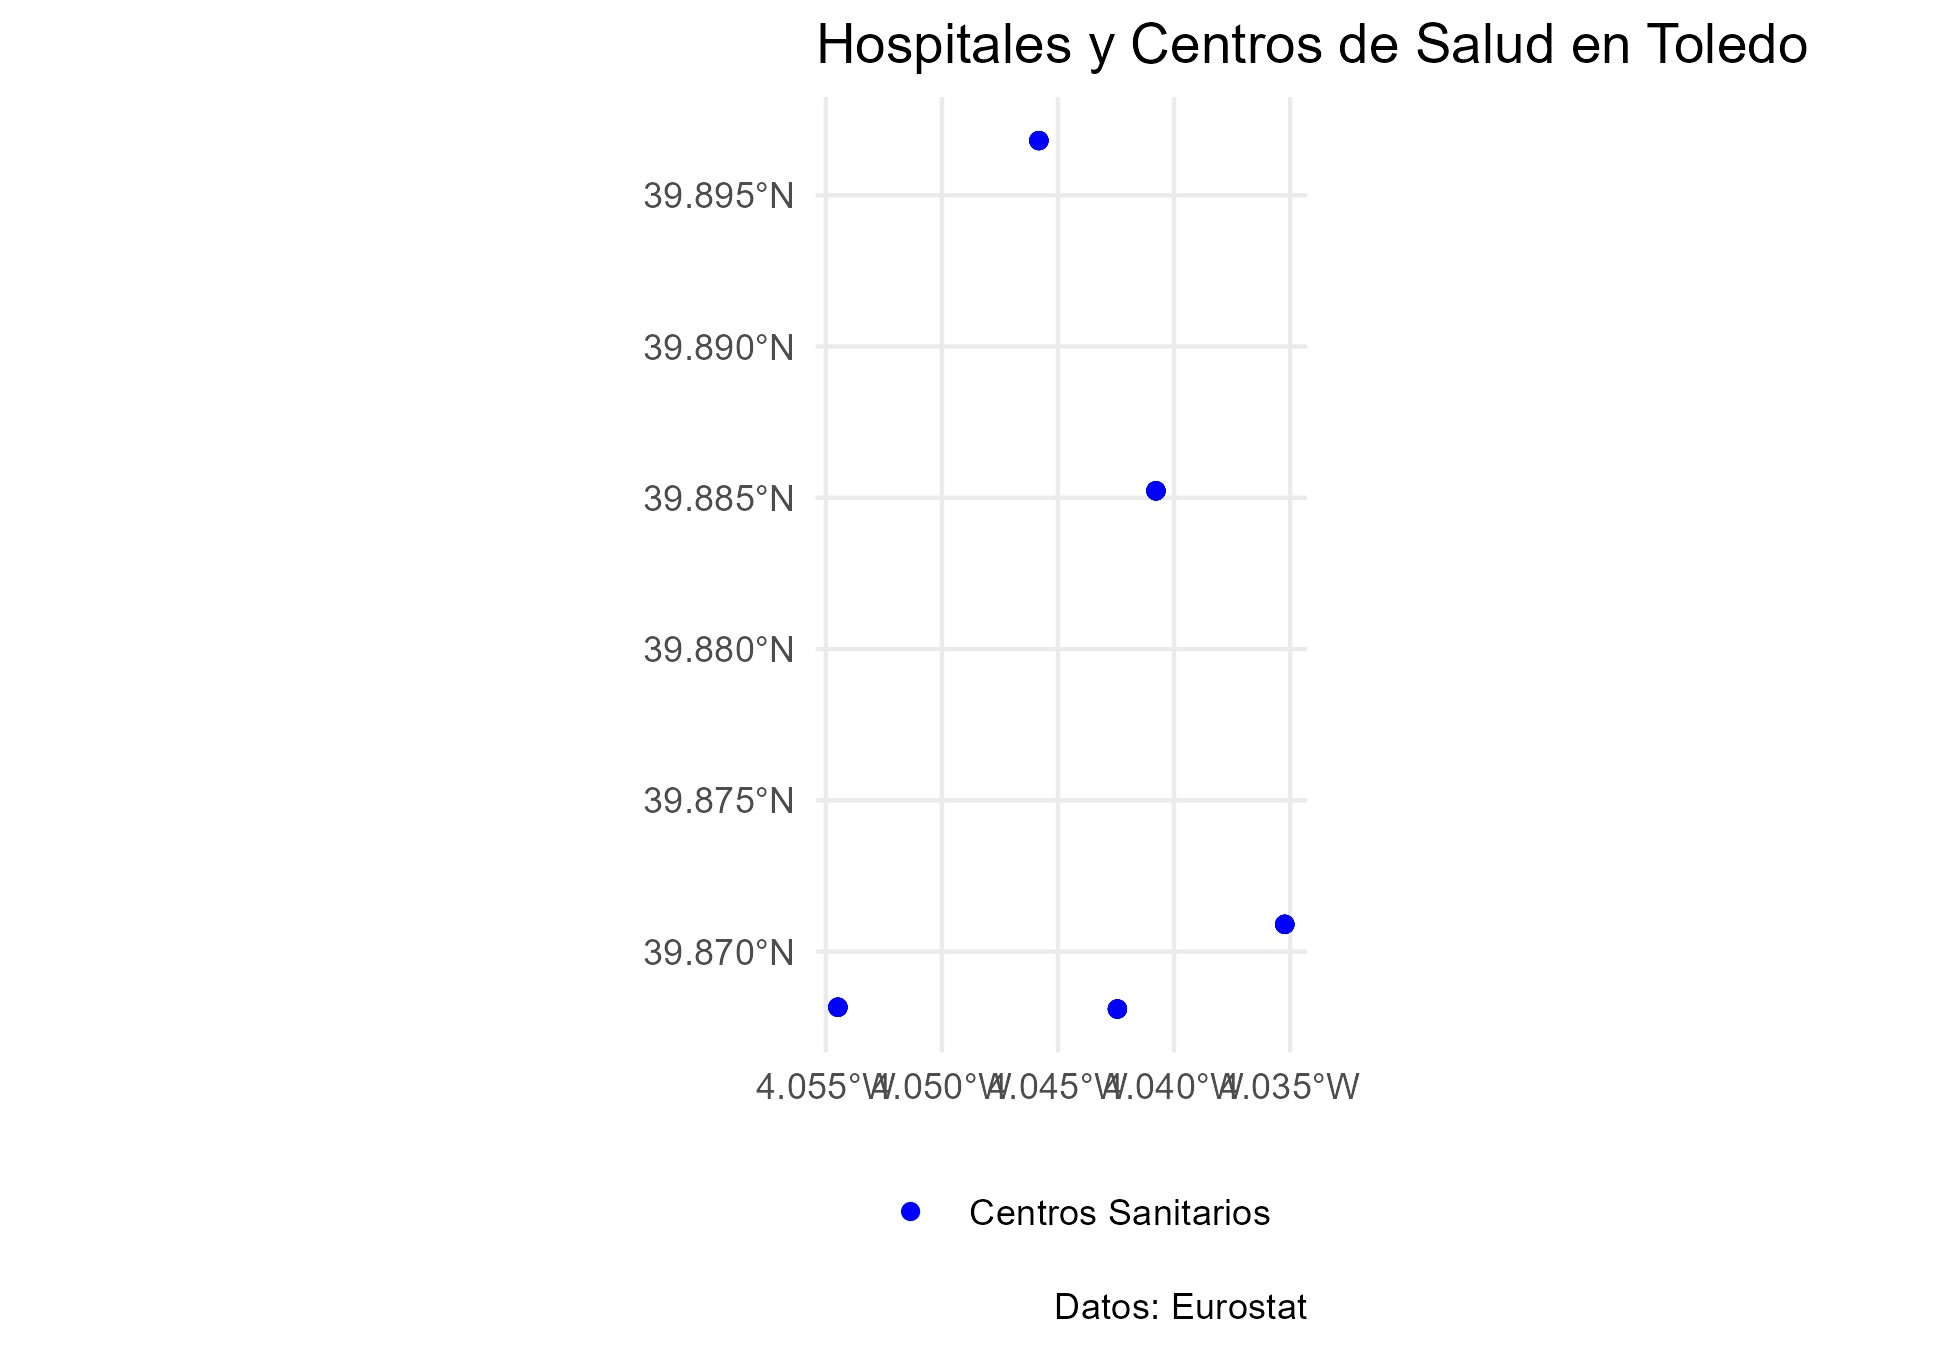
\includegraphics[width=0.6\linewidth]{_main_files/figure-latex/puntos-1} 

}

\caption{Datos vector: Puntos}\label{fig:puntos}
\end{figure}

Estos puntos también pueden estar conectados entre sí, de manera que formen
geometrías más complejas, como \textbf{líneas} y \textbf{polígonos}:

\begin{Shaded}
\begin{Highlighting}[]

\NormalTok{tajo }\OtherTok{\textless{}{-}} \FunctionTok{st\_read}\NormalTok{(}\StringTok{"data/tajo\_toledo.shp"}\NormalTok{, }\AttributeTok{quiet =} \ConstantTok{TRUE}\NormalTok{)}
\NormalTok{toledo }\OtherTok{\textless{}{-}} \FunctionTok{st\_read}\NormalTok{(}\StringTok{"data/toledo\_ciudad.gpkg"}\NormalTok{, }\AttributeTok{quiet =} \ConstantTok{TRUE}\NormalTok{)}


\FunctionTok{ggplot}\NormalTok{(toledo) }\SpecialCharTok{+}
  \FunctionTok{geom\_sf}\NormalTok{(}\AttributeTok{fill =} \StringTok{"cornsilk2"}\NormalTok{) }\SpecialCharTok{+}
  \FunctionTok{geom\_sf}\NormalTok{(}\AttributeTok{data =}\NormalTok{ tajo, }\AttributeTok{col =} \StringTok{"lightblue2"}\NormalTok{, }\AttributeTok{lwd =} \DecValTok{2}\NormalTok{, }\AttributeTok{alpha =} \FloatTok{0.7}\NormalTok{) }\SpecialCharTok{+}
  \FunctionTok{geom\_sf}\NormalTok{(}\AttributeTok{data =}\NormalTok{ hosp\_toledo, }\AttributeTok{col =} \StringTok{"blue"}\NormalTok{) }\SpecialCharTok{+}
  \FunctionTok{coord\_sf}\NormalTok{(}
    \AttributeTok{xlim =} \FunctionTok{c}\NormalTok{(}\SpecialCharTok{{-}}\FloatTok{4.2}\NormalTok{, }\SpecialCharTok{{-}}\FloatTok{3.8}\NormalTok{),}
    \AttributeTok{ylim =} \FunctionTok{c}\NormalTok{(}\FloatTok{39.8}\NormalTok{, }\FloatTok{39.95}\NormalTok{)}
\NormalTok{  ) }\SpecialCharTok{+}
  \FunctionTok{theme\_minimal}\NormalTok{()}
\end{Highlighting}
\end{Shaded}

\begin{figure}

{\centering 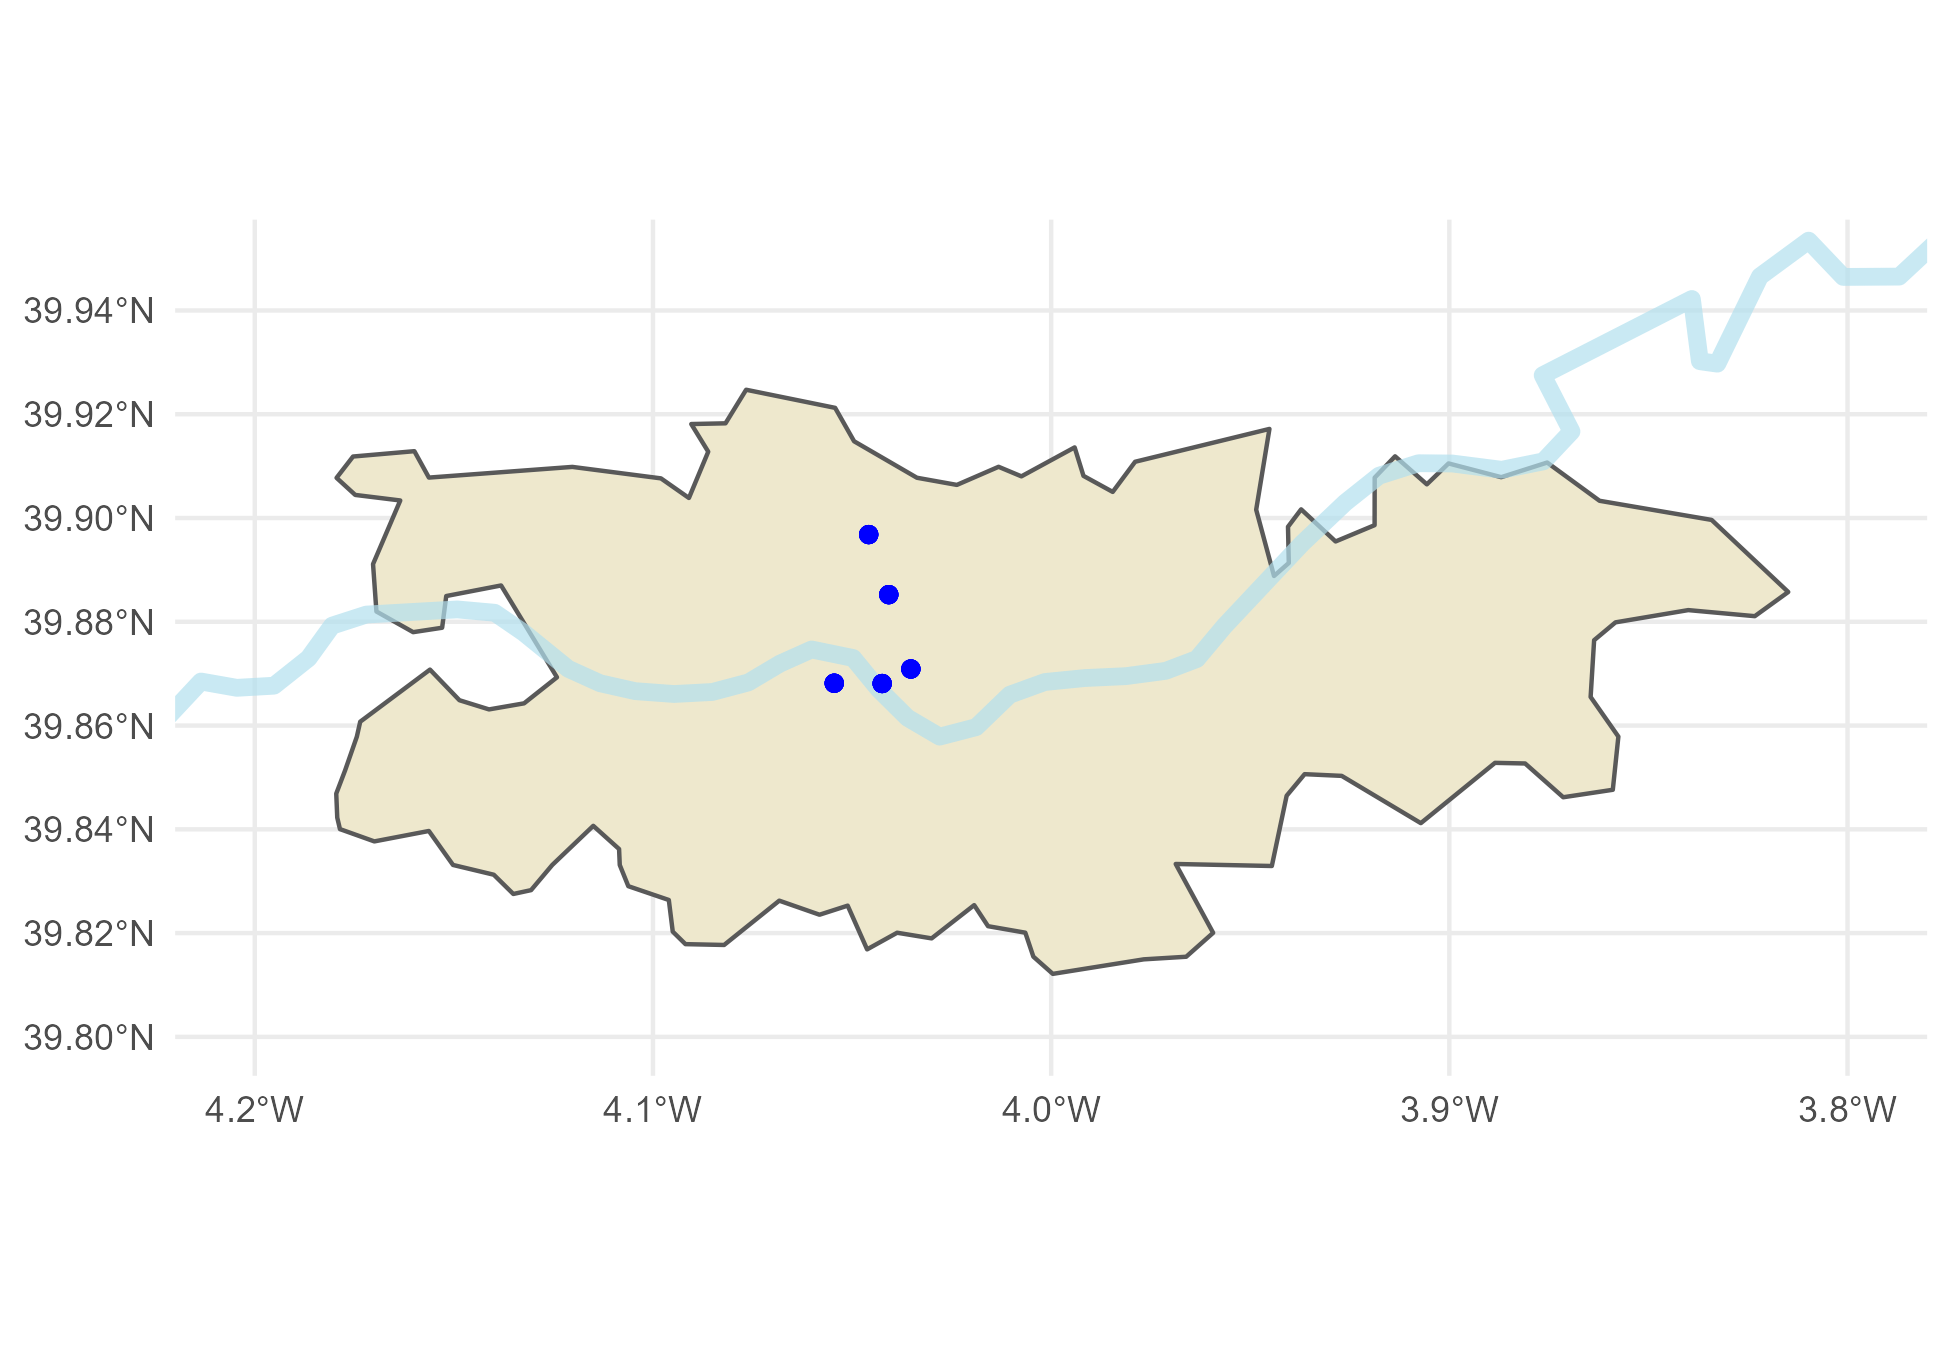
\includegraphics[width=0.6\linewidth]{_main_files/figure-latex/lineas-pol-1} 

}

\caption{Datos vector: Puntos, líneas y polígonos}\label{fig:lineas-pol}
\end{figure}

En la Fig. \ref{fig:lineas-pol}, el río Tajo está representado como una línea
(sucesión de puntos unidos entre sí) y la ciudad de Toledo como un polígono
(línea de puntos cerrada formando un continuo). A modo ilustrativo, la Fig.
\ref{fig:lineas-pol-desc} representa la descomposición en puntos de todos los
datos espaciales representados en la Fig. \ref{fig:lineas-pol}.

\begin{figure}

{\centering 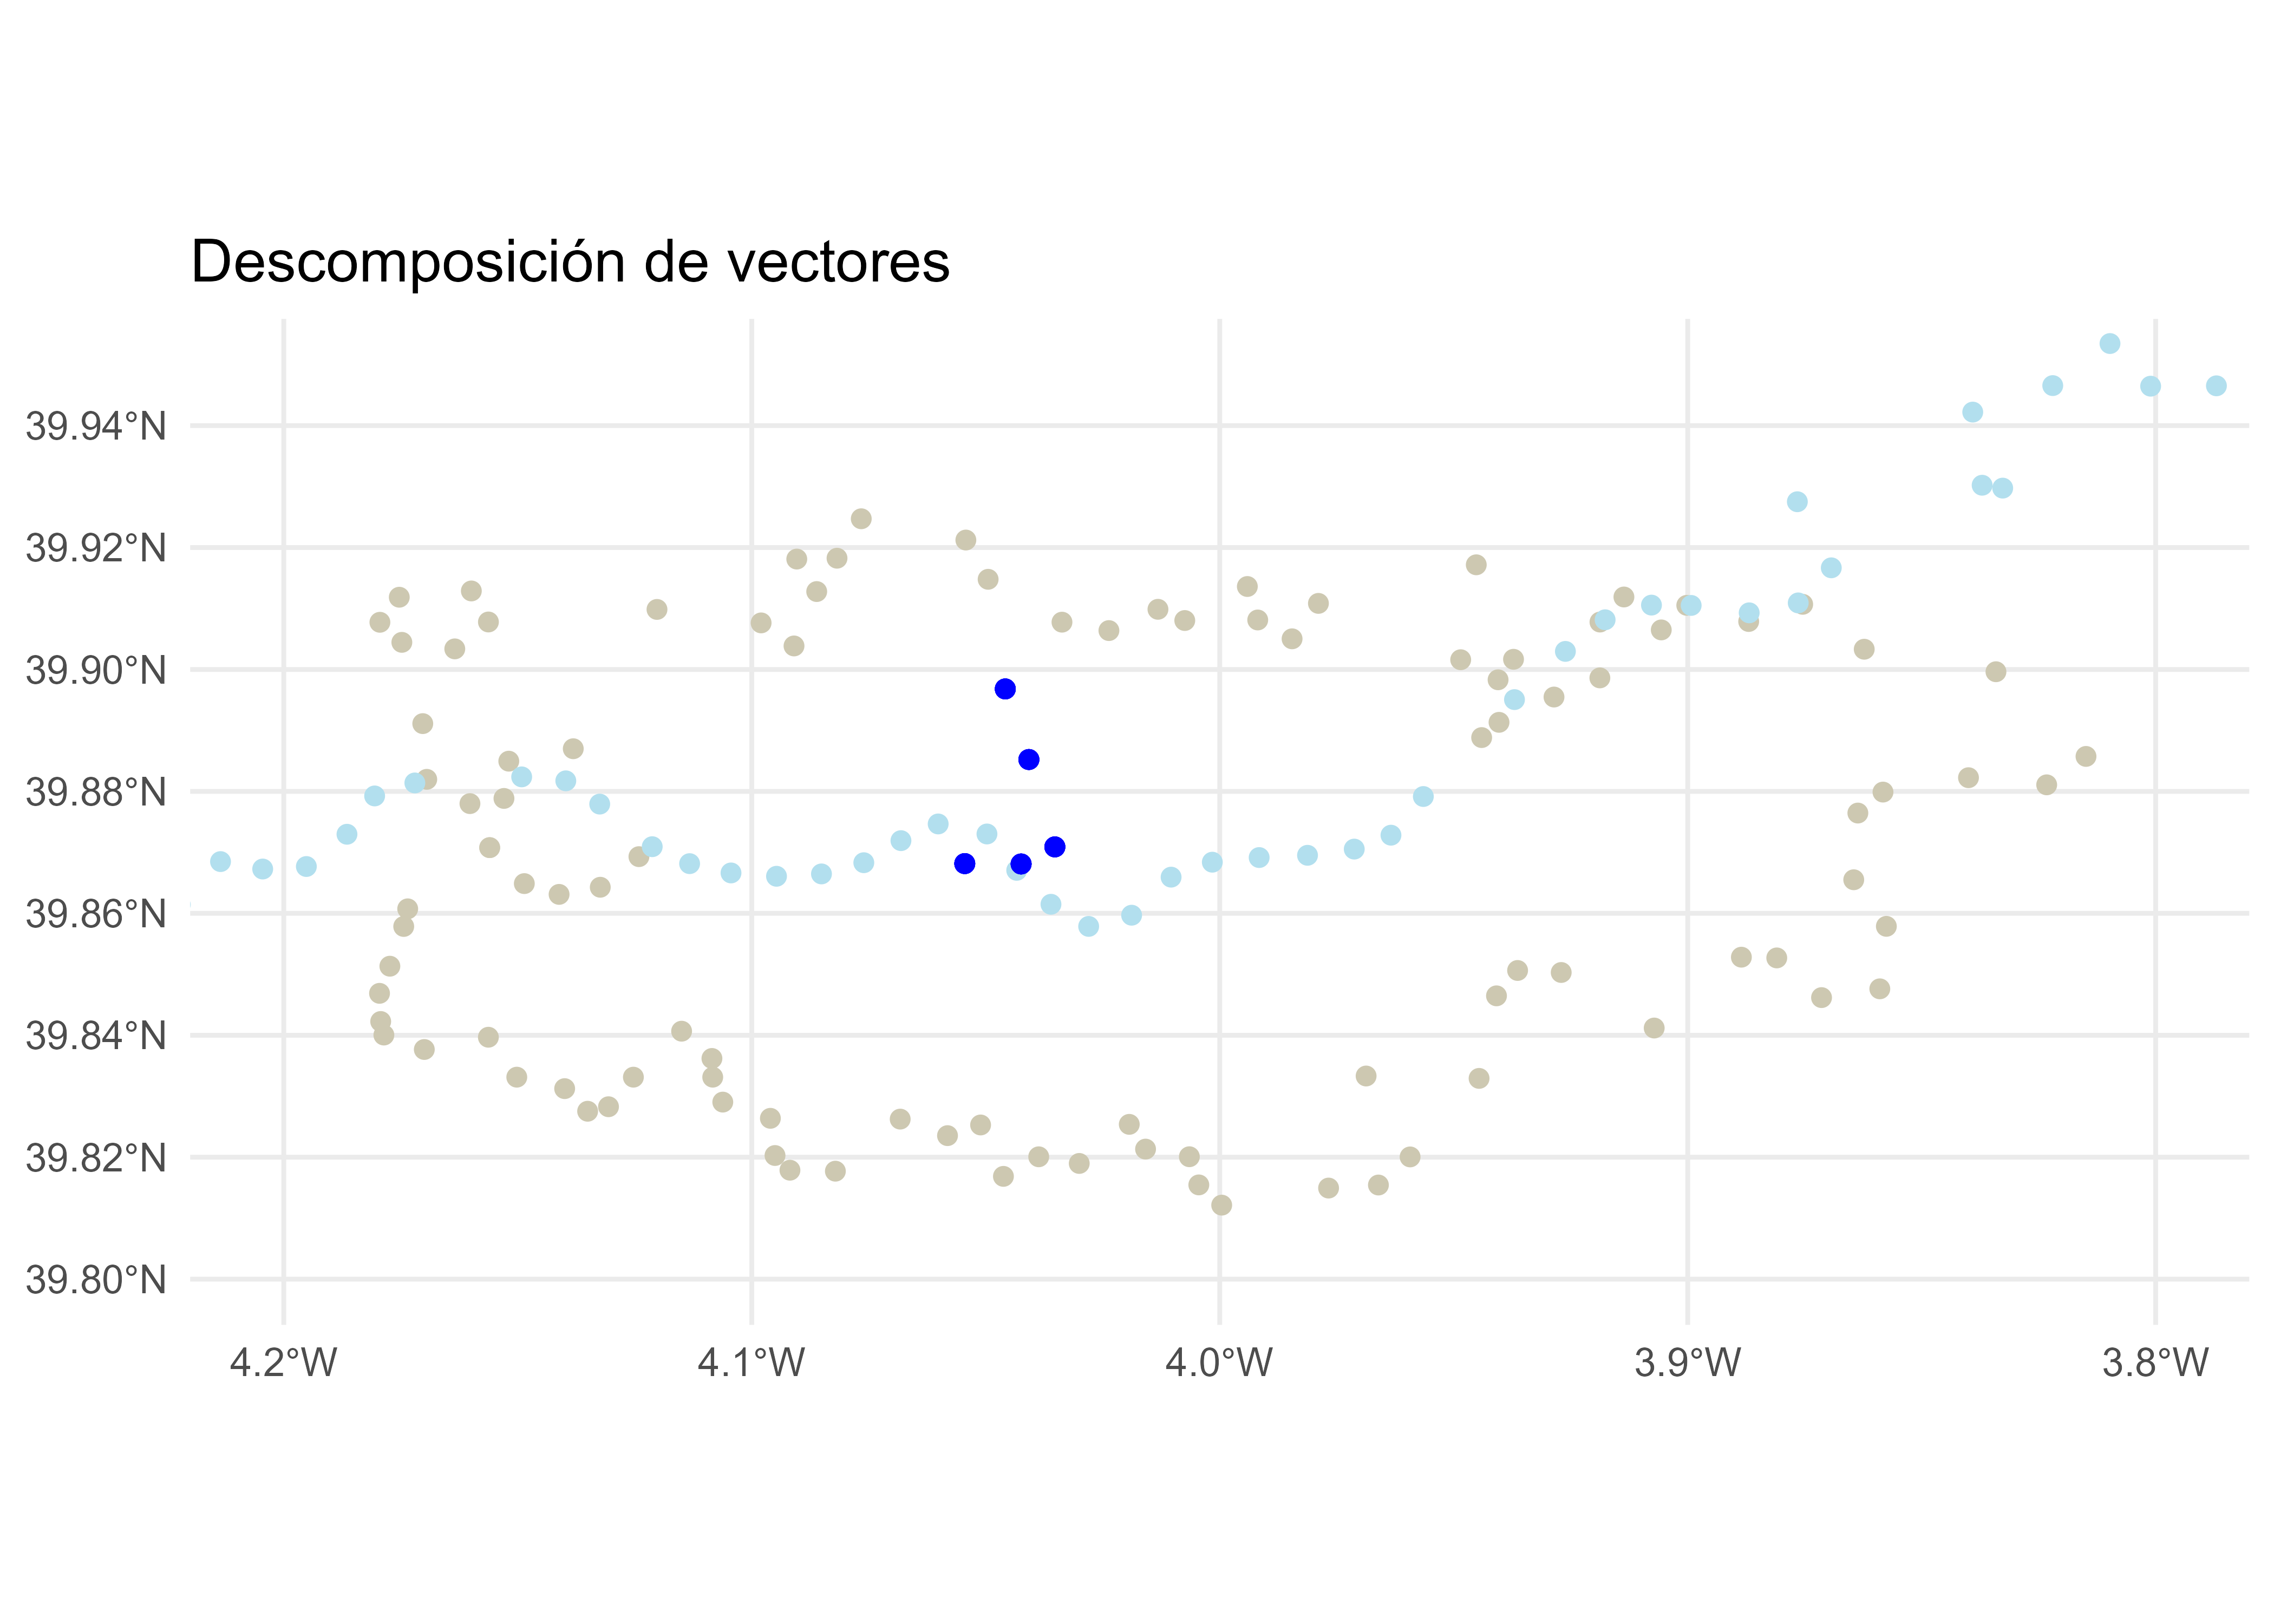
\includegraphics[width=0.6\linewidth]{_main_files/figure-latex/lineas-pol-desc-1} 

}

\caption{Datos vector: Descomposición en puntos}\label{fig:lineas-pol-desc}
\end{figure}

\hypertarget{datos-raster}{%
\section{Datos raster}\label{datos-raster}}

Los datos ráster son datos representandos en una rejilla rectangular de píxeles
(denomindada \textbf{matriz}) que se puede visualizar en diversos dispositivo de
representación. El caso más cotidiano de un ráster es una fotografía, donde la
imagen se representa como una serie de celdas, determinadas por la resolución de
la imagen (número total de píxeles, determinados como número de píxeles en cada
fila por número de píxeles en cada columna) y el color que presenta cada uno de
estos píxeles.

En el ámbito de los datos espaciales, la definición es muy similar. Un archivo
ráster está formado por una malla regular de píxeles georreferenciada, tal y
como muestra la Fig. \ref{fig:raster}:

\begin{Shaded}
\begin{Highlighting}[]

\FunctionTok{library}\NormalTok{(raster)}

\NormalTok{elev }\OtherTok{\textless{}{-}} \FunctionTok{raster}\NormalTok{(}\StringTok{"data/Toledo\_DEM.tiff"}\NormalTok{)}
\FunctionTok{plot}\NormalTok{(elev, }\AttributeTok{main =} \StringTok{"Elevación de la provincia de Toledo"}\NormalTok{)}

\CommentTok{\# Mostramos el grid}
\NormalTok{pols }\OtherTok{\textless{}{-}} \FunctionTok{rasterToPolygons}\NormalTok{(elev)}
\FunctionTok{plot}\NormalTok{(pols, }\AttributeTok{add =} \ConstantTok{TRUE}\NormalTok{, }\AttributeTok{border =} \StringTok{"grey90"}\NormalTok{)}

\CommentTok{\# Añadimos la provincia}
\NormalTok{Tol\_prov }\OtherTok{\textless{}{-}} \FunctionTok{st\_read}\NormalTok{(}\StringTok{"data/Toledo\_prov.gpkg"}\NormalTok{, }\AttributeTok{quiet =} \ConstantTok{TRUE}\NormalTok{)}

\CommentTok{\# Si queremos solamente la forma en sf, usamos st\_geometry}
\FunctionTok{plot}\NormalTok{(}\FunctionTok{st\_geometry}\NormalTok{(Tol\_prov), }\AttributeTok{add =} \ConstantTok{TRUE}\NormalTok{)}
\end{Highlighting}
\end{Shaded}

\begin{figure}

{\centering 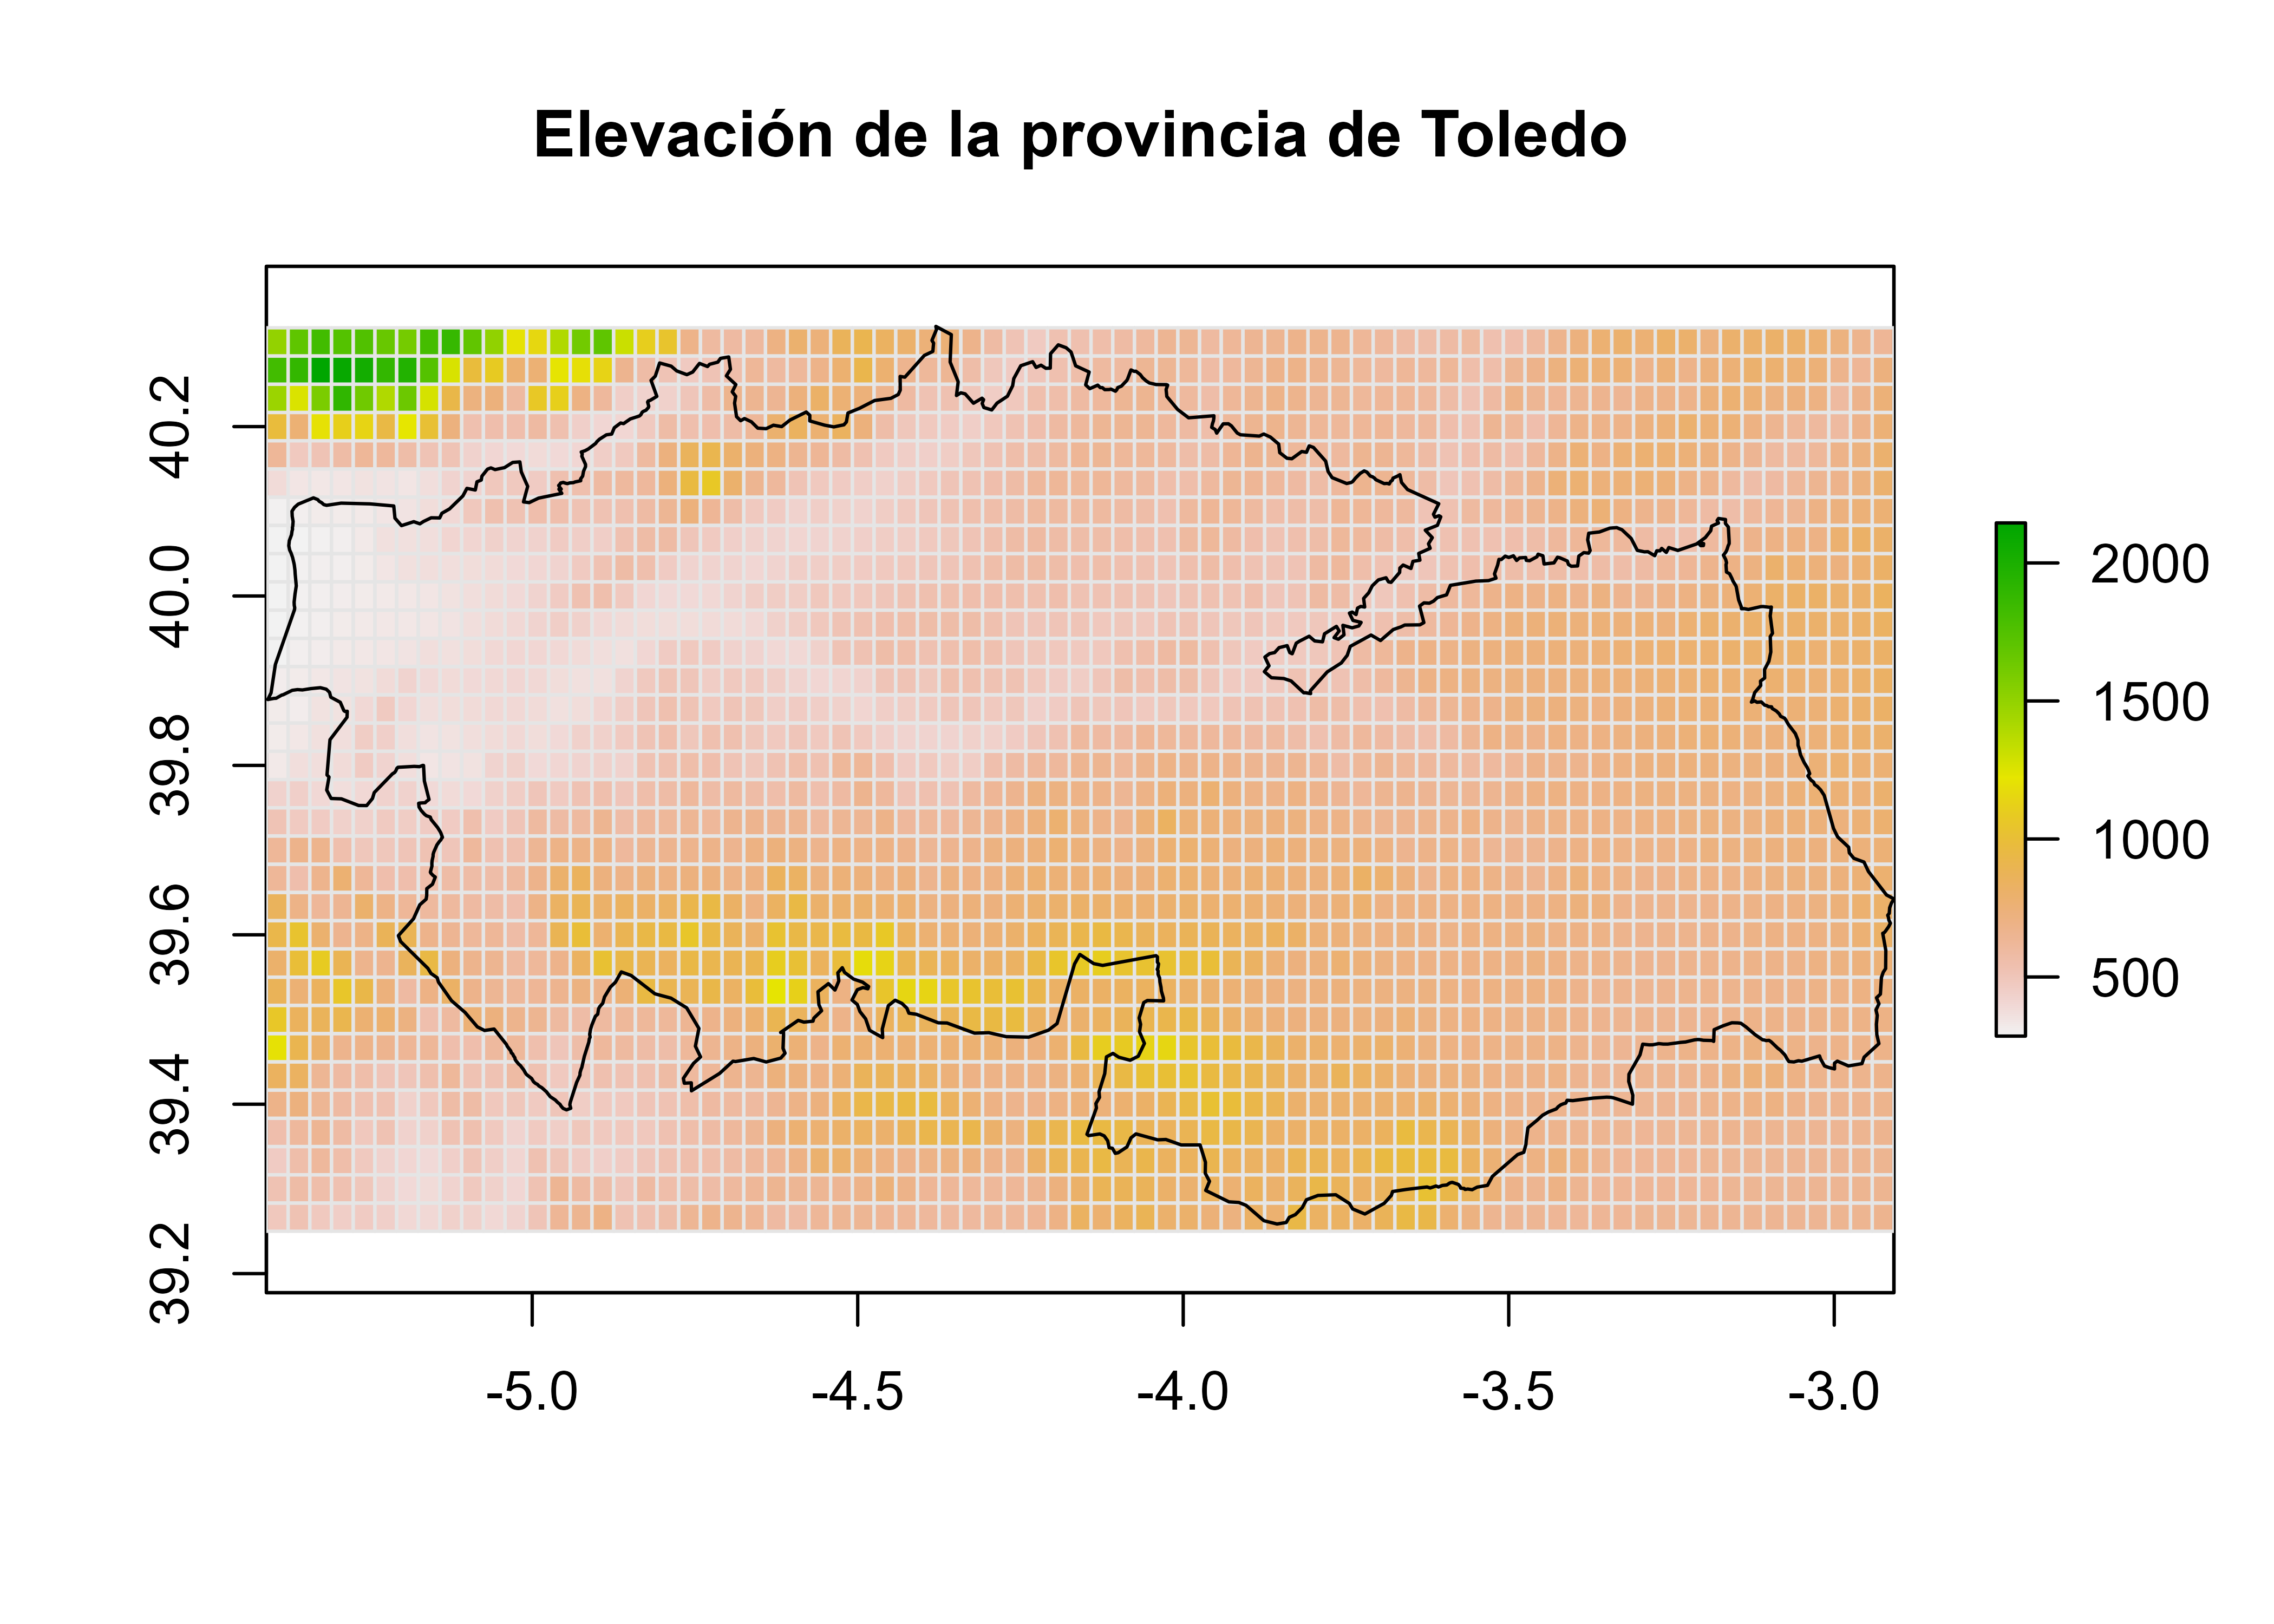
\includegraphics[width=0.6\linewidth]{_main_files/figure-latex/raster-1} 

}

\caption{Datos ráster}\label{fig:raster}
\end{figure}

En la Fig. \ref{fig:raster}, el objeto ráster \texttt{elev} tiene únicamente una capa
(denominada \texttt{ESP\_alt}). Eso implica que cada píxel tiene asociado un único
valor, en este caso, en este caso la altitud media del terreno observada:

\begin{table}

\caption{\label{tab:detalle-pixel}Datos de un ráster (detalle)}
\centering
\begin{tabular}[t]{r|r|r}
\hline
x & y & Toledo\_DEM\\
\hline
-5.391667 & 40.3 & 1498.312\\
\hline
-5.358333 & 40.3 & 1701.125\\
\hline
-5.325000 & 40.3 & 1825.312\\
\hline
-5.291667 & 40.3 & 1739.062\\
\hline
-5.258333 & 40.3 & 1756.062\\
\hline
-5.225000 & 40.3 & 1659.688\\
\hline
-5.191667 & 40.3 & 1607.375\\
\hline
-5.158333 & 40.3 & 1809.562\\
\hline
-5.125000 & 40.3 & 1874.625\\
\hline
-5.091667 & 40.3 & 1691.312\\
\hline
-5.058333 & 40.3 & 1511.500\\
\hline
-5.025000 & 40.3 & 1207.000\\
\hline
-4.991667 & 40.3 & 1160.125\\
\hline
-4.958333 & 40.3 & 1396.125\\
\hline
-4.925000 & 40.3 & 1624.125\\
\hline
\end{tabular}
\end{table}

\begin{figure}

{\centering 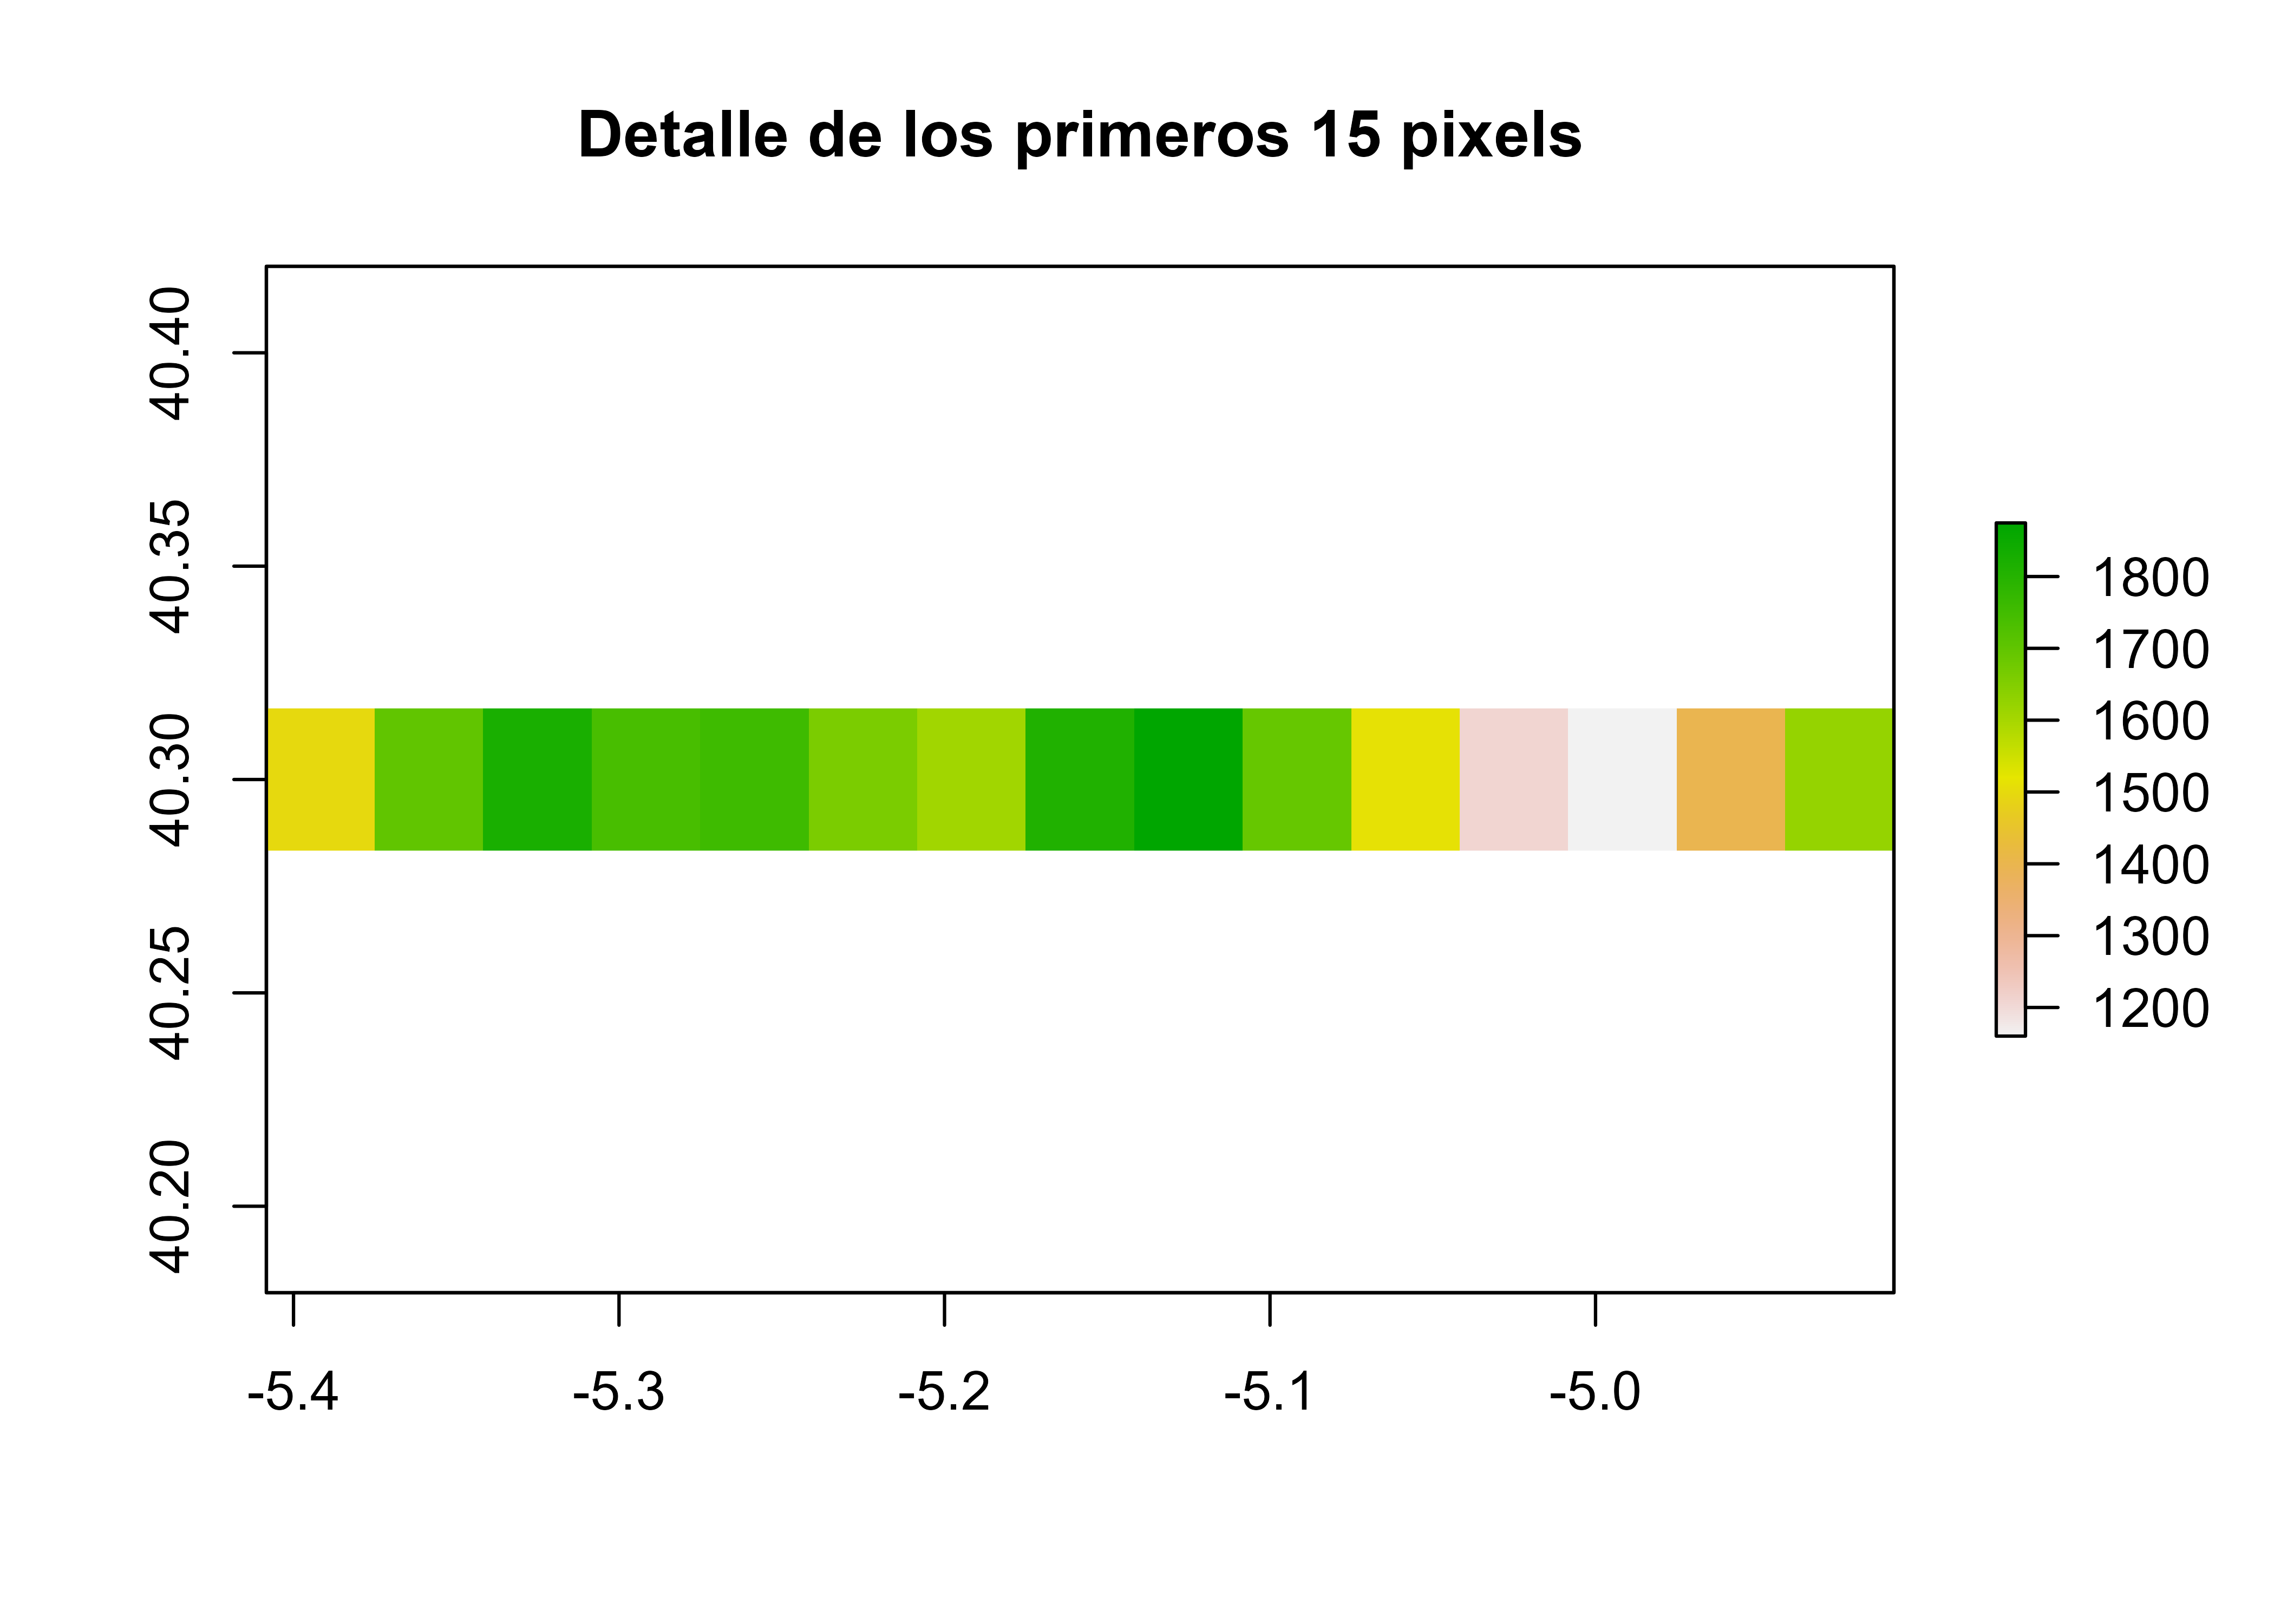
\includegraphics[width=0.6\linewidth]{_main_files/figure-latex/detalle-pixel-1} 

}

\caption{Datos ráster: Detalle}\label{fig:detalle-pixel}
\end{figure}

Los rásters pueden contener varias capas (o layers), de manera que cada píxel
puede tener asociados varios valores. Volviendo al ejemplo de la fotografía, en
un modelo simple de color RGB cada píxel lleva asociado 3 valores (rojo, verde o
azul), de manera que al combinar las tres capas se puede definir un color
distinto en cada píxel.

En la Fig. \ref{fig:raster-multilayer} vamos a usar una imagen de mapa
georreferenciada, como las proporcionadas por servicios de mapas online, para
analizar su composición.

\begin{figure}

{\centering 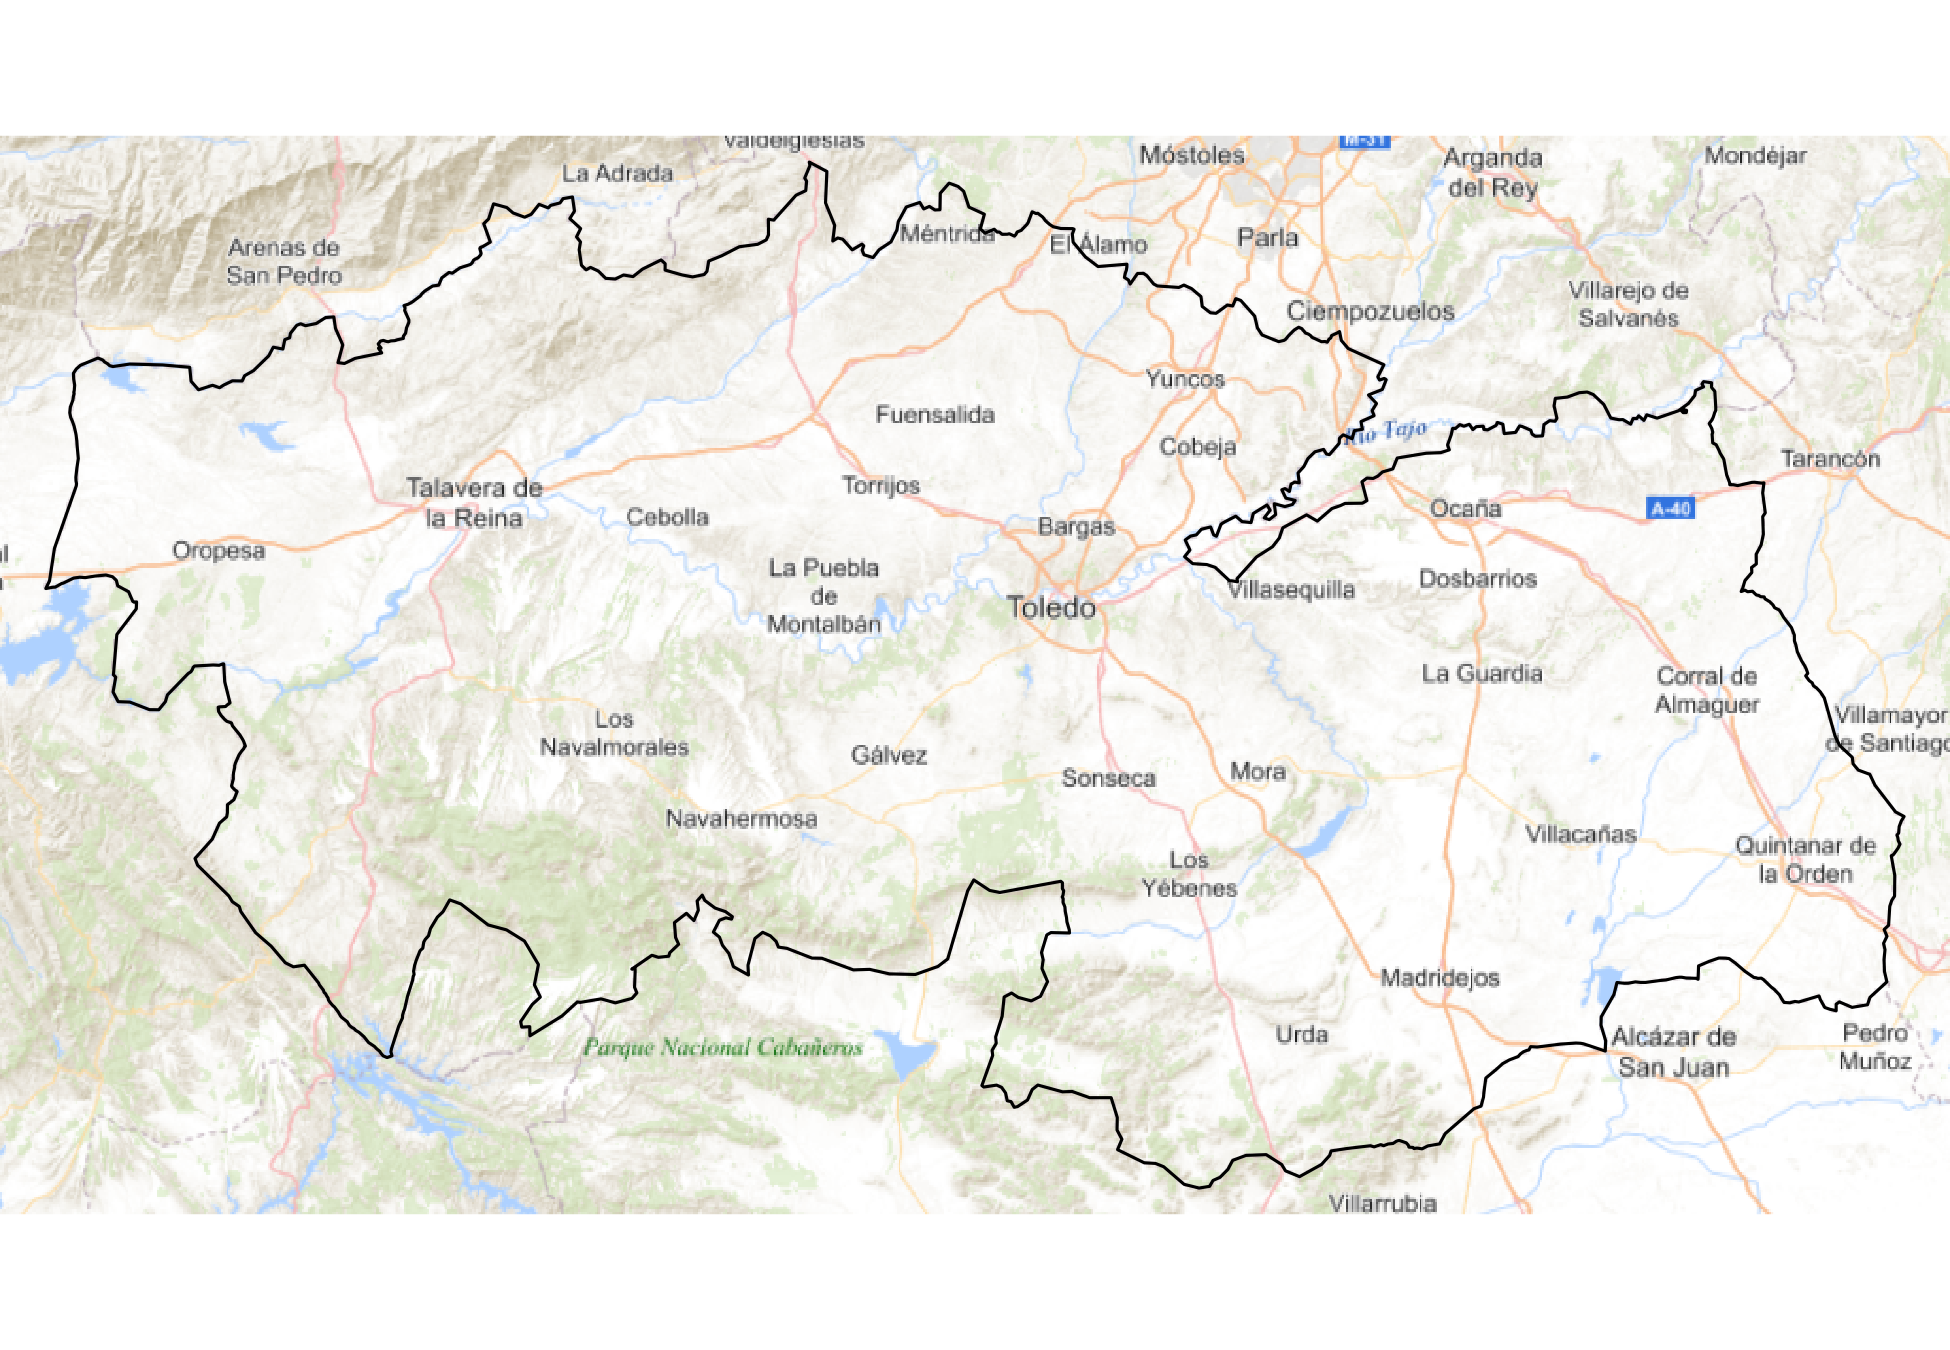
\includegraphics[width=0.6\linewidth]{_main_files/figure-latex/raster-multilayer-1} 

}

\caption{Datos ráster con varias bandas}\label{fig:raster-multilayer}
\end{figure}

El ráster se puede descomponer en las tres capas RGB mencionadas anteriormente:

\begin{table}

\caption{\label{tab:detalle-pixel-multicapa}Datos de un ráster multicapa (detalle)}
\centering
\begin{tabular}[t]{r|r|r|r|r}
\hline
x & y & lyr.1 & lyr.2 & lyr.3\\
\hline
-5.466412 & 40.34418 & 215.2128 & 208.1061 & 190.5410\\
\hline
-5.463875 & 40.34418 & 228.0369 & 223.1854 & 211.2115\\
\hline
-5.461338 & 40.34418 & 229.3495 & 224.3414 & 213.4325\\
\hline
-5.458800 & 40.34418 & 215.8592 & 208.8660 & 191.2922\\
\hline
-5.456263 & 40.34418 & 219.2696 & 212.8231 & 196.6812\\
\hline
-5.453725 & 40.34418 & 235.0954 & 231.4222 & 222.4115\\
\hline
-5.451188 & 40.34418 & 240.3514 & 237.9094 & 231.4736\\
\hline
-5.448651 & 40.34418 & 237.2358 & 233.7561 & 226.2005\\
\hline
-5.446113 & 40.34418 & 229.9570 & 225.3262 & 214.6201\\
\hline
-5.443576 & 40.34418 & 226.7812 & 221.6796 & 209.2929\\
\hline
-5.441038 & 40.34418 & 222.3593 & 216.5022 & 202.0188\\
\hline
-5.438501 & 40.34418 & 220.9312 & 214.9060 & 200.0306\\
\hline
-5.435964 & 40.34418 & 224.7755 & 219.2661 & 206.2156\\
\hline
-5.433426 & 40.34418 & 222.0479 & 216.0124 & 201.6103\\
\hline
-5.430889 & 40.34418 & 225.0516 & 219.8074 & 207.0263\\
\hline
\end{tabular}
\end{table}

\begin{figure}

{\centering 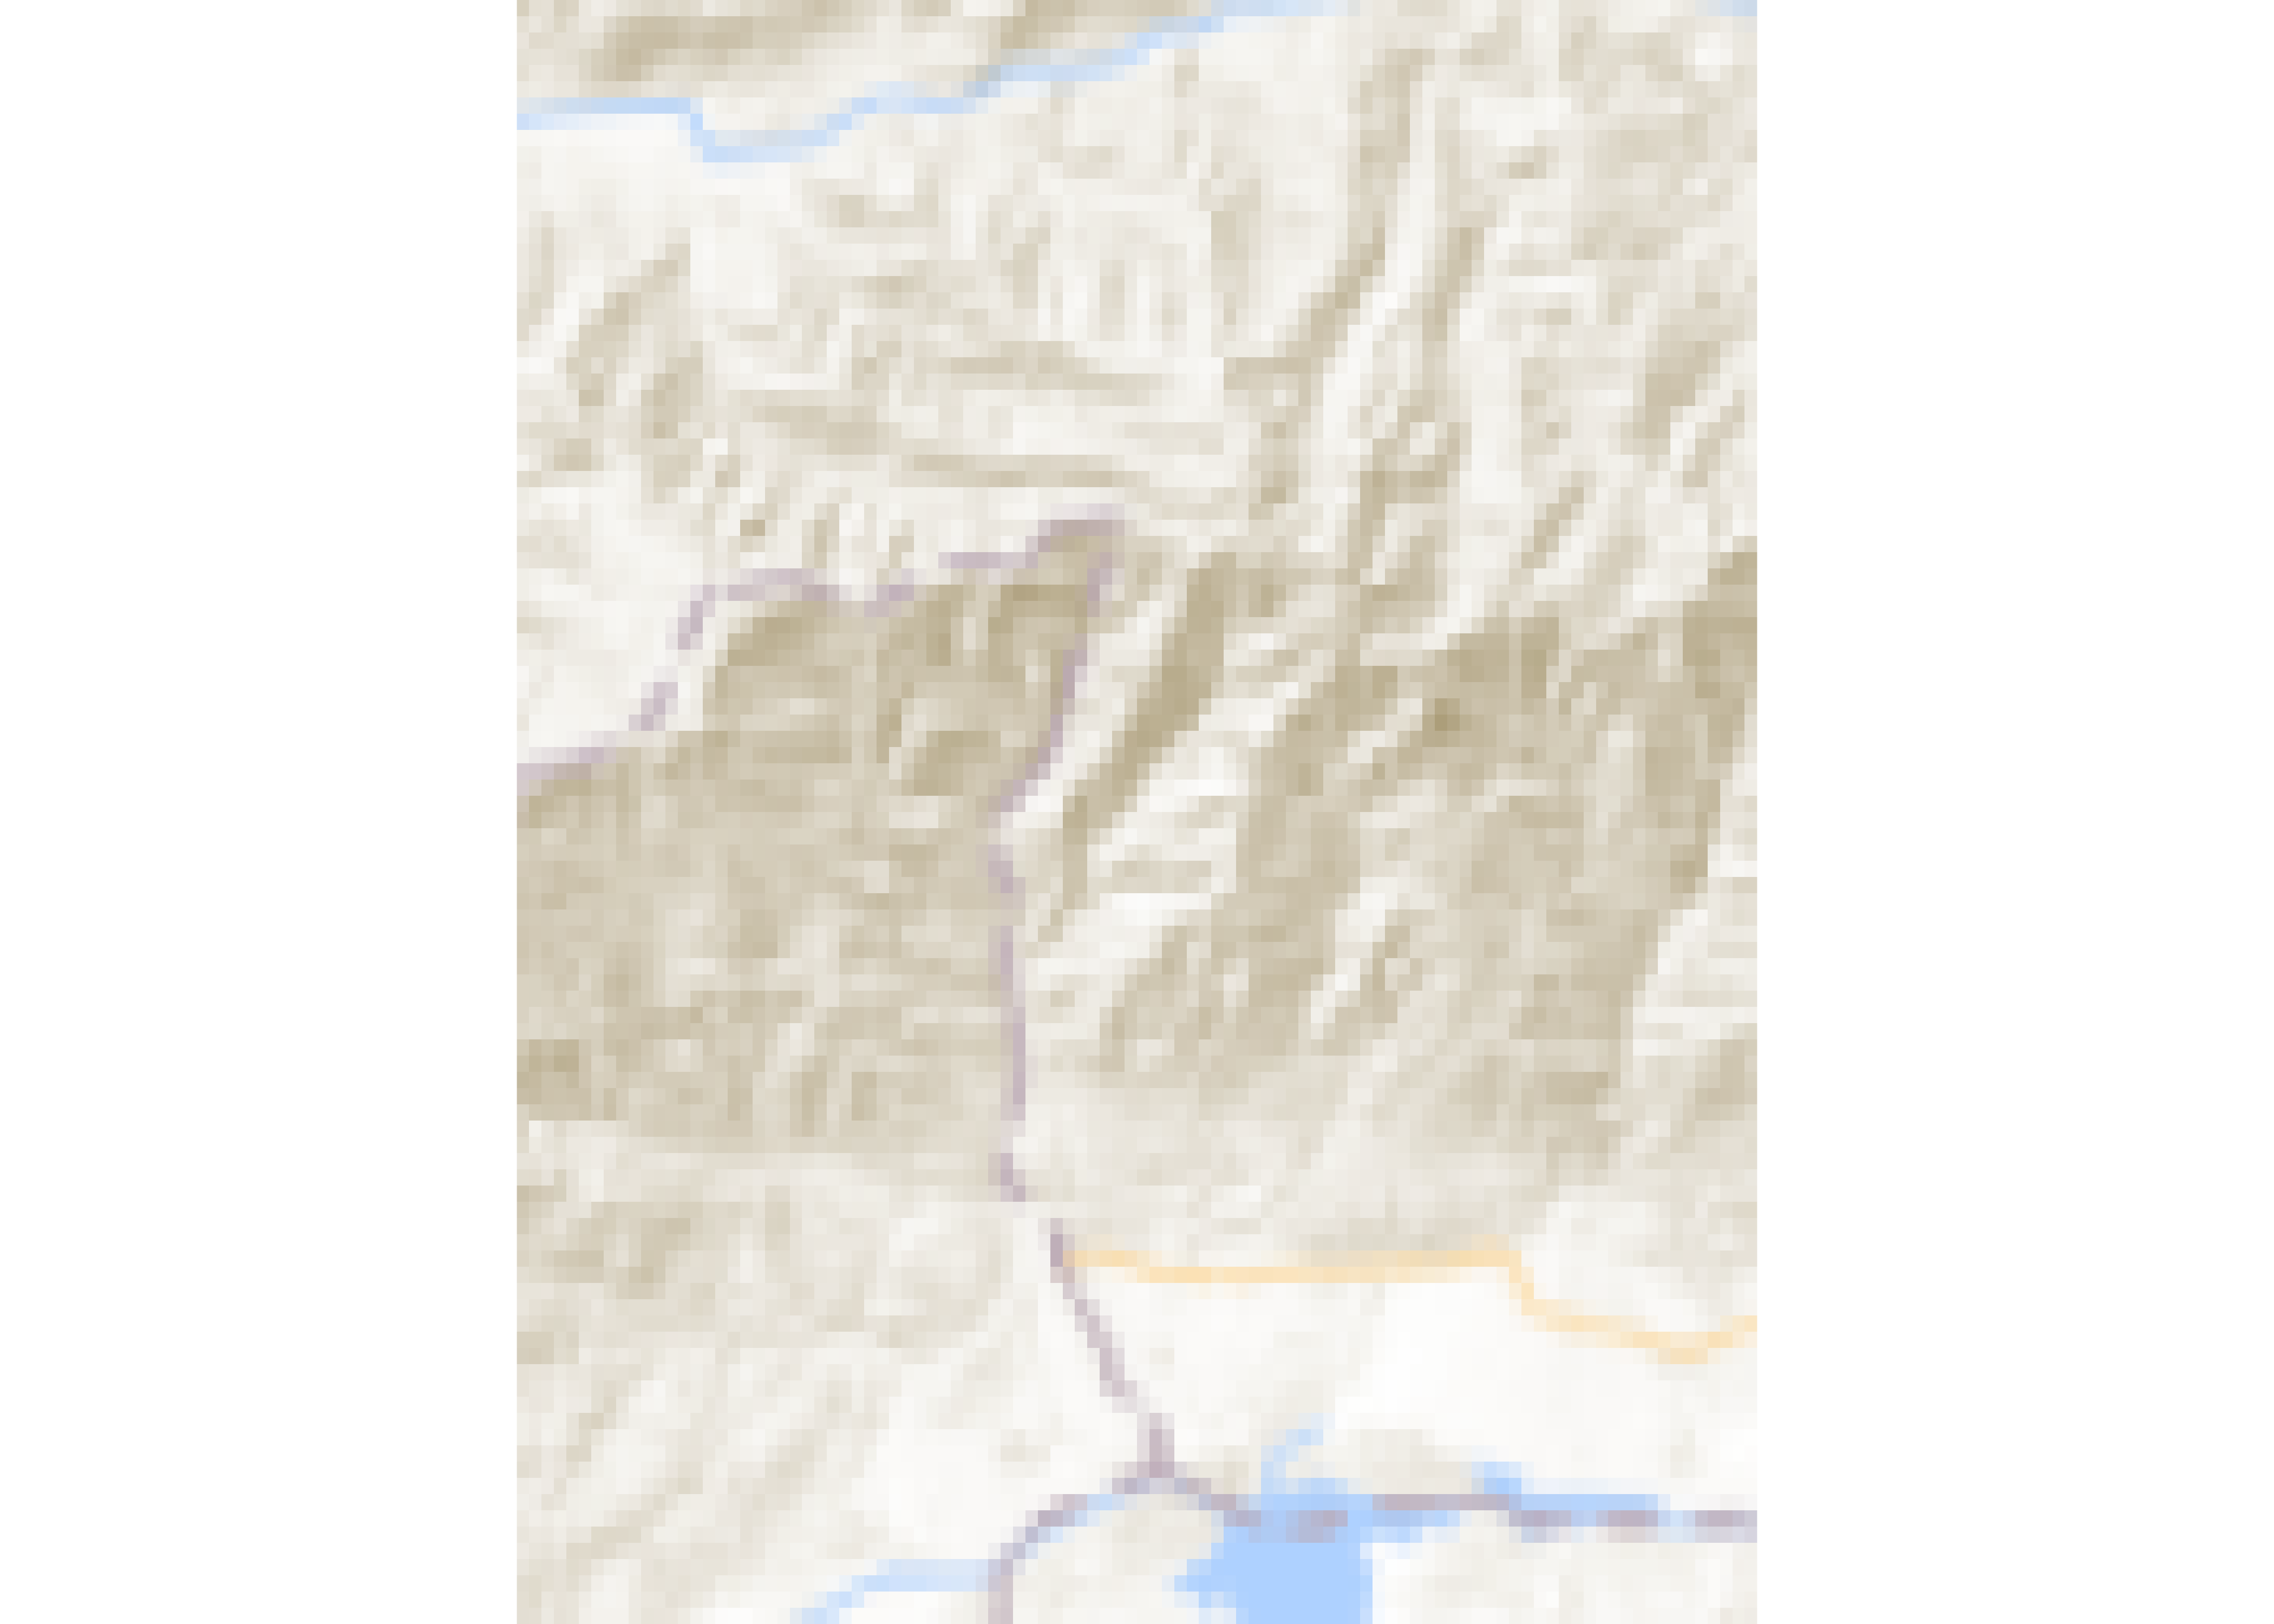
\includegraphics[width=0.6\linewidth]{_main_files/figure-latex/detalle-pixel-multicapa-1} 

}

\caption{Datos ráster multicapa: Descomposición}\label{fig:detalle-pixel-multicapa-1}
\end{figure}
\begin{figure}

{\centering 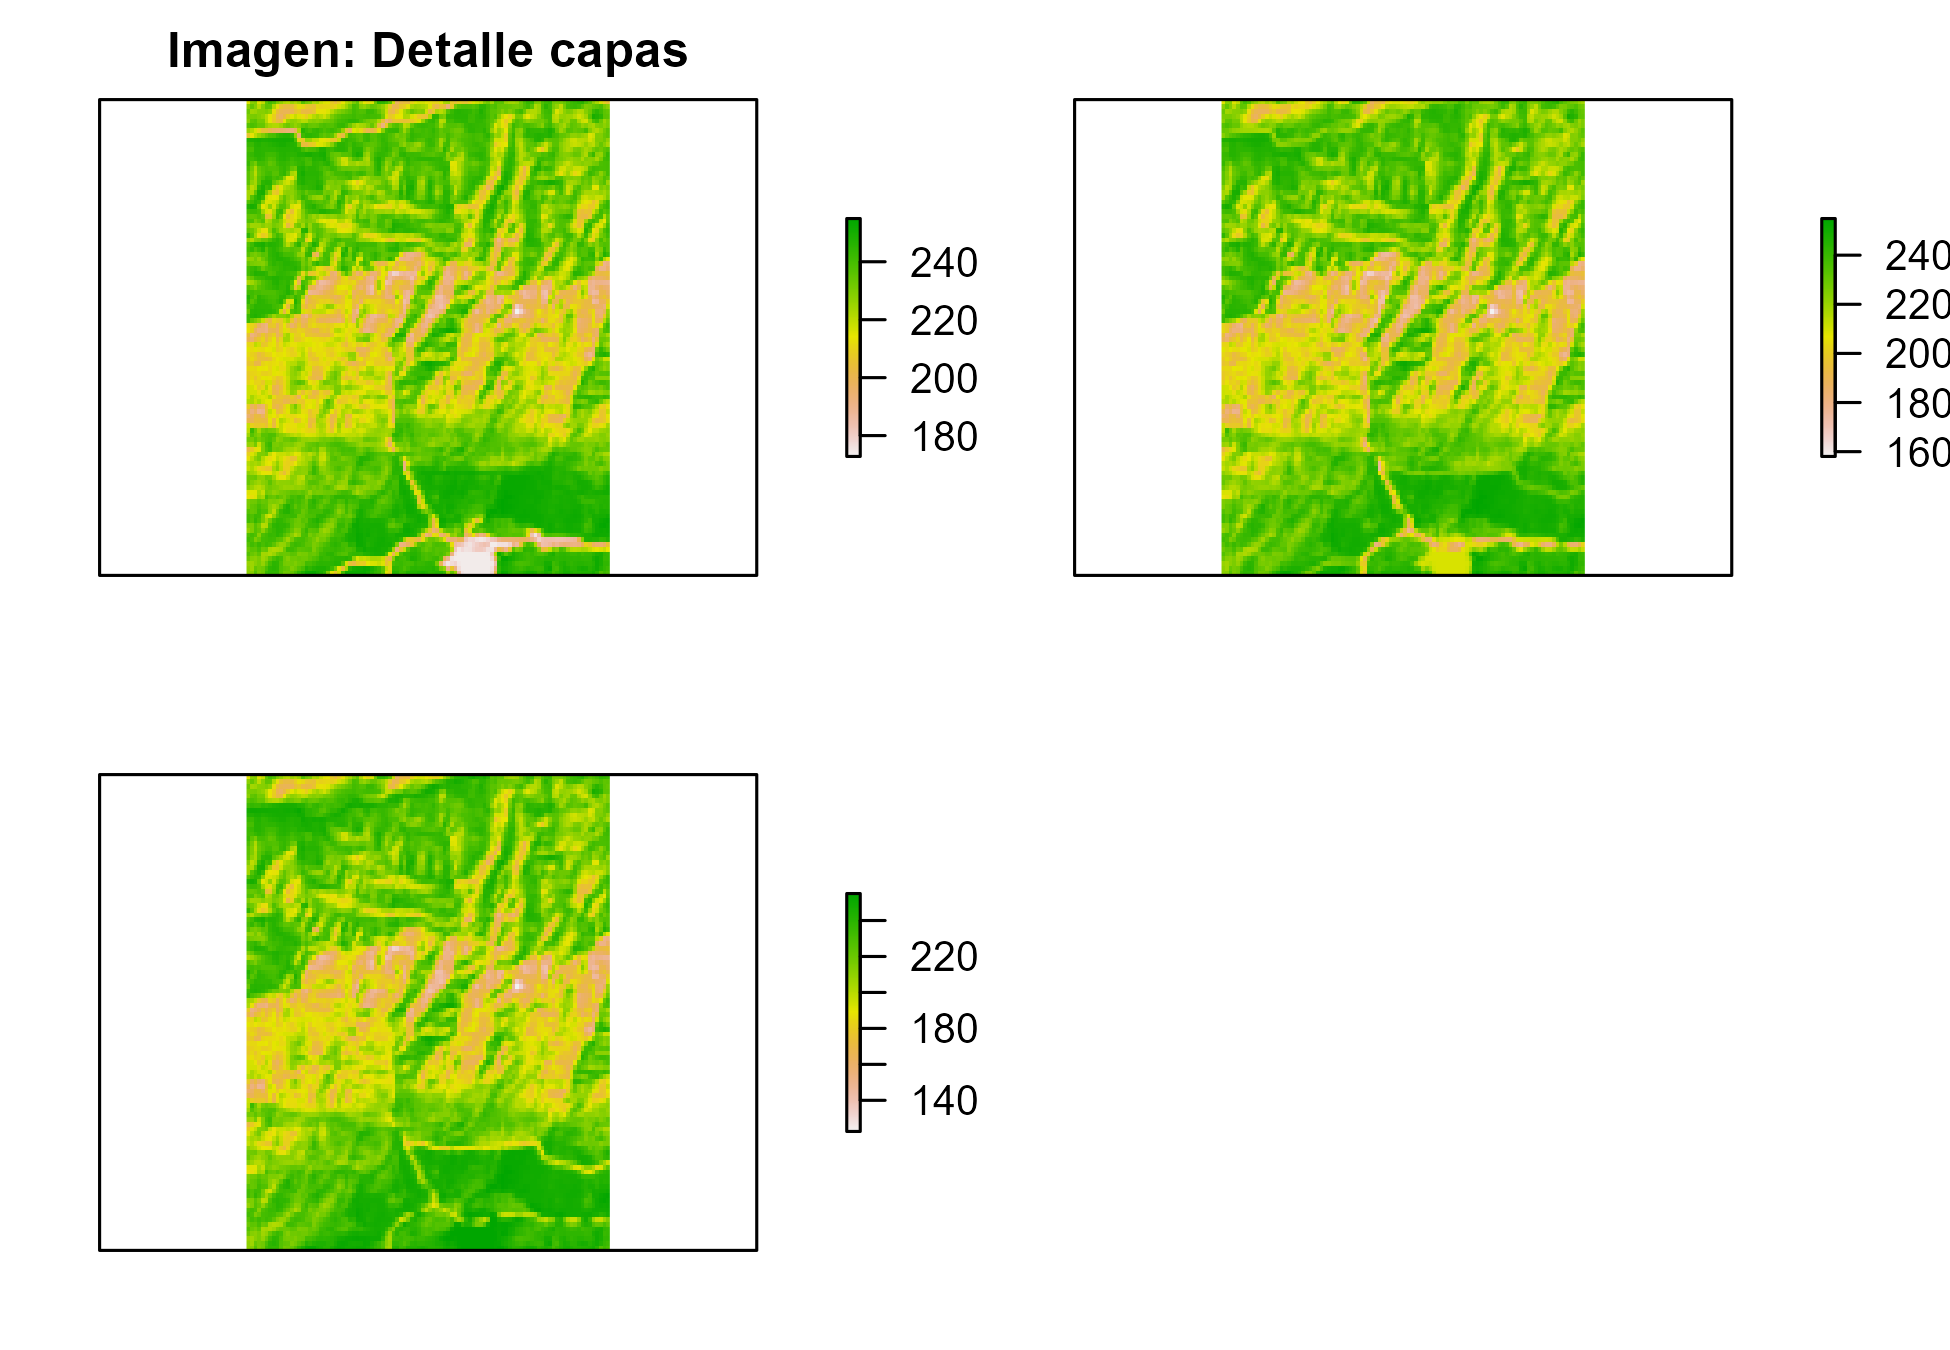
\includegraphics[width=0.6\linewidth]{_main_files/figure-latex/detalle-pixel-multicapa-2} 

}

\caption{Datos ráster multicapa: Descomposición}\label{fig:detalle-pixel-multicapa-2}
\end{figure}

\hypertarget{CRS}{%
\section{Sistema de Referencia de Coordenadas (CRS)}\label{CRS}}

Un sistema de referencia de coordenadas (o CRS por sus siglas en inglés,
\textbf{Coordinate Reference System}) permite relacionar datos espaciales con su
localización en la superficie terrestre.

\textbf{Los CRS constituyen por tanto un aspecto fundamental en el análisis y
representación de datos espaciales}, ya que nos permiten identificar con
exactitud la posición de los datos sobre el globo terráqueo.

Así mismo, cuando se trabaja con datos espaciales provenientes de distintas
fuentes de información, es necesario comprobar que dichos datos se encuentran
definidos en el mismo CRS:

\begin{figure}

{\centering 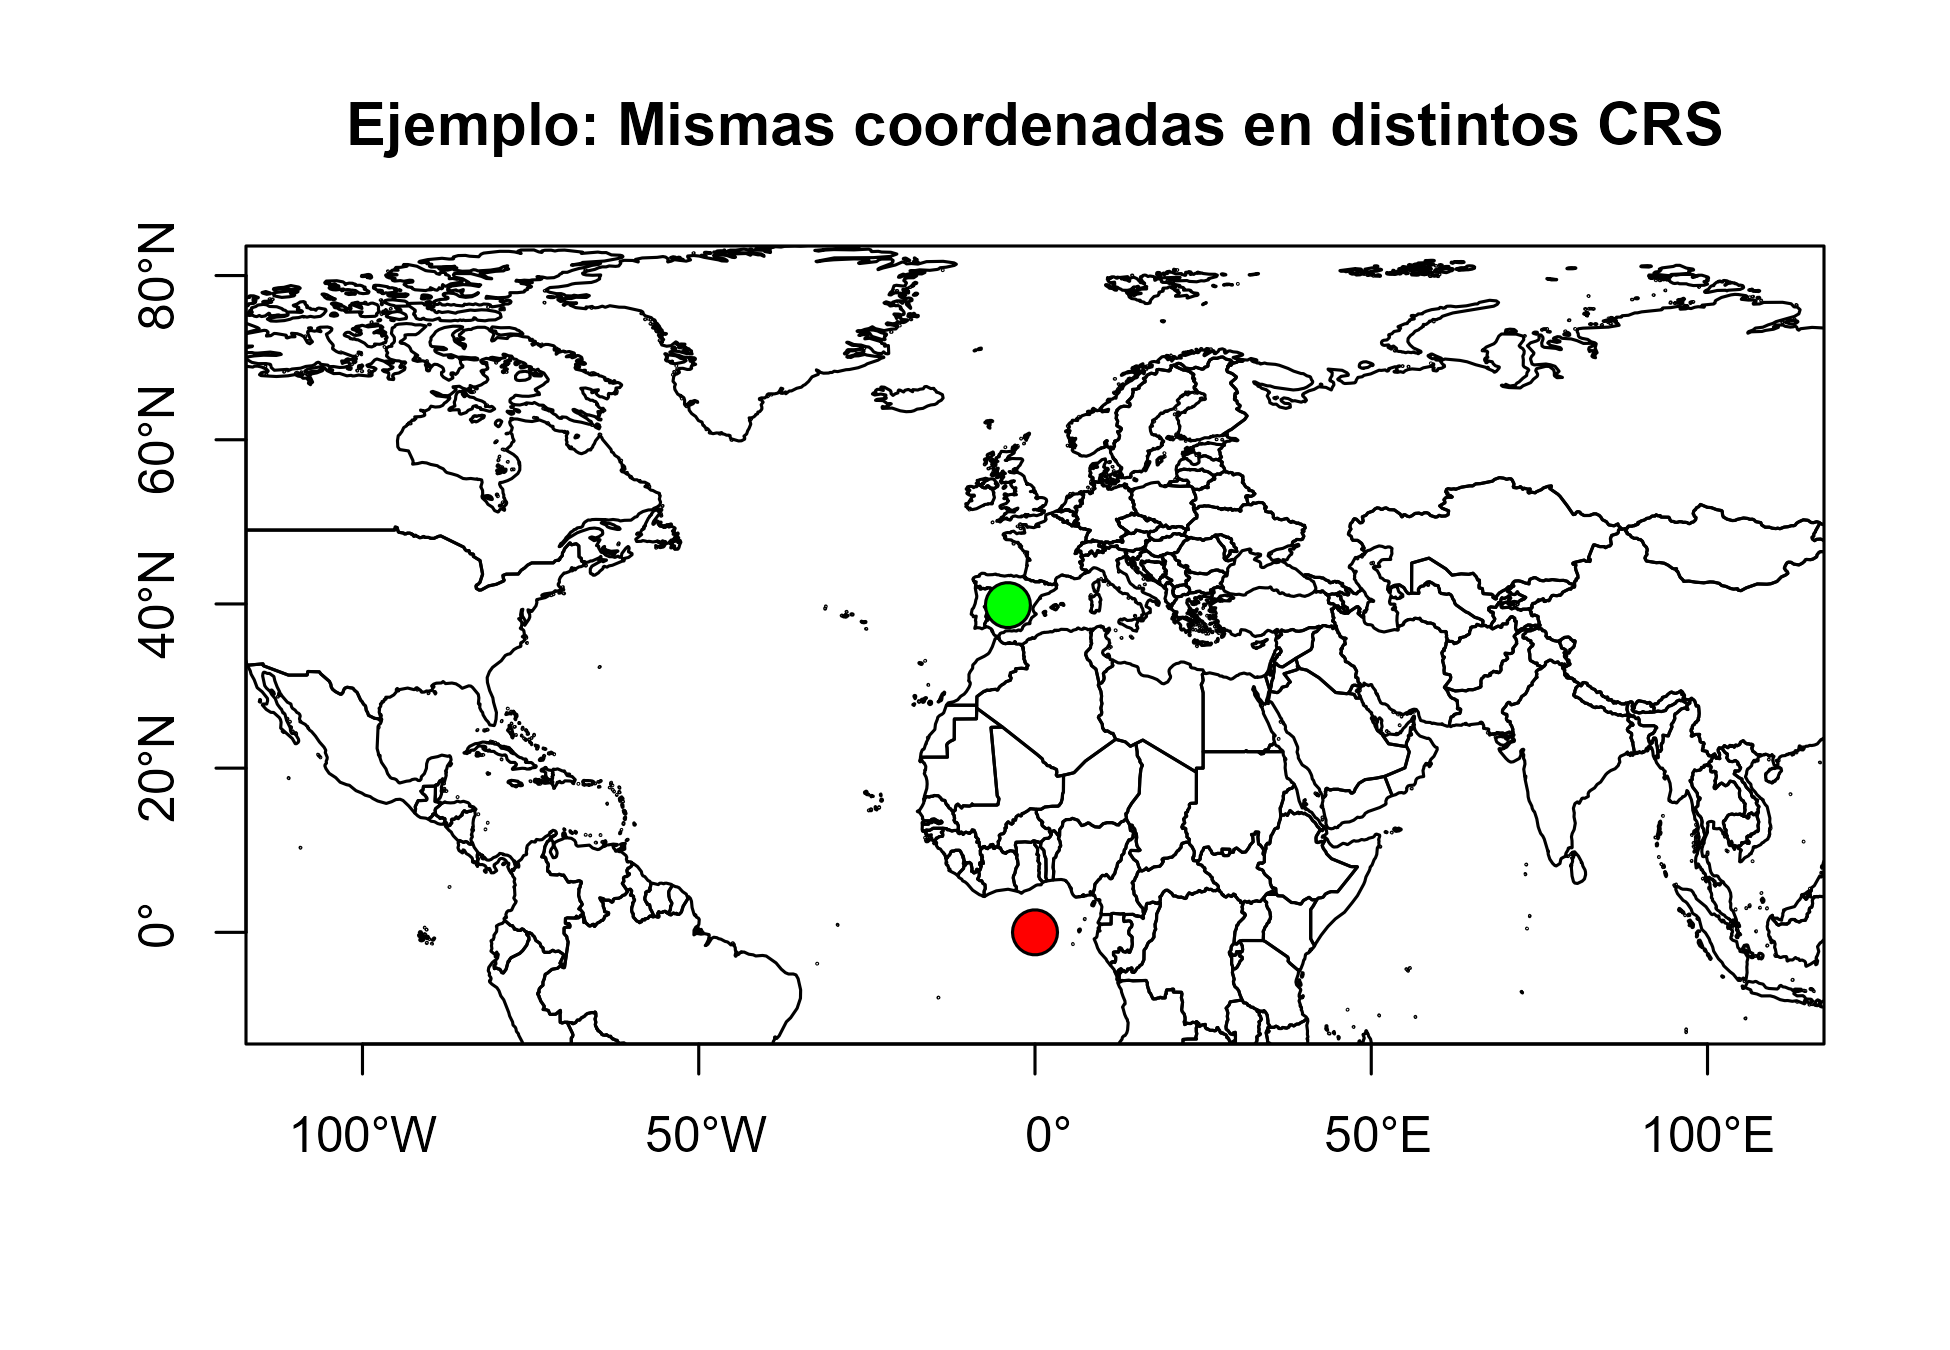
\includegraphics[width=0.6\linewidth]{_main_files/figure-latex/datosdesalineados-1} 

}

\caption{Representación de mismos valores de coordenadas en distintos CRS}\label{fig:datosdesalineados}
\end{figure}

En la Fig. \ref{fig:datosdesalineados}, ambos puntos (verde y rojo) tienen los
mismos valores de coordenadas en los ejes X e Y, en este caso las
correspondientes a la ciudad de Toledo. Sin embargo, presentan distintos CRS.
Por este motivo, al representar ambos puntos en un mapa, se observa que no se
están refiriendo a la misma localización geográfica. Esto es así porque el CRS
define la referencia (punto x=0 e y =0) y las unidades de los ejes (grados,
metros, millas).

Como conclusión, \textbf{además de disponer de las coordenadas de los datos
espaciales, es necesario conocer el CRS en el que están definidos para conocer
de manera exacta su localización geográfica.} Además, nótese que para cualquier
\textbf{análisis de datos espaciales} es necesario que todos los geodatos \textbf{se
encuentren referenciados en el mismo CRS}. Esto se consigue transformando (o
proyectando) los datos a un CRS común, nunca sobreescribiendo el CRS de los
mismos.

\hypertarget{tipos-de-crs}{%
\subsection{Tipos de CRS}\label{tipos-de-crs}}

A continuación se definen los dos grandes tipos de CRS, los CRS geográficos y
los CRS proyectados.

\hypertarget{crs-geogruxe1ficos}{%
\subsubsection{CRS geográficos}\label{crs-geogruxe1ficos}}

Los CRS geográficos son aquellos en los que los parámetros empleados para
localizar una posición espacial son la latitud y la longitud:

\begin{itemize}
\item
  \textbf{Latitud}: Es la distancia angular expresada en grados sobre el plano
  definido por el ecuador terrestre. Determina la posición sobre de una
  localización en el eje Norte-Sur de la Tierra y toma valores en el rango
  \([-90º,90º]\) . Las líneas imaginarias determinadas por una sucesión de
  puntos con la misma latitud a lo largo del eje Este-Oeste se denominan
  \textbf{paralelos} (Ver Fig. \ref{fig:meridianos}).
\item
  \textbf{Longitud}: Es la distancia angular expresada en grados sobre el plano
  definido por el meridiano de Greenwich. Determina la posición sobre de una
  localización en el eje Este-Oeste de la Tierra y toma valores en el rango
  \([-180º,180º]\) . Las líneas imaginarias determinadas por una sucesión de
  puntos con la misma longitud a lo largo del eje Este-Oeste se denominan
  \textbf{meridianos} (Ver Fig. \ref{fig:meridianos}).
\end{itemize}

\begin{figure}

{\centering 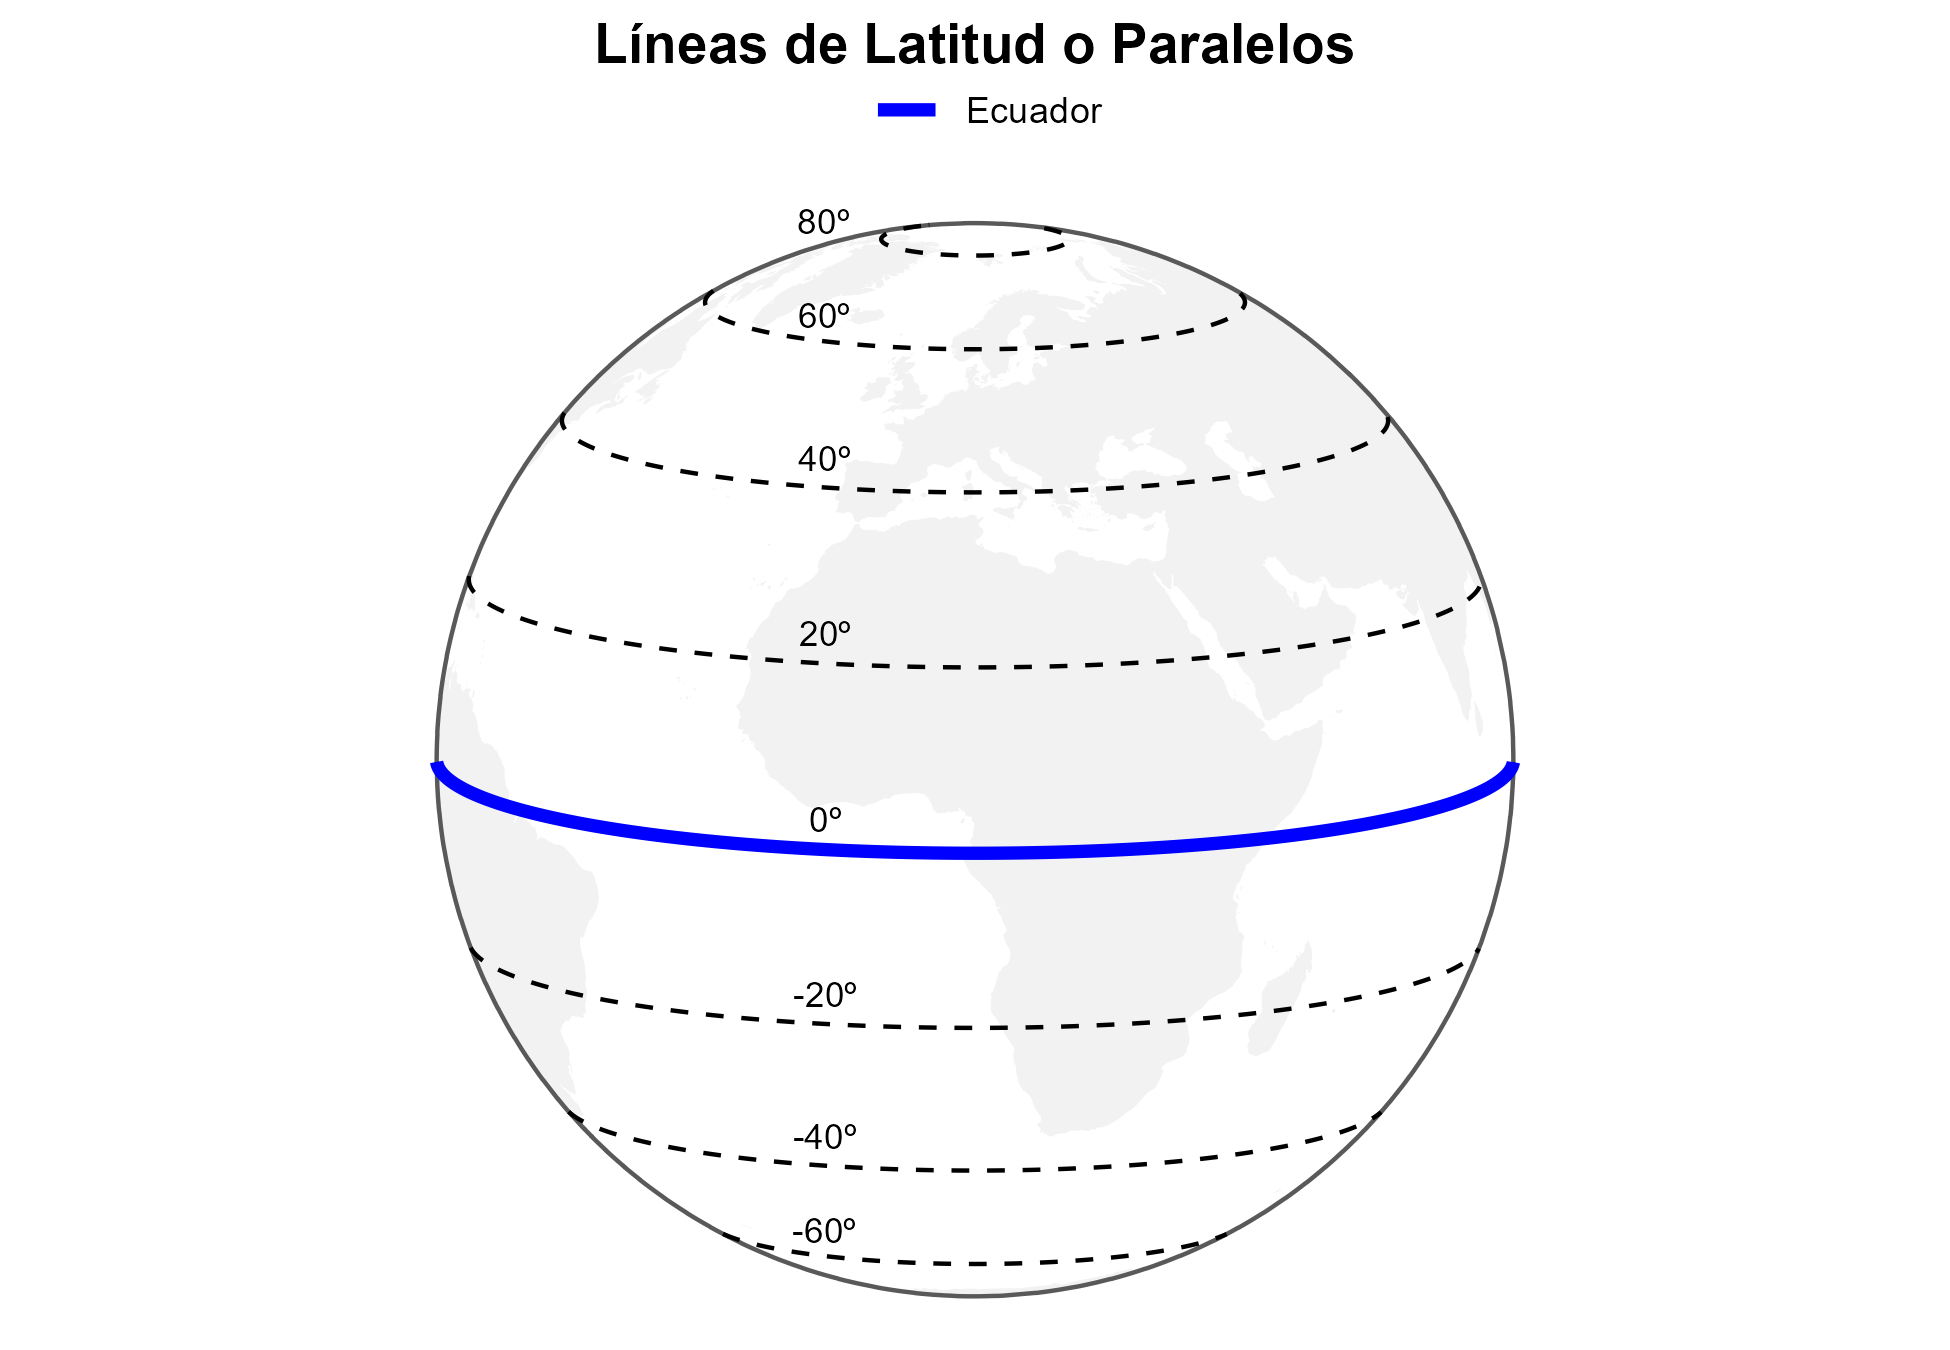
\includegraphics[width=0.5\linewidth]{_main_files/figure-latex/meridianos-1} 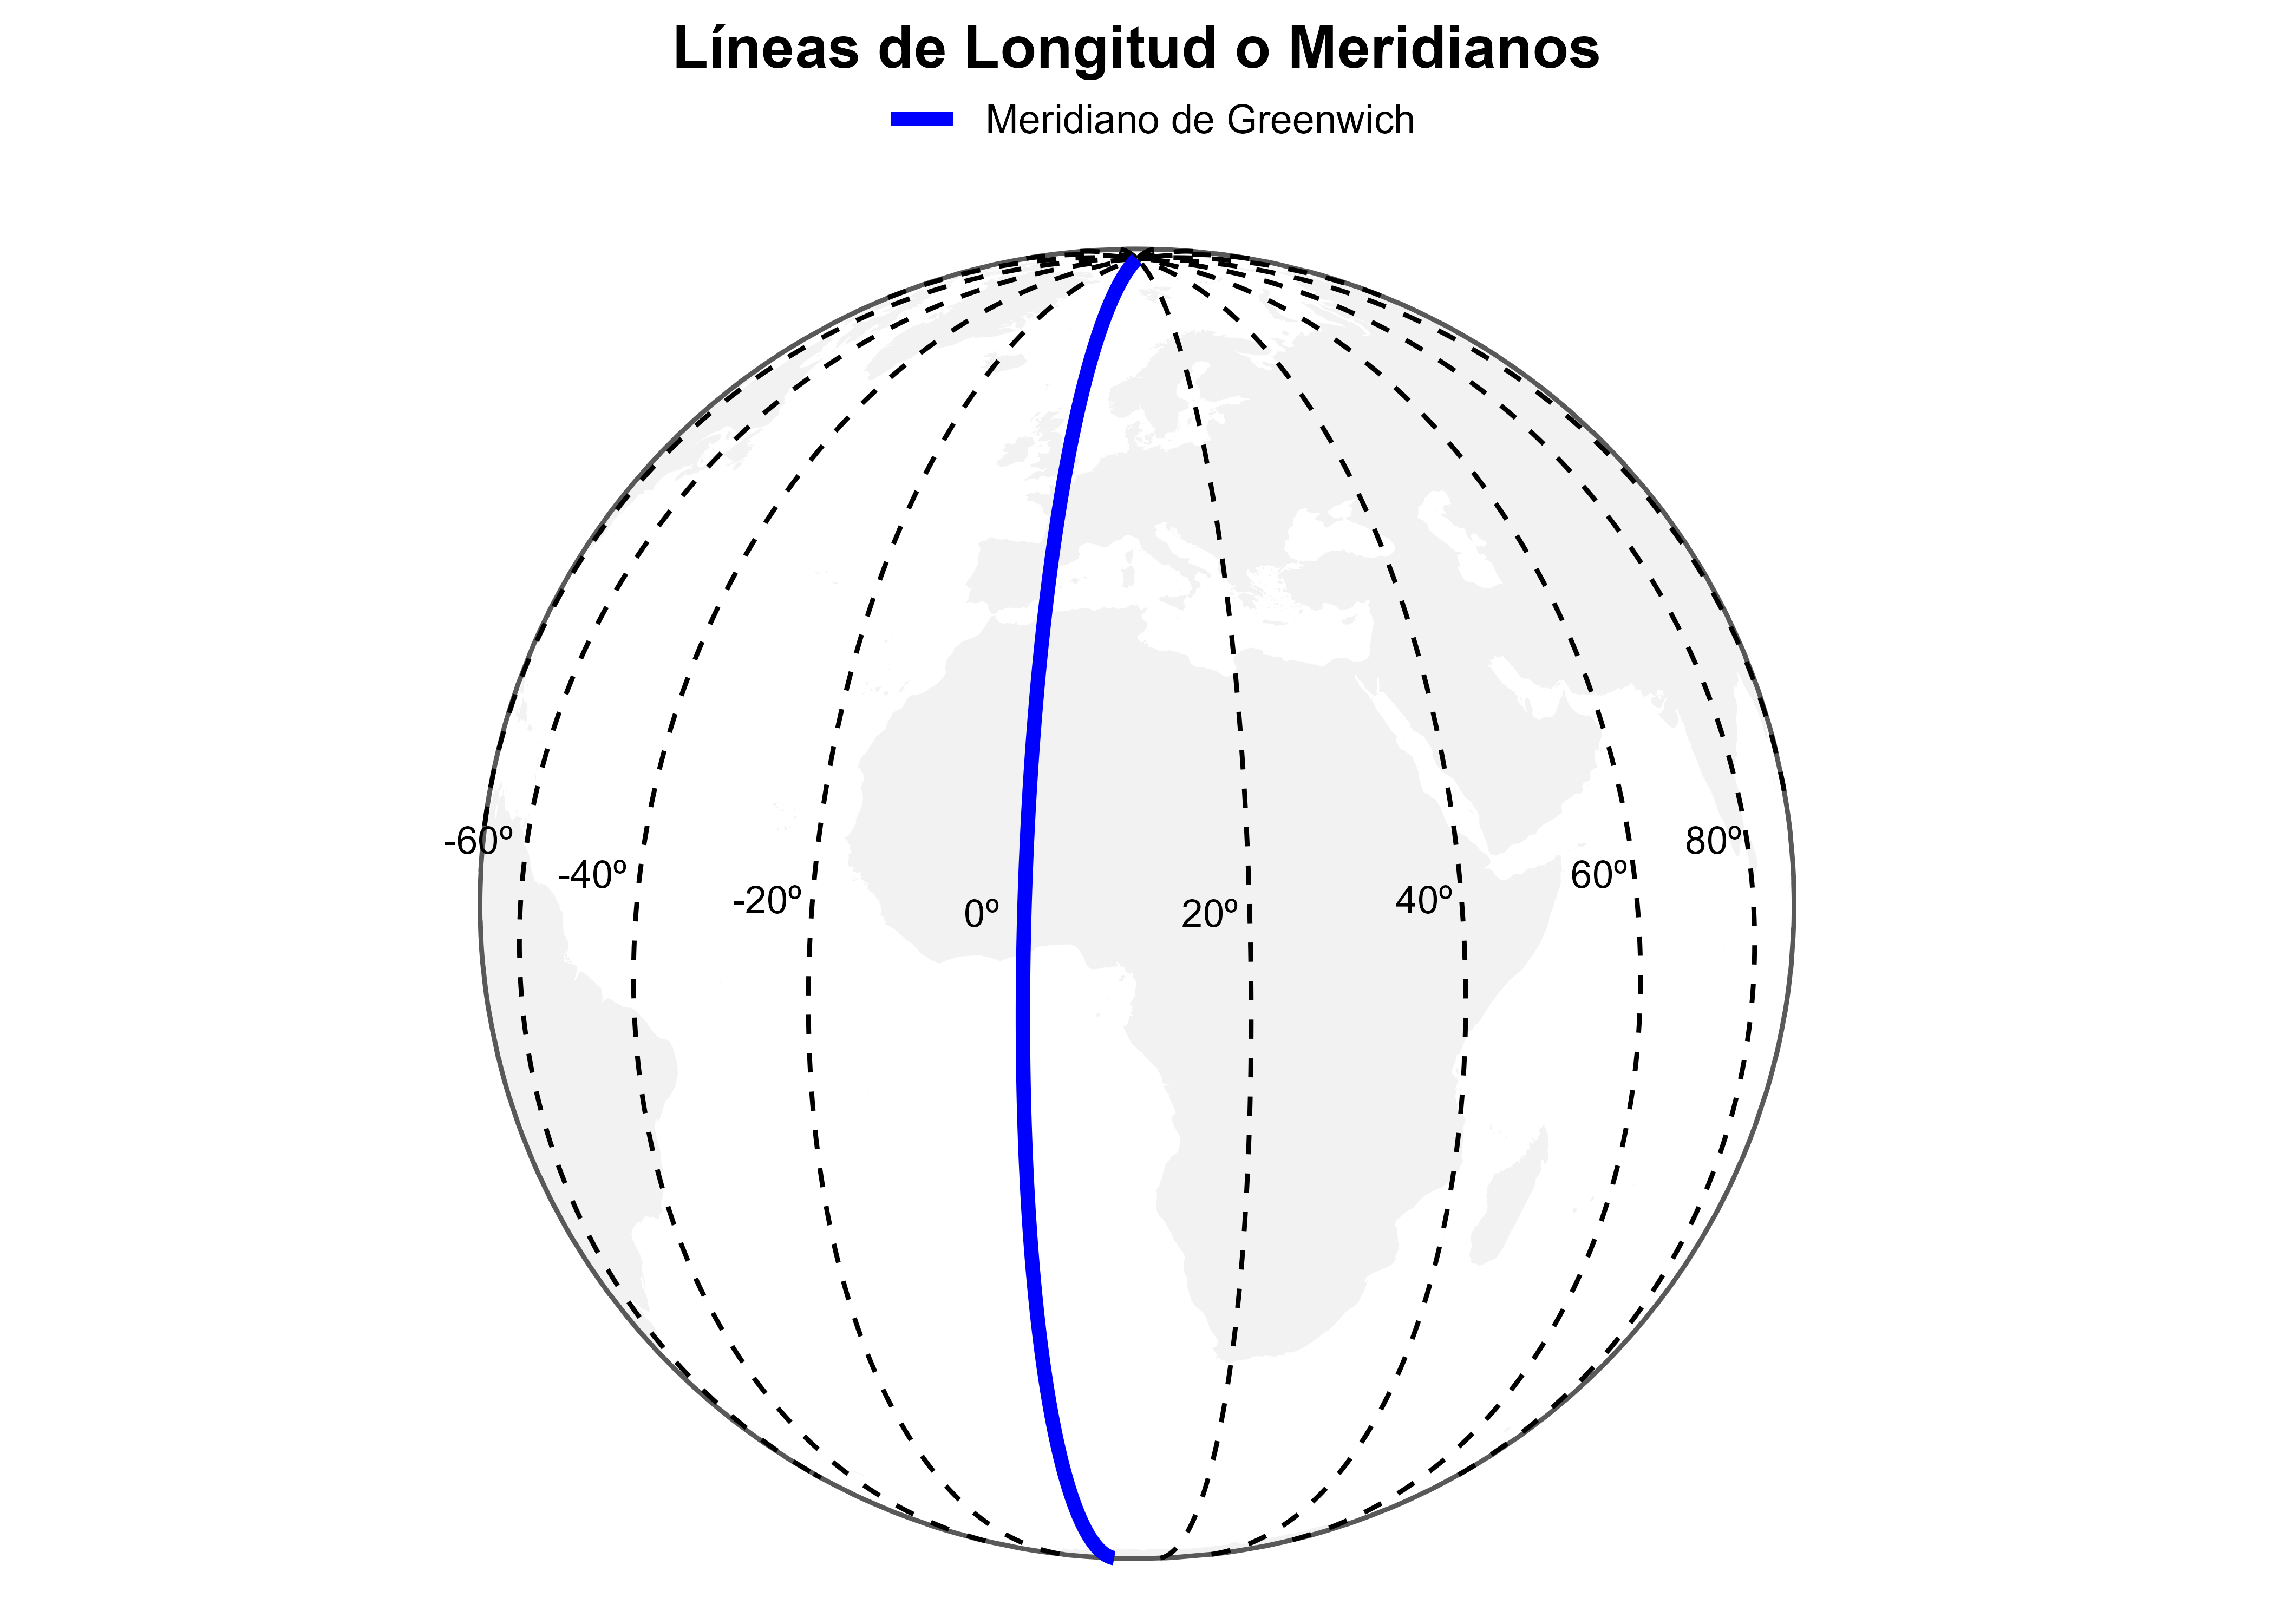
\includegraphics[width=0.5\linewidth]{_main_files/figure-latex/meridianos-2} 

}

\caption{Paralelos y Meridianos terrestres}\label{fig:meridianos}
\end{figure}

Es muy importante destacar que en un sistema de coordenadas geográfico, es
decir, basado en latitudes y longitudes, las \textbf{distancias} entre dos puntos
representan \textbf{distancias angulares}. Por ejemplo, la distancia entre el
meridiano de Greenwich y el meridiano correspondiente a la longitud 20º siempre
es de +20º. Sin embargo, debido a la forma esférica de la Tierra, la longitud en
metros entre ambos meridianos no es constante.

\begin{figure}

{\centering 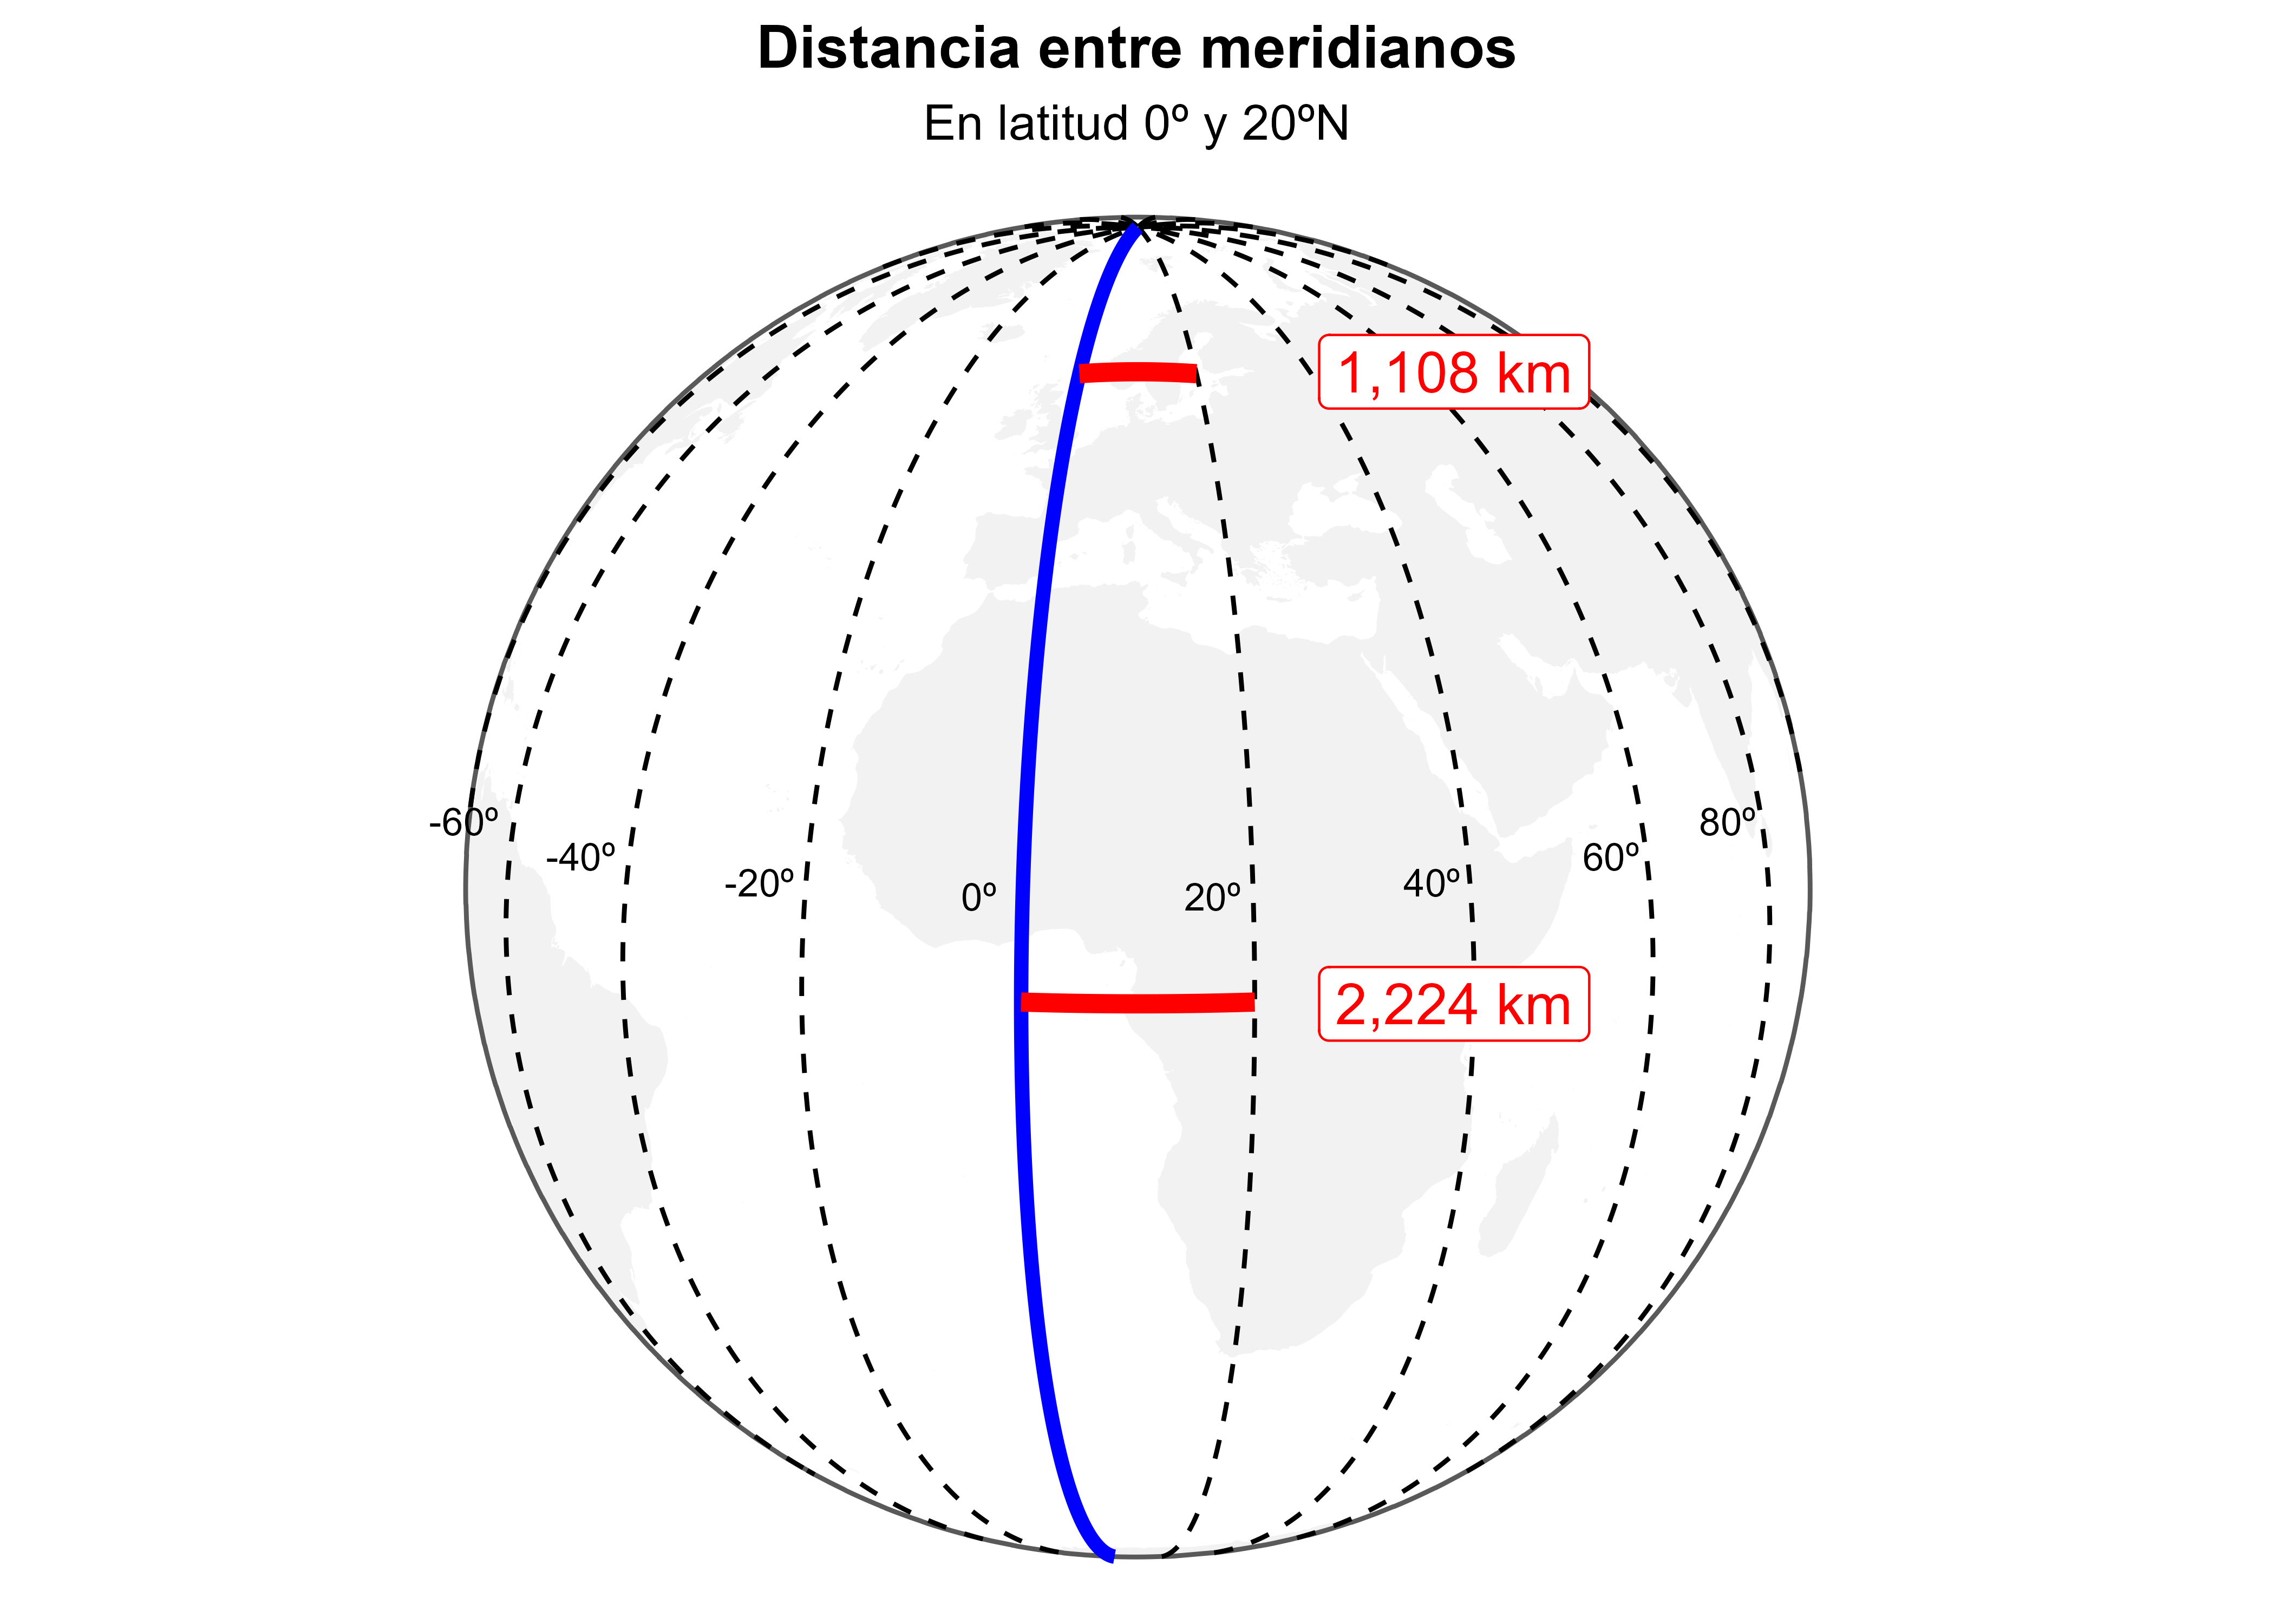
\includegraphics[width=0.6\linewidth]{_main_files/figure-latex/distang-1} 

}

\caption{Distancia entre meridianos en distintas latitudes}\label{fig:distang}
\end{figure}

\hypertarget{crs-proyectados}{%
\subsubsection{CRS proyectados}\label{crs-proyectados}}

La representación de formas tridimensionales en un soporte plano (dos
dimensiones) presenta algunos retos. Por ello, es habitual trabajar con
proyecciones de mapas.

Una \textbf{proyección geográfica} es un método para reducir la superficie de la
esfera terrestre a un sistema cartesiano de dos dimensiones. Para ello, es
necesario transformar las coordenadas longitud y latitud en coordenadas
cartesianas x e y.

Es importante destacar que las proyecciones pueden incluir un punto de origen
(X=0, Y=0) y unas unidades de distancia (habitualmente metros) específicas. Por
ejemplo, la \textbf{proyección cónica equiáreas de Albers} (específica para Estados
Unidos) define su punto de referencia (0,0) en la latitud 40º N y longitud 96º,
y la unidad de variación están definida en metros. De ahí la importancia de
conocer el CRS de los datos geográficos, como se expuso al principio de este
tema.

El Anexo \ref{crsproy} proporciona más información sobre los tipos de CRS
proyectados.

\hypertarget{trabajando-con-proyecciones-en-r}{%
\subsection{Trabajando con proyecciones en R}\label{trabajando-con-proyecciones-en-r}}

Existe toda una serie de proyecciones predefinidas, identificadas mediante los
\textbf{códigos EPSG, ESRI, WKT} o proj4 (en desuso en R, pero todavía admitidos).
Existen varios recursos web donde se pueden consultar y seleccionar los códigos
correspondientes:

\begin{itemize}
\item
  \url{https://epsg.io/}
\item
  \url{https://spatialreference.org/}
\item
  \url{https://proj.org/operations/projections/index.html}
\end{itemize}

Algunos de los códigos de proyecciones que es fundamental conocer son:

\begin{itemize}
\item
  \textbf{EPSG: 4326}: Proyección correspondiente a WGS 84, que es el sistema usado
  por los sistemas GPS. Cuando trabajemos con coordenadas geográficas
  longitud/latitud, este es habitualmente el CRS de referencia.
\item
  \textbf{EPSG: 3857}: Código correspondiente a la proyección de Mercator, usada
  habitualmente por servicios como Google Maps, etc.
\end{itemize}

Se pueden consultar otros CRS de uso común en España en la página del
\href{https://www.mapa.gob.es/es/cartografia-y-sig/ide/directorio_datos_servicios/caracteristicas_wms.aspx}{Ministerio de Agricultura, Pesca y
Alimentación}

En la sección \ref{quecrsuso} veremos cómo encontrar un CRS usando el paquete
\texttt{crsuggest}.

El paquete \texttt{sf} permite obtener los parámetros de cualquier proyección mediante
la función \texttt{st\_crs()}:

\textbf{(i) EPSG WGS 84 (Sistema Global GPS): EPSG 4326}

\begin{Shaded}
\begin{Highlighting}[]
\FunctionTok{library}\NormalTok{(sf)}

\CommentTok{\# Ejemplo: EPSG WGS 84 (Sistema Global GPS): EPSG 4326}
\FunctionTok{st\_crs}\NormalTok{(}\DecValTok{4326}\NormalTok{)}
\CommentTok{\#\textgreater{} Coordinate Reference System:}
\CommentTok{\#\textgreater{}   User input: EPSG:4326 }
\CommentTok{\#\textgreater{}   wkt:}
\CommentTok{\#\textgreater{} GEOGCRS["WGS 84",}
\CommentTok{\#\textgreater{}     DATUM["World Geodetic System 1984",}
\CommentTok{\#\textgreater{}         ELLIPSOID["WGS 84",6378137,298.257223563,}
\CommentTok{\#\textgreater{}             LENGTHUNIT["metre",1]]],}
\CommentTok{\#\textgreater{}     PRIMEM["Greenwich",0,}
\CommentTok{\#\textgreater{}         ANGLEUNIT["degree",0.0174532925199433]],}
\CommentTok{\#\textgreater{}     CS[ellipsoidal,2],}
\CommentTok{\#\textgreater{}         AXIS["geodetic latitude (Lat)",north,}
\CommentTok{\#\textgreater{}             ORDER[1],}
\CommentTok{\#\textgreater{}             ANGLEUNIT["degree",0.0174532925199433]],}
\CommentTok{\#\textgreater{}         AXIS["geodetic longitude (Lon)",east,}
\CommentTok{\#\textgreater{}             ORDER[2],}
\CommentTok{\#\textgreater{}             ANGLEUNIT["degree",0.0174532925199433]],}
\CommentTok{\#\textgreater{}     USAGE[}
\CommentTok{\#\textgreater{}         SCOPE["Horizontal component of 3D system."],}
\CommentTok{\#\textgreater{}         AREA["World."],}
\CommentTok{\#\textgreater{}         BBOX[{-}90,{-}180,90,180]],}
\CommentTok{\#\textgreater{}     ID["EPSG",4326]]}
\end{Highlighting}
\end{Shaded}

\textbf{(ii) ESRI North America Albers Equal Area Conic: ESRI:102008}

\begin{Shaded}
\begin{Highlighting}[]
\CommentTok{\# Usando código ESRI North America Albers Equal Area Conic}

\FunctionTok{st\_crs}\NormalTok{(}\StringTok{"ESRI:102008"}\NormalTok{)}
\CommentTok{\#\textgreater{} Coordinate Reference System:}
\CommentTok{\#\textgreater{}   User input: ESRI:102008 }
\CommentTok{\#\textgreater{}   wkt:}
\CommentTok{\#\textgreater{} PROJCRS["North\_America\_Albers\_Equal\_Area\_Conic",}
\CommentTok{\#\textgreater{}     BASEGEOGCRS["NAD83",}
\CommentTok{\#\textgreater{}         DATUM["North American Datum 1983",}
\CommentTok{\#\textgreater{}             ELLIPSOID["GRS 1980",6378137,298.257222101,}
\CommentTok{\#\textgreater{}                 LENGTHUNIT["metre",1]]],}
\CommentTok{\#\textgreater{}         PRIMEM["Greenwich",0,}
\CommentTok{\#\textgreater{}             ANGLEUNIT["Degree",0.0174532925199433]]],}
\CommentTok{\#\textgreater{}     CONVERSION["North\_America\_Albers\_Equal\_Area\_Conic",}
\CommentTok{\#\textgreater{}         METHOD["Albers Equal Area",}
\CommentTok{\#\textgreater{}             ID["EPSG",9822]],}
\CommentTok{\#\textgreater{}         PARAMETER["Latitude of false origin",40,}
\CommentTok{\#\textgreater{}             ANGLEUNIT["Degree",0.0174532925199433],}
\CommentTok{\#\textgreater{}             ID["EPSG",8821]],}
\CommentTok{\#\textgreater{}         PARAMETER["Longitude of false origin",{-}96,}
\CommentTok{\#\textgreater{}             ANGLEUNIT["Degree",0.0174532925199433],}
\CommentTok{\#\textgreater{}             ID["EPSG",8822]],}
\CommentTok{\#\textgreater{}         PARAMETER["Latitude of 1st standard parallel",20,}
\CommentTok{\#\textgreater{}             ANGLEUNIT["Degree",0.0174532925199433],}
\CommentTok{\#\textgreater{}             ID["EPSG",8823]],}
\CommentTok{\#\textgreater{}         PARAMETER["Latitude of 2nd standard parallel",60,}
\CommentTok{\#\textgreater{}             ANGLEUNIT["Degree",0.0174532925199433],}
\CommentTok{\#\textgreater{}             ID["EPSG",8824]],}
\CommentTok{\#\textgreater{}         PARAMETER["Easting at false origin",0,}
\CommentTok{\#\textgreater{}             LENGTHUNIT["metre",1],}
\CommentTok{\#\textgreater{}             ID["EPSG",8826]],}
\CommentTok{\#\textgreater{}         PARAMETER["Northing at false origin",0,}
\CommentTok{\#\textgreater{}             LENGTHUNIT["metre",1],}
\CommentTok{\#\textgreater{}             ID["EPSG",8827]]],}
\CommentTok{\#\textgreater{}     CS[Cartesian,2],}
\CommentTok{\#\textgreater{}         AXIS["(E)",east,}
\CommentTok{\#\textgreater{}             ORDER[1],}
\CommentTok{\#\textgreater{}             LENGTHUNIT["metre",1]],}
\CommentTok{\#\textgreater{}         AXIS["(N)",north,}
\CommentTok{\#\textgreater{}             ORDER[2],}
\CommentTok{\#\textgreater{}             LENGTHUNIT["metre",1]],}
\CommentTok{\#\textgreater{}     USAGE[}
\CommentTok{\#\textgreater{}         SCOPE["Not known."],}
\CommentTok{\#\textgreater{}         AREA["North America {-} onshore and offshore: Canada {-} Alberta; British Columbia; Manitoba; New Brunswick; Newfoundland and Labrador; Northwest Territories; Nova Scotia; Nunavut; Ontario; Prince Edward Island; Quebec; Saskatchewan; Yukon. United States (USA) {-} Alabama; Alaska (mainland); Arizona; Arkansas; California; Colorado; Connecticut; Delaware; Florida; Georgia; Idaho; Illinois; Indiana; Iowa; Kansas; Kentucky; Louisiana; Maine; Maryland; Massachusetts; Michigan; Minnesota; Mississippi; Missouri; Montana; Nebraska; Nevada; New Hampshire; New Jersey; New Mexico; New York; North Carolina; North Dakota; Ohio; Oklahoma; Oregon; Pennsylvania; Rhode Island; South Carolina; South Dakota; Tennessee; Texas; Utah; Vermont; Virginia; Washington; West Virginia; Wisconsin; Wyoming."],}
\CommentTok{\#\textgreater{}         BBOX[23.81,{-}172.54,86.46,{-}47.74]],}
\CommentTok{\#\textgreater{}     ID["ESRI",102008]]}
\end{Highlighting}
\end{Shaded}

\textbf{(iii) Usando proj4string: Robinson: +proj=robin}

\begin{Shaded}
\begin{Highlighting}[]
\CommentTok{\# Usando proj4string: Robinson}

\FunctionTok{st\_crs}\NormalTok{(}\StringTok{"+proj=robin"}\NormalTok{)}
\CommentTok{\#\textgreater{} Coordinate Reference System:}
\CommentTok{\#\textgreater{}   User input: +proj=robin }
\CommentTok{\#\textgreater{}   wkt:}
\CommentTok{\#\textgreater{} PROJCRS["unknown",}
\CommentTok{\#\textgreater{}     BASEGEOGCRS["unknown",}
\CommentTok{\#\textgreater{}         DATUM["World Geodetic System 1984",}
\CommentTok{\#\textgreater{}             ELLIPSOID["WGS 84",6378137,298.257223563,}
\CommentTok{\#\textgreater{}                 LENGTHUNIT["metre",1]],}
\CommentTok{\#\textgreater{}             ID["EPSG",6326]],}
\CommentTok{\#\textgreater{}         PRIMEM["Greenwich",0,}
\CommentTok{\#\textgreater{}             ANGLEUNIT["degree",0.0174532925199433],}
\CommentTok{\#\textgreater{}             ID["EPSG",8901]]],}
\CommentTok{\#\textgreater{}     CONVERSION["unknown",}
\CommentTok{\#\textgreater{}         METHOD["Robinson"],}
\CommentTok{\#\textgreater{}         PARAMETER["Longitude of natural origin",0,}
\CommentTok{\#\textgreater{}             ANGLEUNIT["degree",0.0174532925199433],}
\CommentTok{\#\textgreater{}             ID["EPSG",8802]],}
\CommentTok{\#\textgreater{}         PARAMETER["False easting",0,}
\CommentTok{\#\textgreater{}             LENGTHUNIT["metre",1],}
\CommentTok{\#\textgreater{}             ID["EPSG",8806]],}
\CommentTok{\#\textgreater{}         PARAMETER["False northing",0,}
\CommentTok{\#\textgreater{}             LENGTHUNIT["metre",1],}
\CommentTok{\#\textgreater{}             ID["EPSG",8807]]],}
\CommentTok{\#\textgreater{}     CS[Cartesian,2],}
\CommentTok{\#\textgreater{}         AXIS["(E)",east,}
\CommentTok{\#\textgreater{}             ORDER[1],}
\CommentTok{\#\textgreater{}             LENGTHUNIT["metre",1,}
\CommentTok{\#\textgreater{}                 ID["EPSG",9001]]],}
\CommentTok{\#\textgreater{}         AXIS["(N)",north,}
\CommentTok{\#\textgreater{}             ORDER[2],}
\CommentTok{\#\textgreater{}             LENGTHUNIT["metre",1,}
\CommentTok{\#\textgreater{}                 ID["EPSG",9001]]]]}
\end{Highlighting}
\end{Shaded}

La mayoría de los objetos espaciales serán de la clase \texttt{sf}, por tanto, resulta
interesante conocer cómo se proyectan estos objetos.

Es posible proyectar un objeto \texttt{sf} mediante la función \texttt{st\_transform()}. En el
siguiente ejemplo vemos cómo partimos de un objeto con \textbf{EPSG:4326} y cambiamos
su proyección a otras proyecciones, como \textbf{Mercator} o \textbf{Robinson}:

\begin{Shaded}
\begin{Highlighting}[]

\CommentTok{\# Usa datos del paquete giscoR}

\FunctionTok{library}\NormalTok{(giscoR)}

\NormalTok{paises }\OtherTok{\textless{}{-}} \FunctionTok{gisco\_get\_countries}\NormalTok{()}

\CommentTok{\# Comprobamos el CRS de estos datos}
\CommentTok{\# Se puede almacenar en un objeto y usar posteriormente}
\CommentTok{\# Vemos que es EPSG:4326, por tanto son coordenadas geográficas longitud/latitud}
\FunctionTok{st\_crs}\NormalTok{(paises)}
\CommentTok{\#\textgreater{} Coordinate Reference System:}
\CommentTok{\#\textgreater{}   User input: EPSG:4326 }
\CommentTok{\#\textgreater{}   wkt:}
\CommentTok{\#\textgreater{} GEOGCS["WGS 84",}
\CommentTok{\#\textgreater{}     DATUM["WGS\_1984",}
\CommentTok{\#\textgreater{}         SPHEROID["WGS 84",6378137,298.257223563,}
\CommentTok{\#\textgreater{}             AUTHORITY["EPSG","7030"]],}
\CommentTok{\#\textgreater{}         AUTHORITY["EPSG","6326"]],}
\CommentTok{\#\textgreater{}     PRIMEM["Greenwich",0,}
\CommentTok{\#\textgreater{}         AUTHORITY["EPSG","8901"]],}
\CommentTok{\#\textgreater{}     UNIT["degree",0.0174532925199433,}
\CommentTok{\#\textgreater{}         AUTHORITY["EPSG","9122"]],}
\CommentTok{\#\textgreater{}     AUTHORITY["EPSG","4326"]]}

\CommentTok{\# Plot}
\FunctionTok{plot}\NormalTok{(}\FunctionTok{st\_geometry}\NormalTok{(paises), }\AttributeTok{axes =} \ConstantTok{TRUE}\NormalTok{)}
\end{Highlighting}
\end{Shaded}

\begin{figure}

{\centering 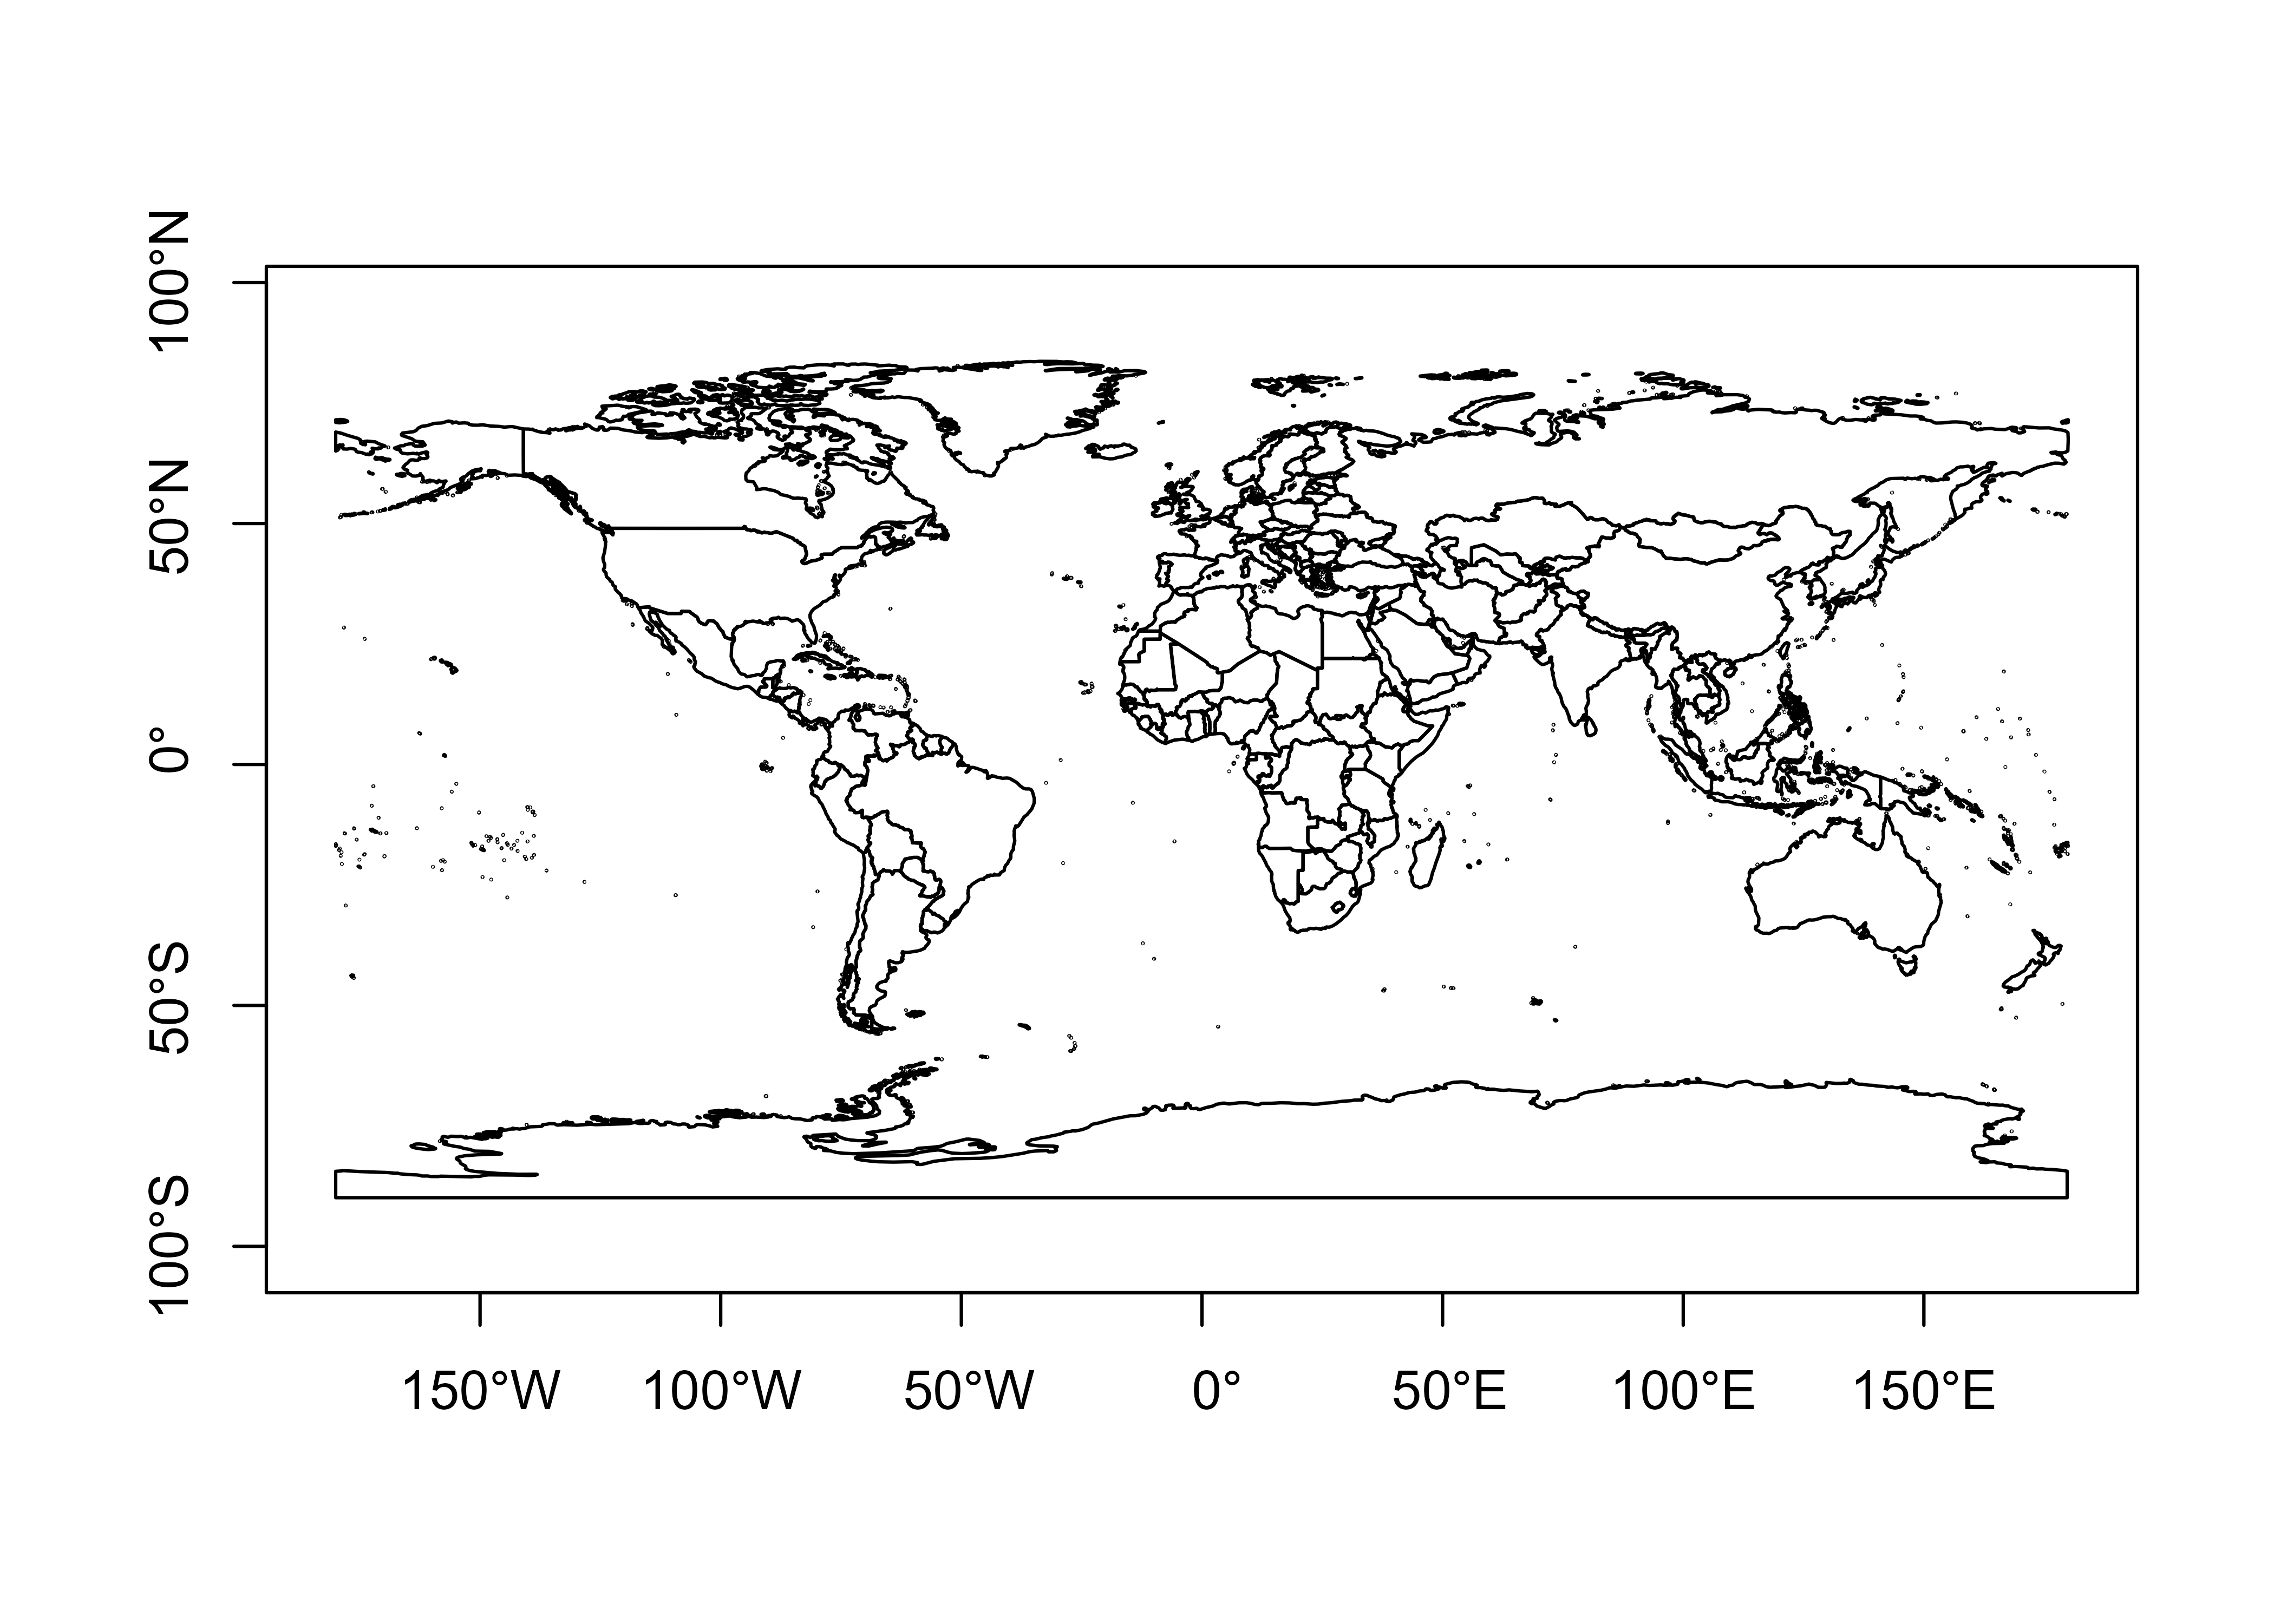
\includegraphics[width=0.6\linewidth]{_main_files/figure-latex/project-map-1} 

}

\caption{Proyección del mundo en coordenadas geográficas (EPSG 4326)}\label{fig:project-map-1}
\end{figure}

\begin{Shaded}
\begin{Highlighting}[]

\CommentTok{\# Proyectamos a Mercator}
\CommentTok{\# El eje cambia porque Mercator usa metros}
\NormalTok{paises\_merc }\OtherTok{\textless{}{-}} \FunctionTok{st\_transform}\NormalTok{(paises, }\FunctionTok{st\_crs}\NormalTok{(}\DecValTok{3857}\NormalTok{))}
\FunctionTok{plot}\NormalTok{(}\FunctionTok{st\_geometry}\NormalTok{(paises\_merc), }\AttributeTok{axes =} \ConstantTok{TRUE}\NormalTok{)}
\end{Highlighting}
\end{Shaded}

\begin{figure}

{\centering 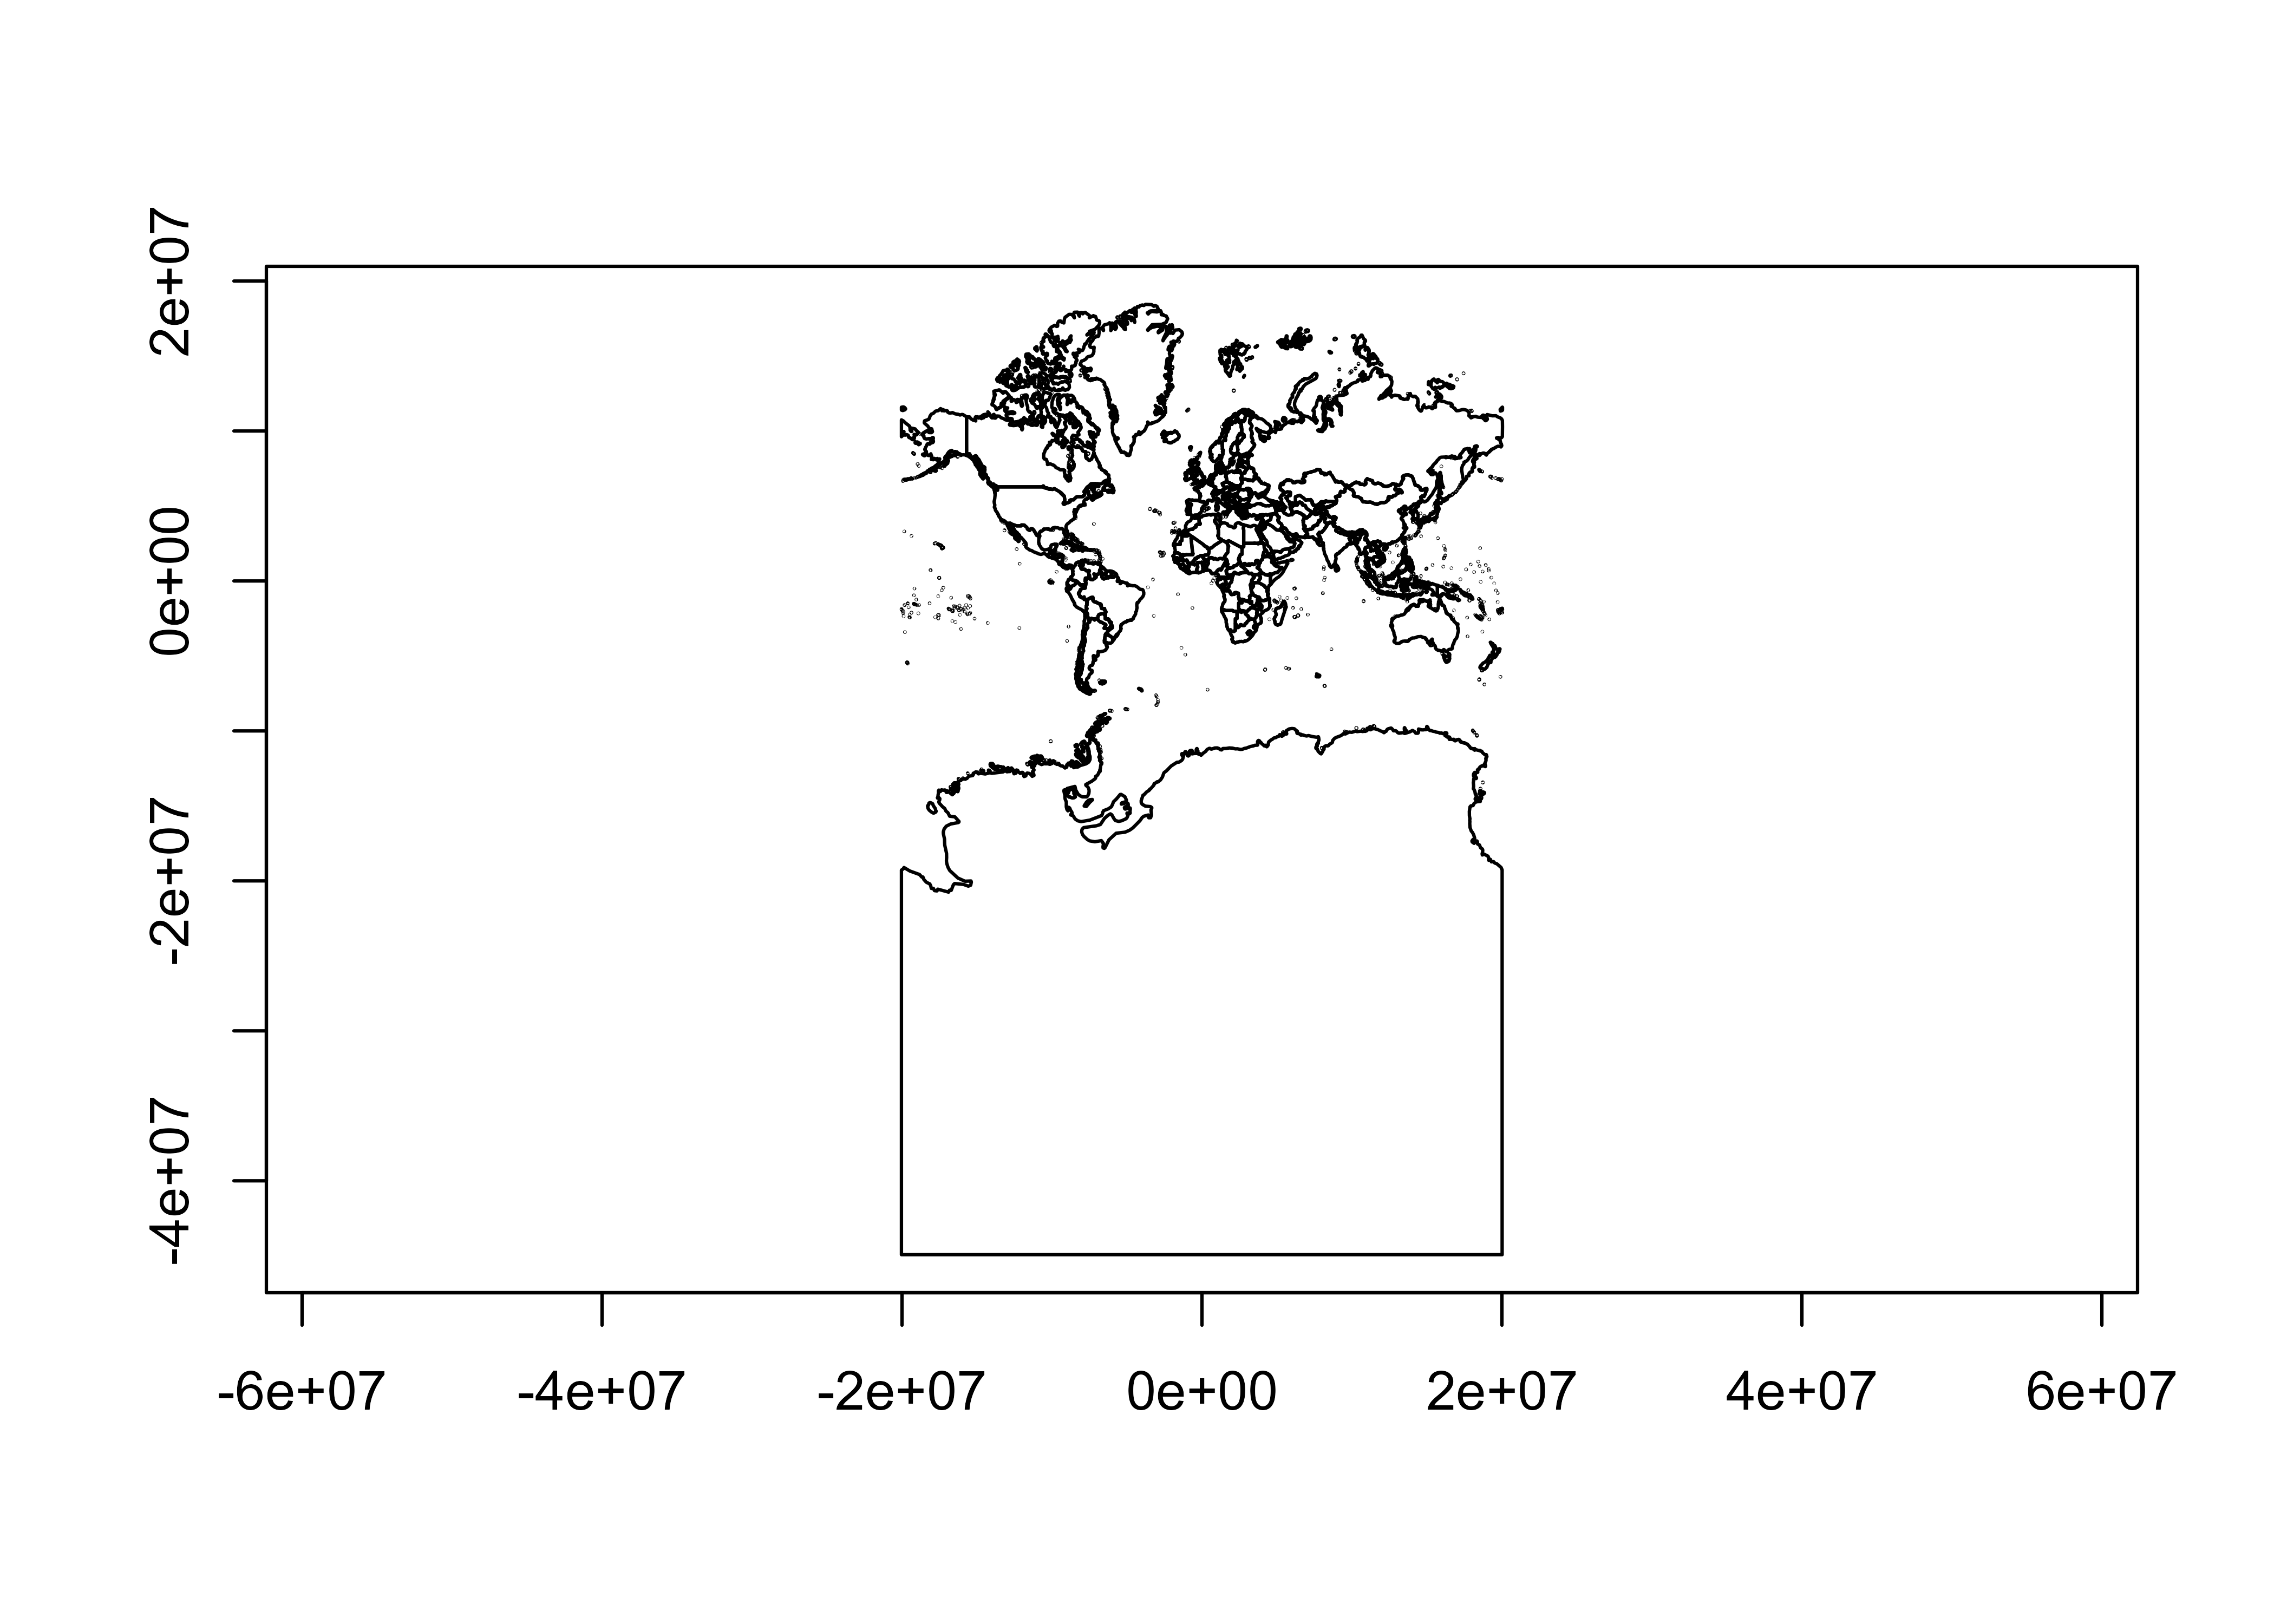
\includegraphics[width=0.6\linewidth]{_main_files/figure-latex/project-map-2} 

}

\caption{Proyección del mundo en Mercator (EPSG 3857)}\label{fig:project-map-2}
\end{figure}

\begin{Shaded}
\begin{Highlighting}[]
\CommentTok{\# Proyectamos a Robinson}
\NormalTok{paises\_robin }\OtherTok{\textless{}{-}} \FunctionTok{st\_transform}\NormalTok{(paises, }\FunctionTok{st\_crs}\NormalTok{(}\StringTok{"+proj=robin"}\NormalTok{))}
\FunctionTok{plot}\NormalTok{(}\FunctionTok{st\_geometry}\NormalTok{(paises\_robin), }\AttributeTok{axes =} \ConstantTok{TRUE}\NormalTok{)}
\end{Highlighting}
\end{Shaded}

\begin{figure}

{\centering 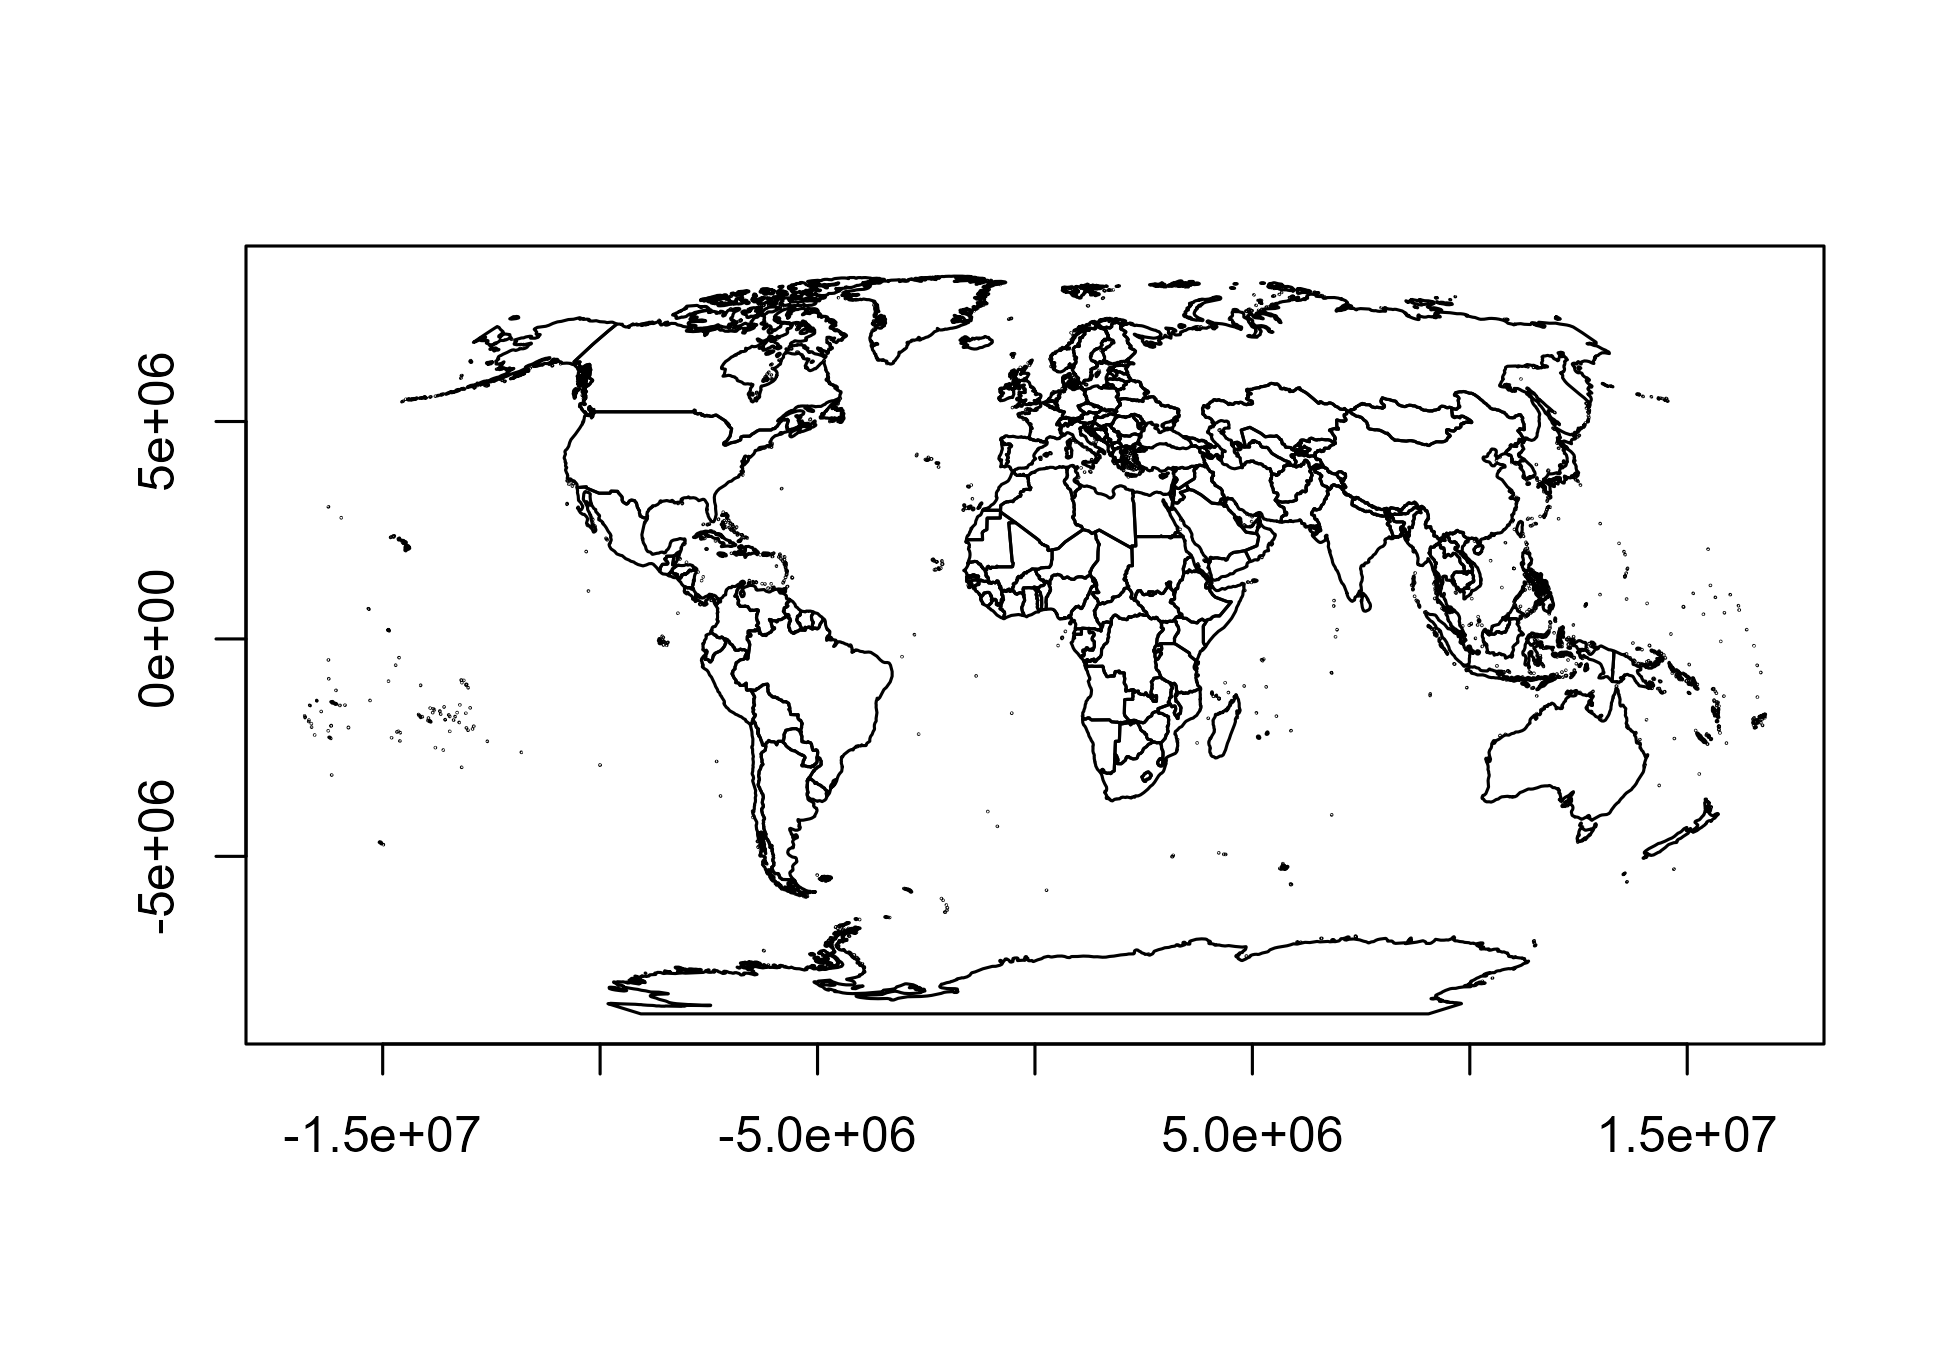
\includegraphics[width=0.6\linewidth]{_main_files/figure-latex/project-map-3} 

}

\caption{Proyección del mundo en Robinson (+proj=robin)}\label{fig:project-map-3}
\end{figure}

Como se comentó anteriormente, cuando se usan geodatos de diversas fuentes, es
necesario que todos presenten el mismo CRS. En la Fig \ref{fig:puertos-error}
se muestra lo que ocurre si esto no se cumple:

\begin{Shaded}
\begin{Highlighting}[]
\CommentTok{\# Añadimos a este mapa puertos mundiales de giscoR}

\NormalTok{puertos }\OtherTok{\textless{}{-}} \FunctionTok{gisco\_get\_ports}\NormalTok{()}
\FunctionTok{plot}\NormalTok{(}\FunctionTok{st\_geometry}\NormalTok{(paises\_robin), }\AttributeTok{main =} \StringTok{"Puertos en el mundo"}\NormalTok{)}
\FunctionTok{plot}\NormalTok{(}\FunctionTok{st\_geometry}\NormalTok{(puertos), }\AttributeTok{add =} \ConstantTok{TRUE}\NormalTok{, }\AttributeTok{col =} \StringTok{"red"}\NormalTok{, }\AttributeTok{pch =} \DecValTok{20}\NormalTok{)}
\end{Highlighting}
\end{Shaded}

\begin{figure}

{\centering 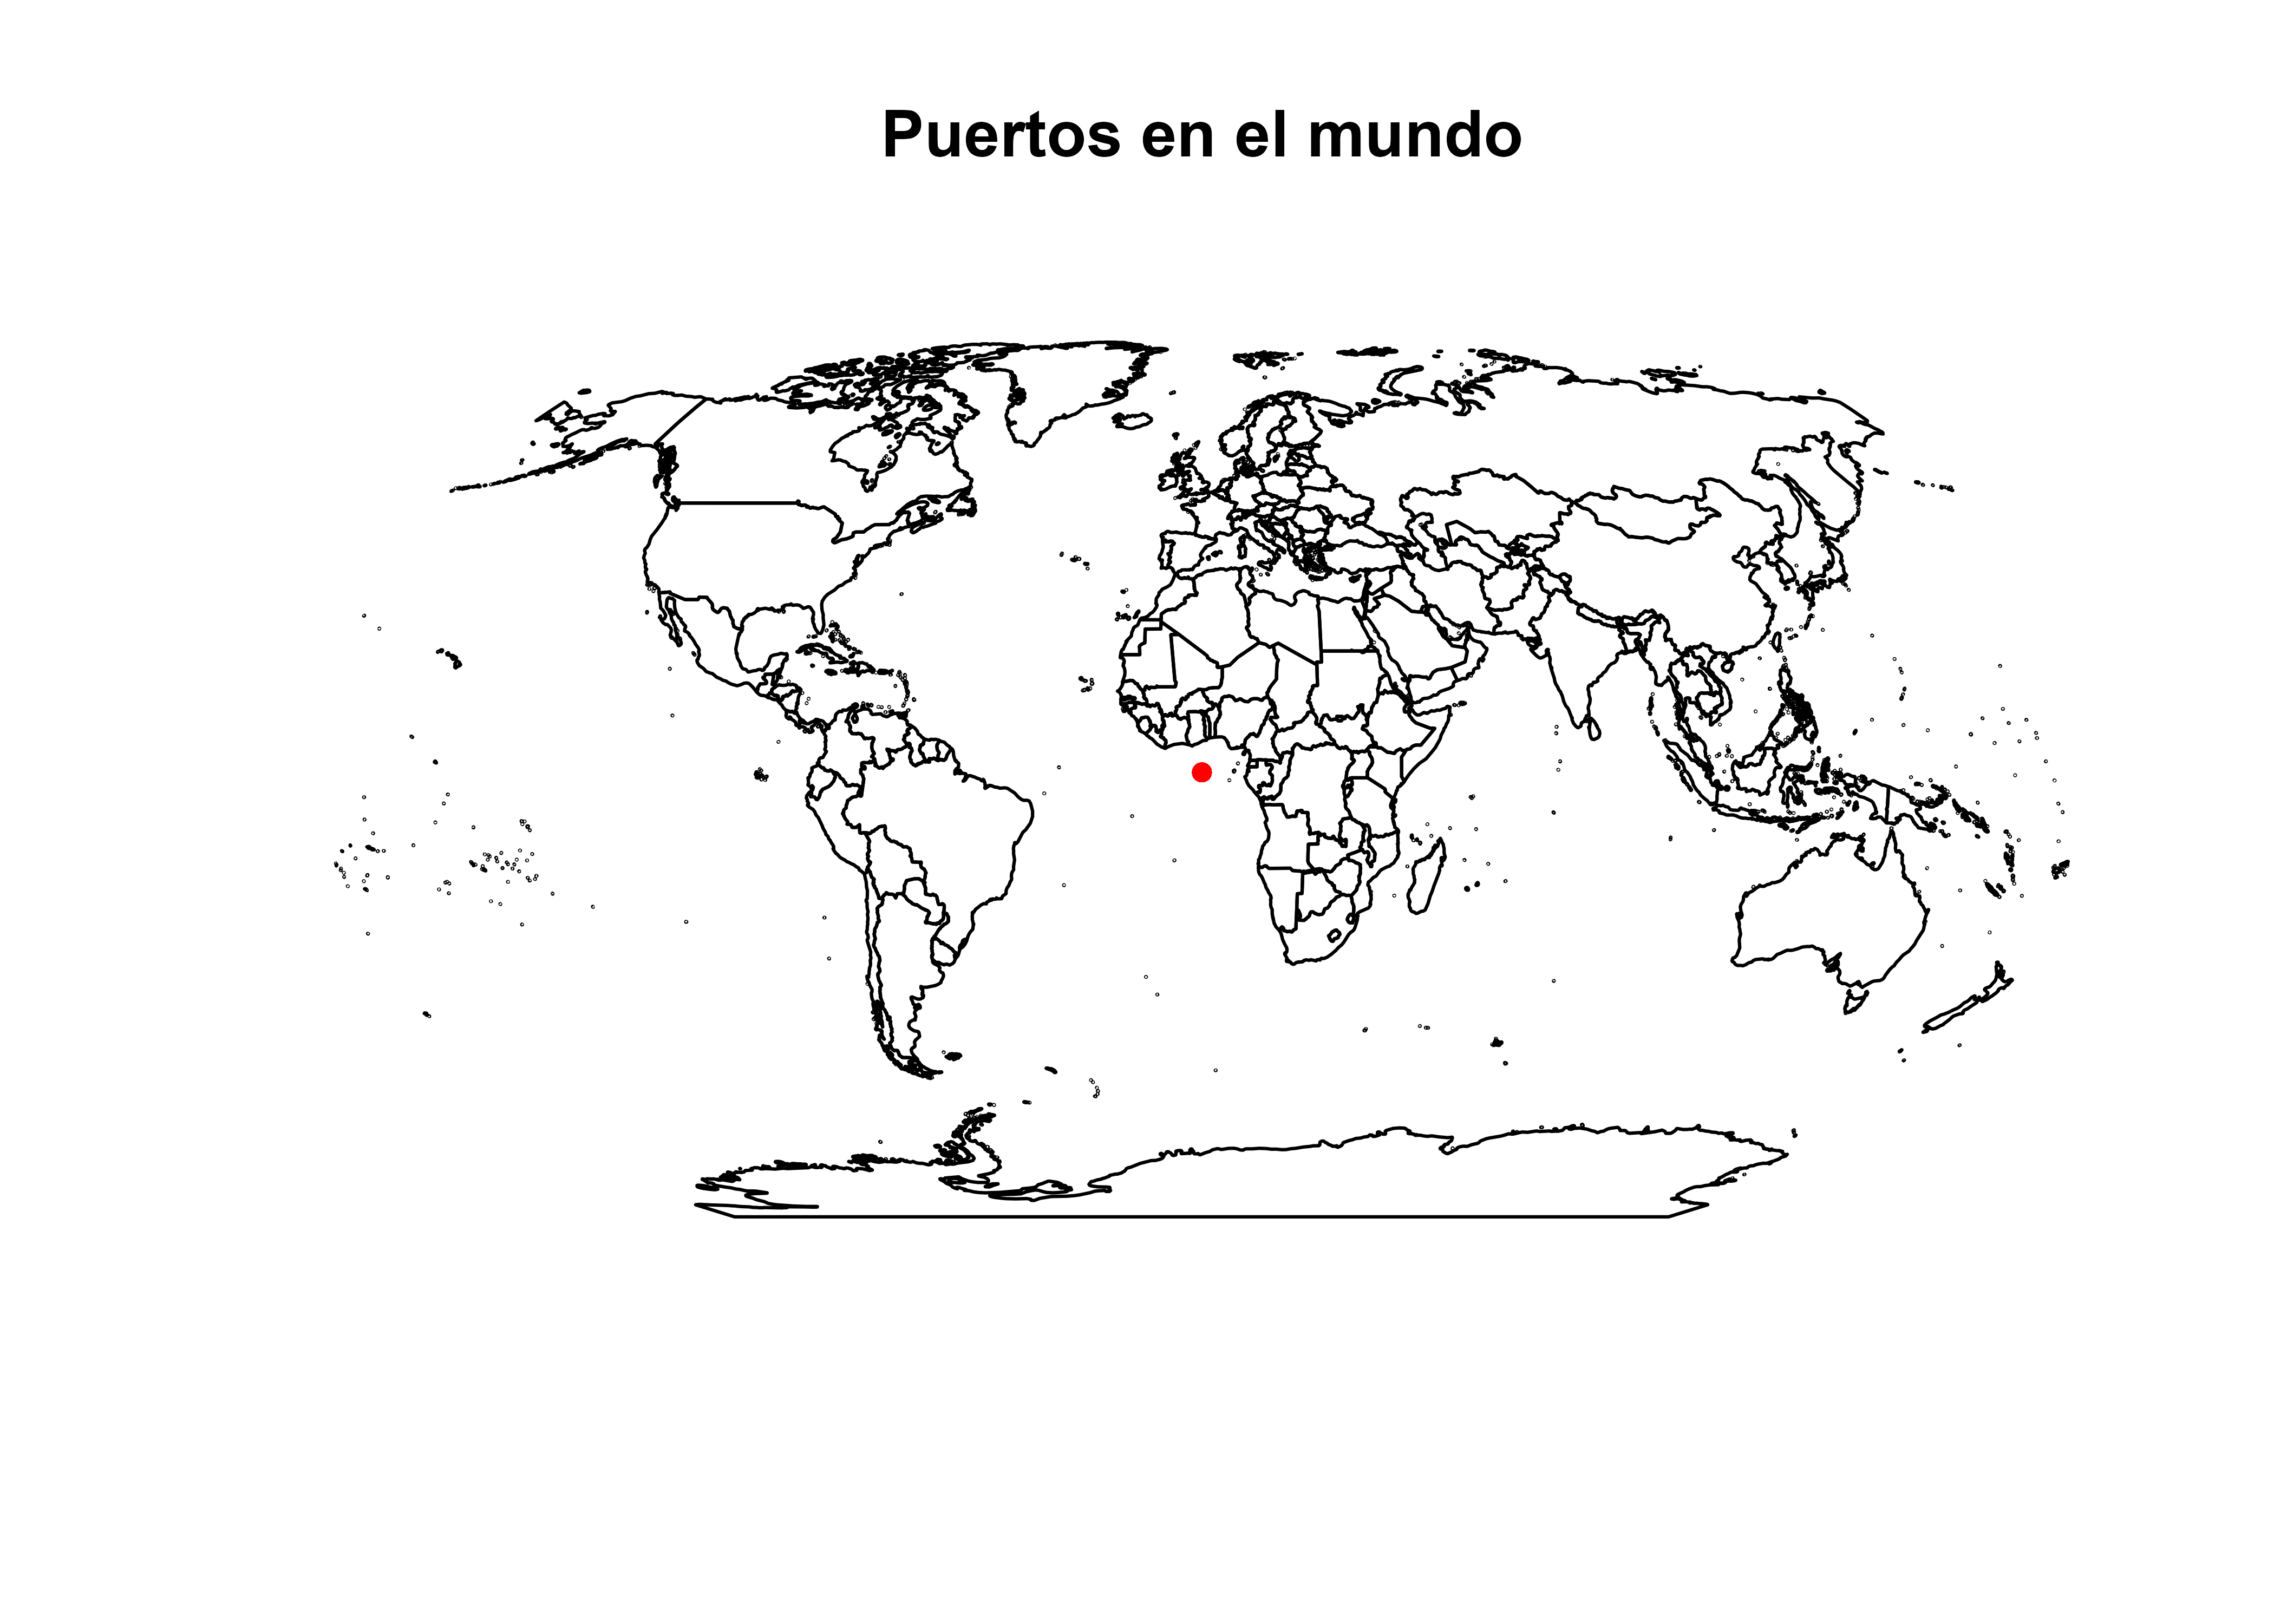
\includegraphics[width=0.6\linewidth]{_main_files/figure-latex/puertos-error-1} 

}

\caption{Ejemplo: Puertos del mundo}\label{fig:puertos-error}
\end{figure}

Vemos que ha habido algún tipo de error, ¿a que puede deberse?

\begin{Shaded}
\begin{Highlighting}[]
\CommentTok{\# Comprueba CRS}

\FunctionTok{st\_crs}\NormalTok{(puertos) }\SpecialCharTok{==} \FunctionTok{st\_crs}\NormalTok{(paises\_robin)}
\CommentTok{\#\textgreater{} [1] FALSE}

\CommentTok{\# Los puertos no están en Robinson! Proyectamos al mismo CRS}
\NormalTok{puertos\_robin }\OtherTok{\textless{}{-}} \FunctionTok{st\_transform}\NormalTok{(puertos, }\FunctionTok{st\_crs}\NormalTok{(paises\_robin))}
\FunctionTok{plot}\NormalTok{(}\FunctionTok{st\_geometry}\NormalTok{(paises\_robin), }\AttributeTok{main =} \StringTok{"Puertos en el mundo"}\NormalTok{)}
\FunctionTok{plot}\NormalTok{(}\FunctionTok{st\_geometry}\NormalTok{(puertos\_robin), }\AttributeTok{add =} \ConstantTok{TRUE}\NormalTok{, }\AttributeTok{col =} \StringTok{"blue"}\NormalTok{, }\AttributeTok{pch =} \DecValTok{20}\NormalTok{)}
\end{Highlighting}
\end{Shaded}

\begin{figure}

{\centering 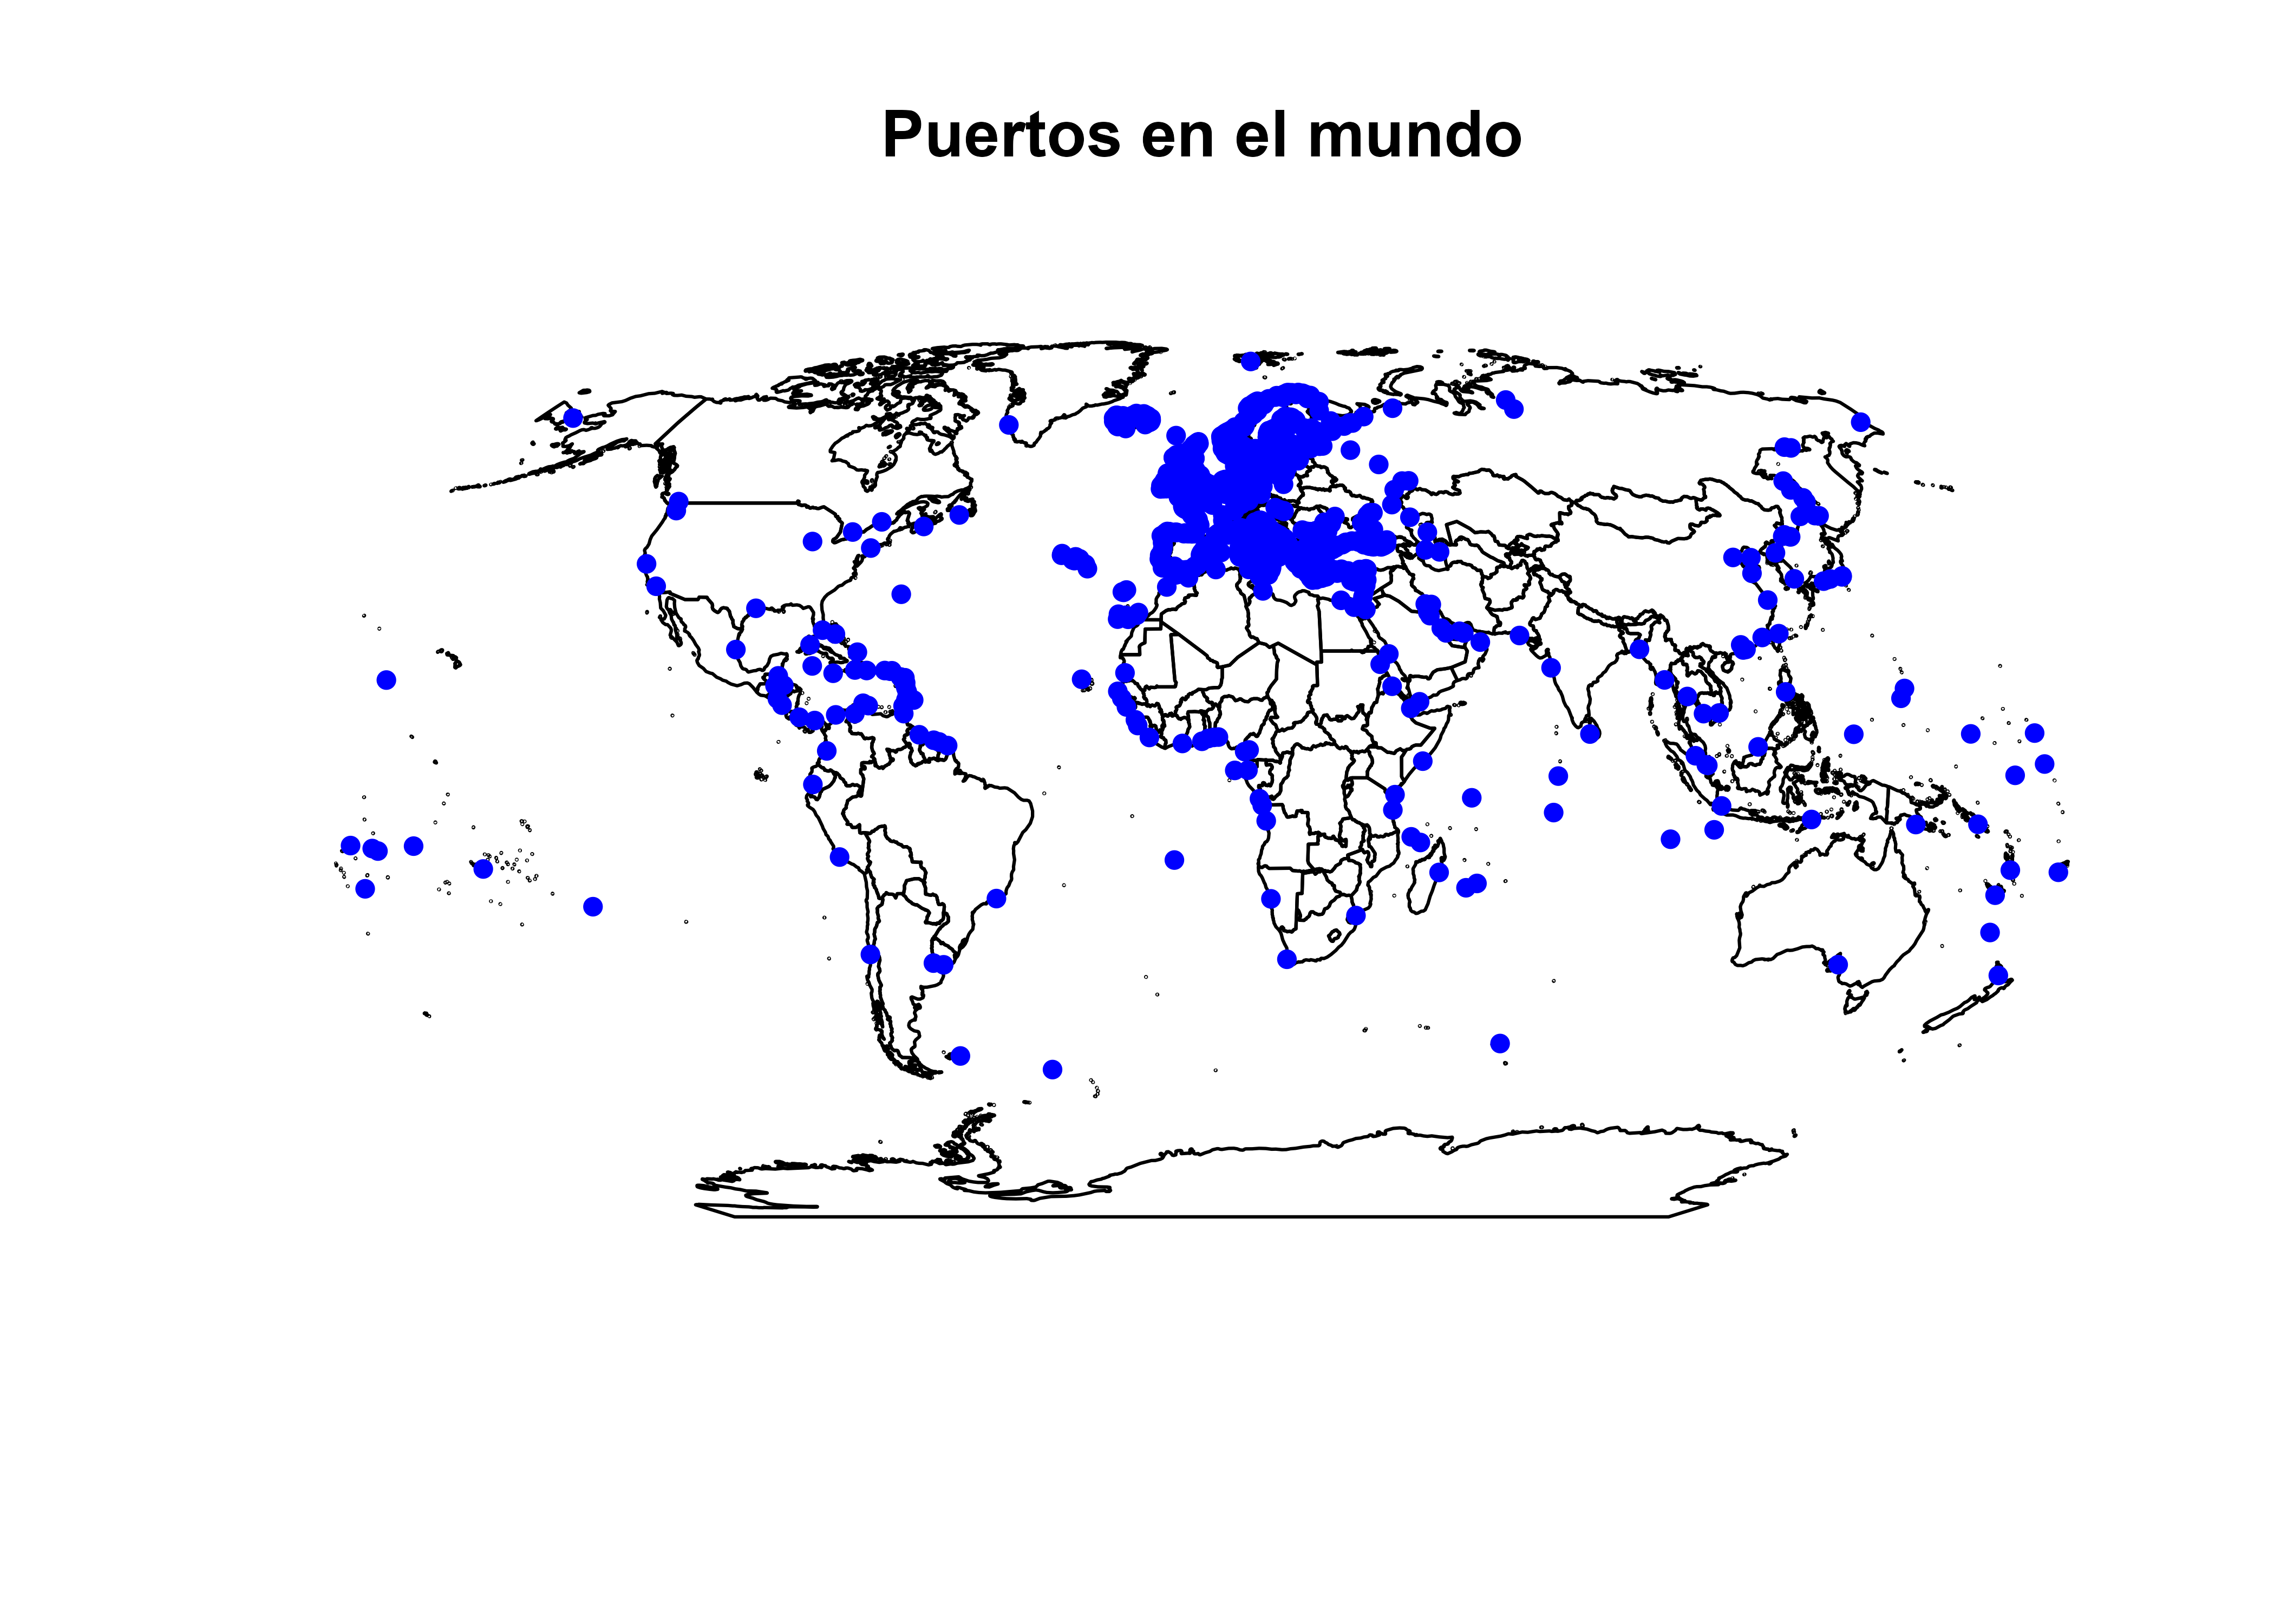
\includegraphics[width=0.6\linewidth]{_main_files/figure-latex/puertos-ok-1} 

}

\caption{Ejemplo: Puertos del mundo, CRS alineados}\label{fig:puertos-ok}
\end{figure}

Como vemos, en el primer mapa (Fig. \ref{fig:puertos-error}) los puertos se
concentran en un único punto, dado que no están referenciados en el mismo CRS.
Tras proyectarlos al mismo CRS, el mapa se representa adecuadamente (Fig.
\ref{fig:puertos-ok}).

En otros paquetes, como \texttt{sp} o \texttt{raster}, existen funciones parecidas que nos van
a permitir obtener los parámetros de un CRS y proyectar los objetos al CRS
deseado. Cuando empleemos el paquete \texttt{sp} podemos usar las funciones \texttt{CRS()} y
\texttt{spTransform()}:

\begin{Shaded}
\begin{Highlighting}[]

\FunctionTok{library}\NormalTok{(sp)}

\CommentTok{\# Convertimos sf a sp}
\NormalTok{paises\_sp }\OtherTok{\textless{}{-}} \FunctionTok{as}\NormalTok{(paises, }\StringTok{"Spatial"}\NormalTok{)}

\CommentTok{\# En sp podemos usar:}
\CommentTok{\# CRS("+proj=robin")}
\CommentTok{\#}
\CommentTok{\# O también desde sf}
\CommentTok{\# CRS(st\_crs(paises\_robin)$proj4string)}


\NormalTok{paises\_sp\_robin }\OtherTok{\textless{}{-}} \FunctionTok{spTransform}\NormalTok{(paises\_sp, }\FunctionTok{CRS}\NormalTok{(}\StringTok{"+proj=robin"}\NormalTok{))}
\FunctionTok{plot}\NormalTok{(paises\_sp\_robin)}
\end{Highlighting}
\end{Shaded}

\begin{figure}

{\centering 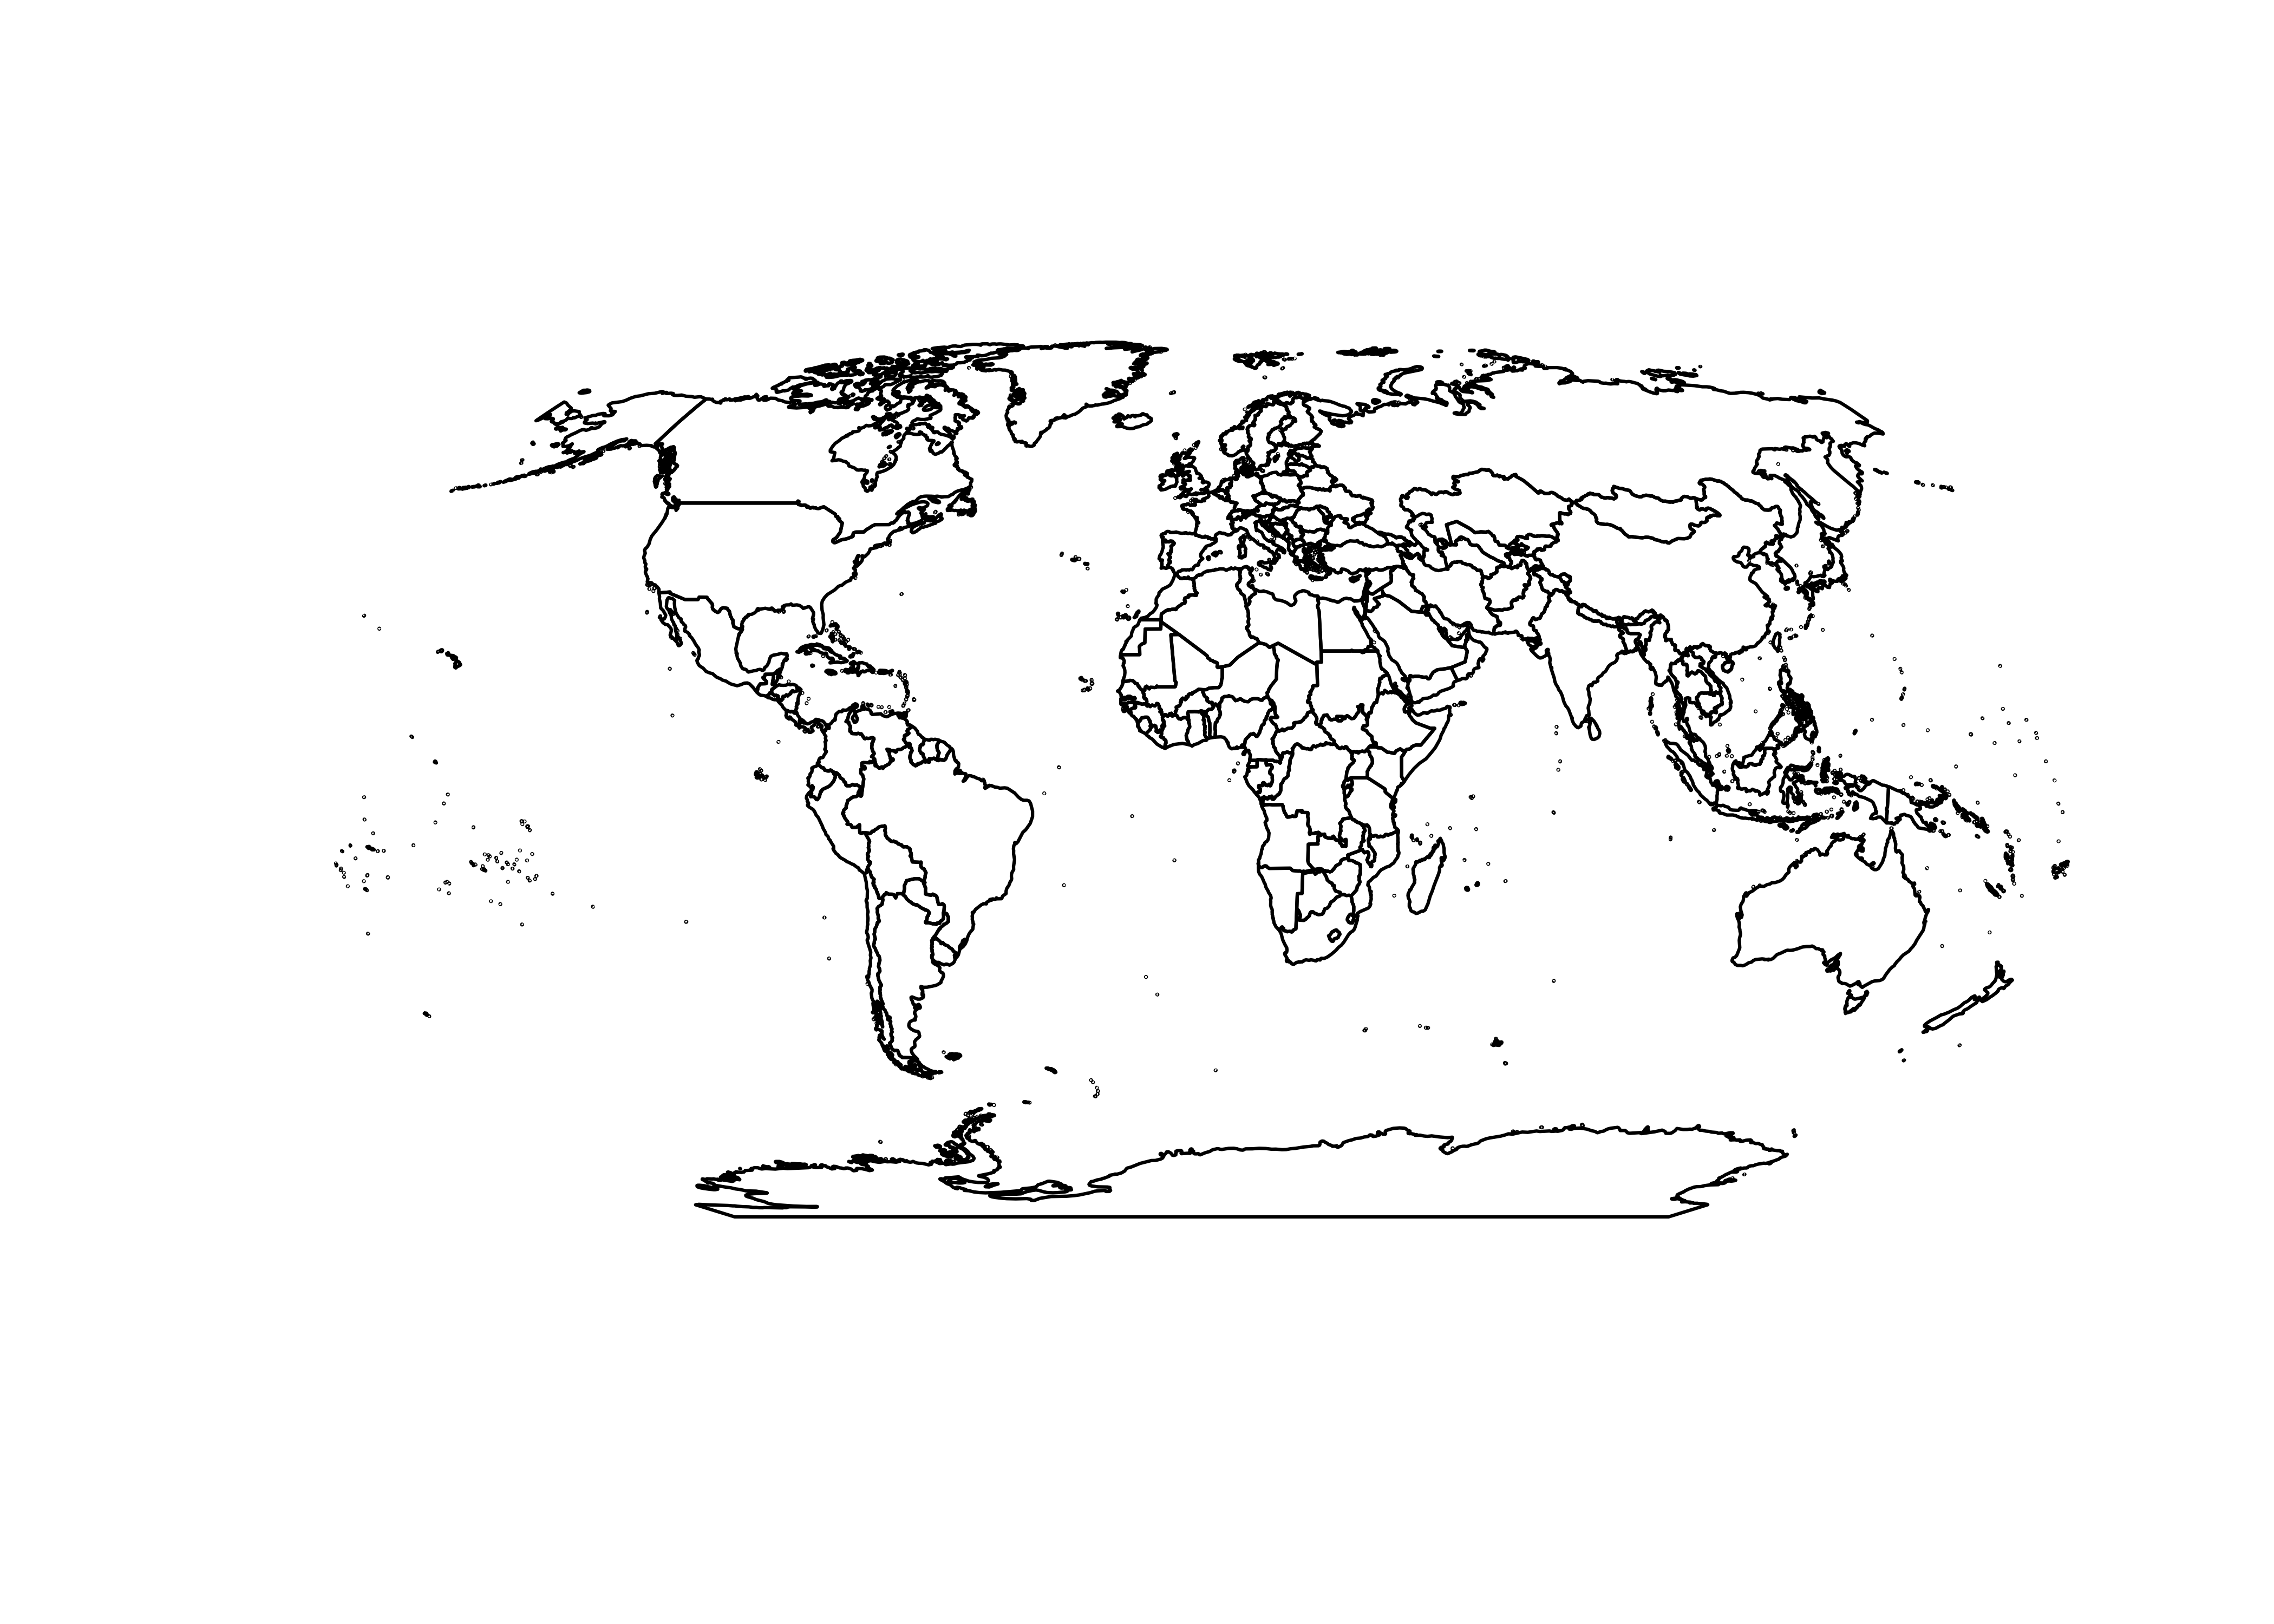
\includegraphics[width=0.6\linewidth]{_main_files/figure-latex/sp-1} 

}

\caption{Transformaciones en sp}\label{fig:sp}
\end{figure}

En el caso de un objeto \texttt{raster}, podemos usar \texttt{crs()} y \texttt{projectRaster()}:

\begin{Shaded}
\begin{Highlighting}[]
\FunctionTok{library}\NormalTok{(raster)}


\CommentTok{\# Extrae información de altitud para España}
\NormalTok{elev }\OtherTok{\textless{}{-}} \FunctionTok{raster}\NormalTok{(}\StringTok{"data/ESP\_msk\_alt.grd"}\NormalTok{)}


\CommentTok{\# Transforma}
\NormalTok{elev\_robinson }\OtherTok{\textless{}{-}} \FunctionTok{projectRaster}\NormalTok{(elev, }\AttributeTok{crs =} \FunctionTok{crs}\NormalTok{(}\StringTok{"+proj=robin"}\NormalTok{))}
\FunctionTok{plot}\NormalTok{(elev\_robinson)}
\end{Highlighting}
\end{Shaded}

\begin{figure}

{\centering 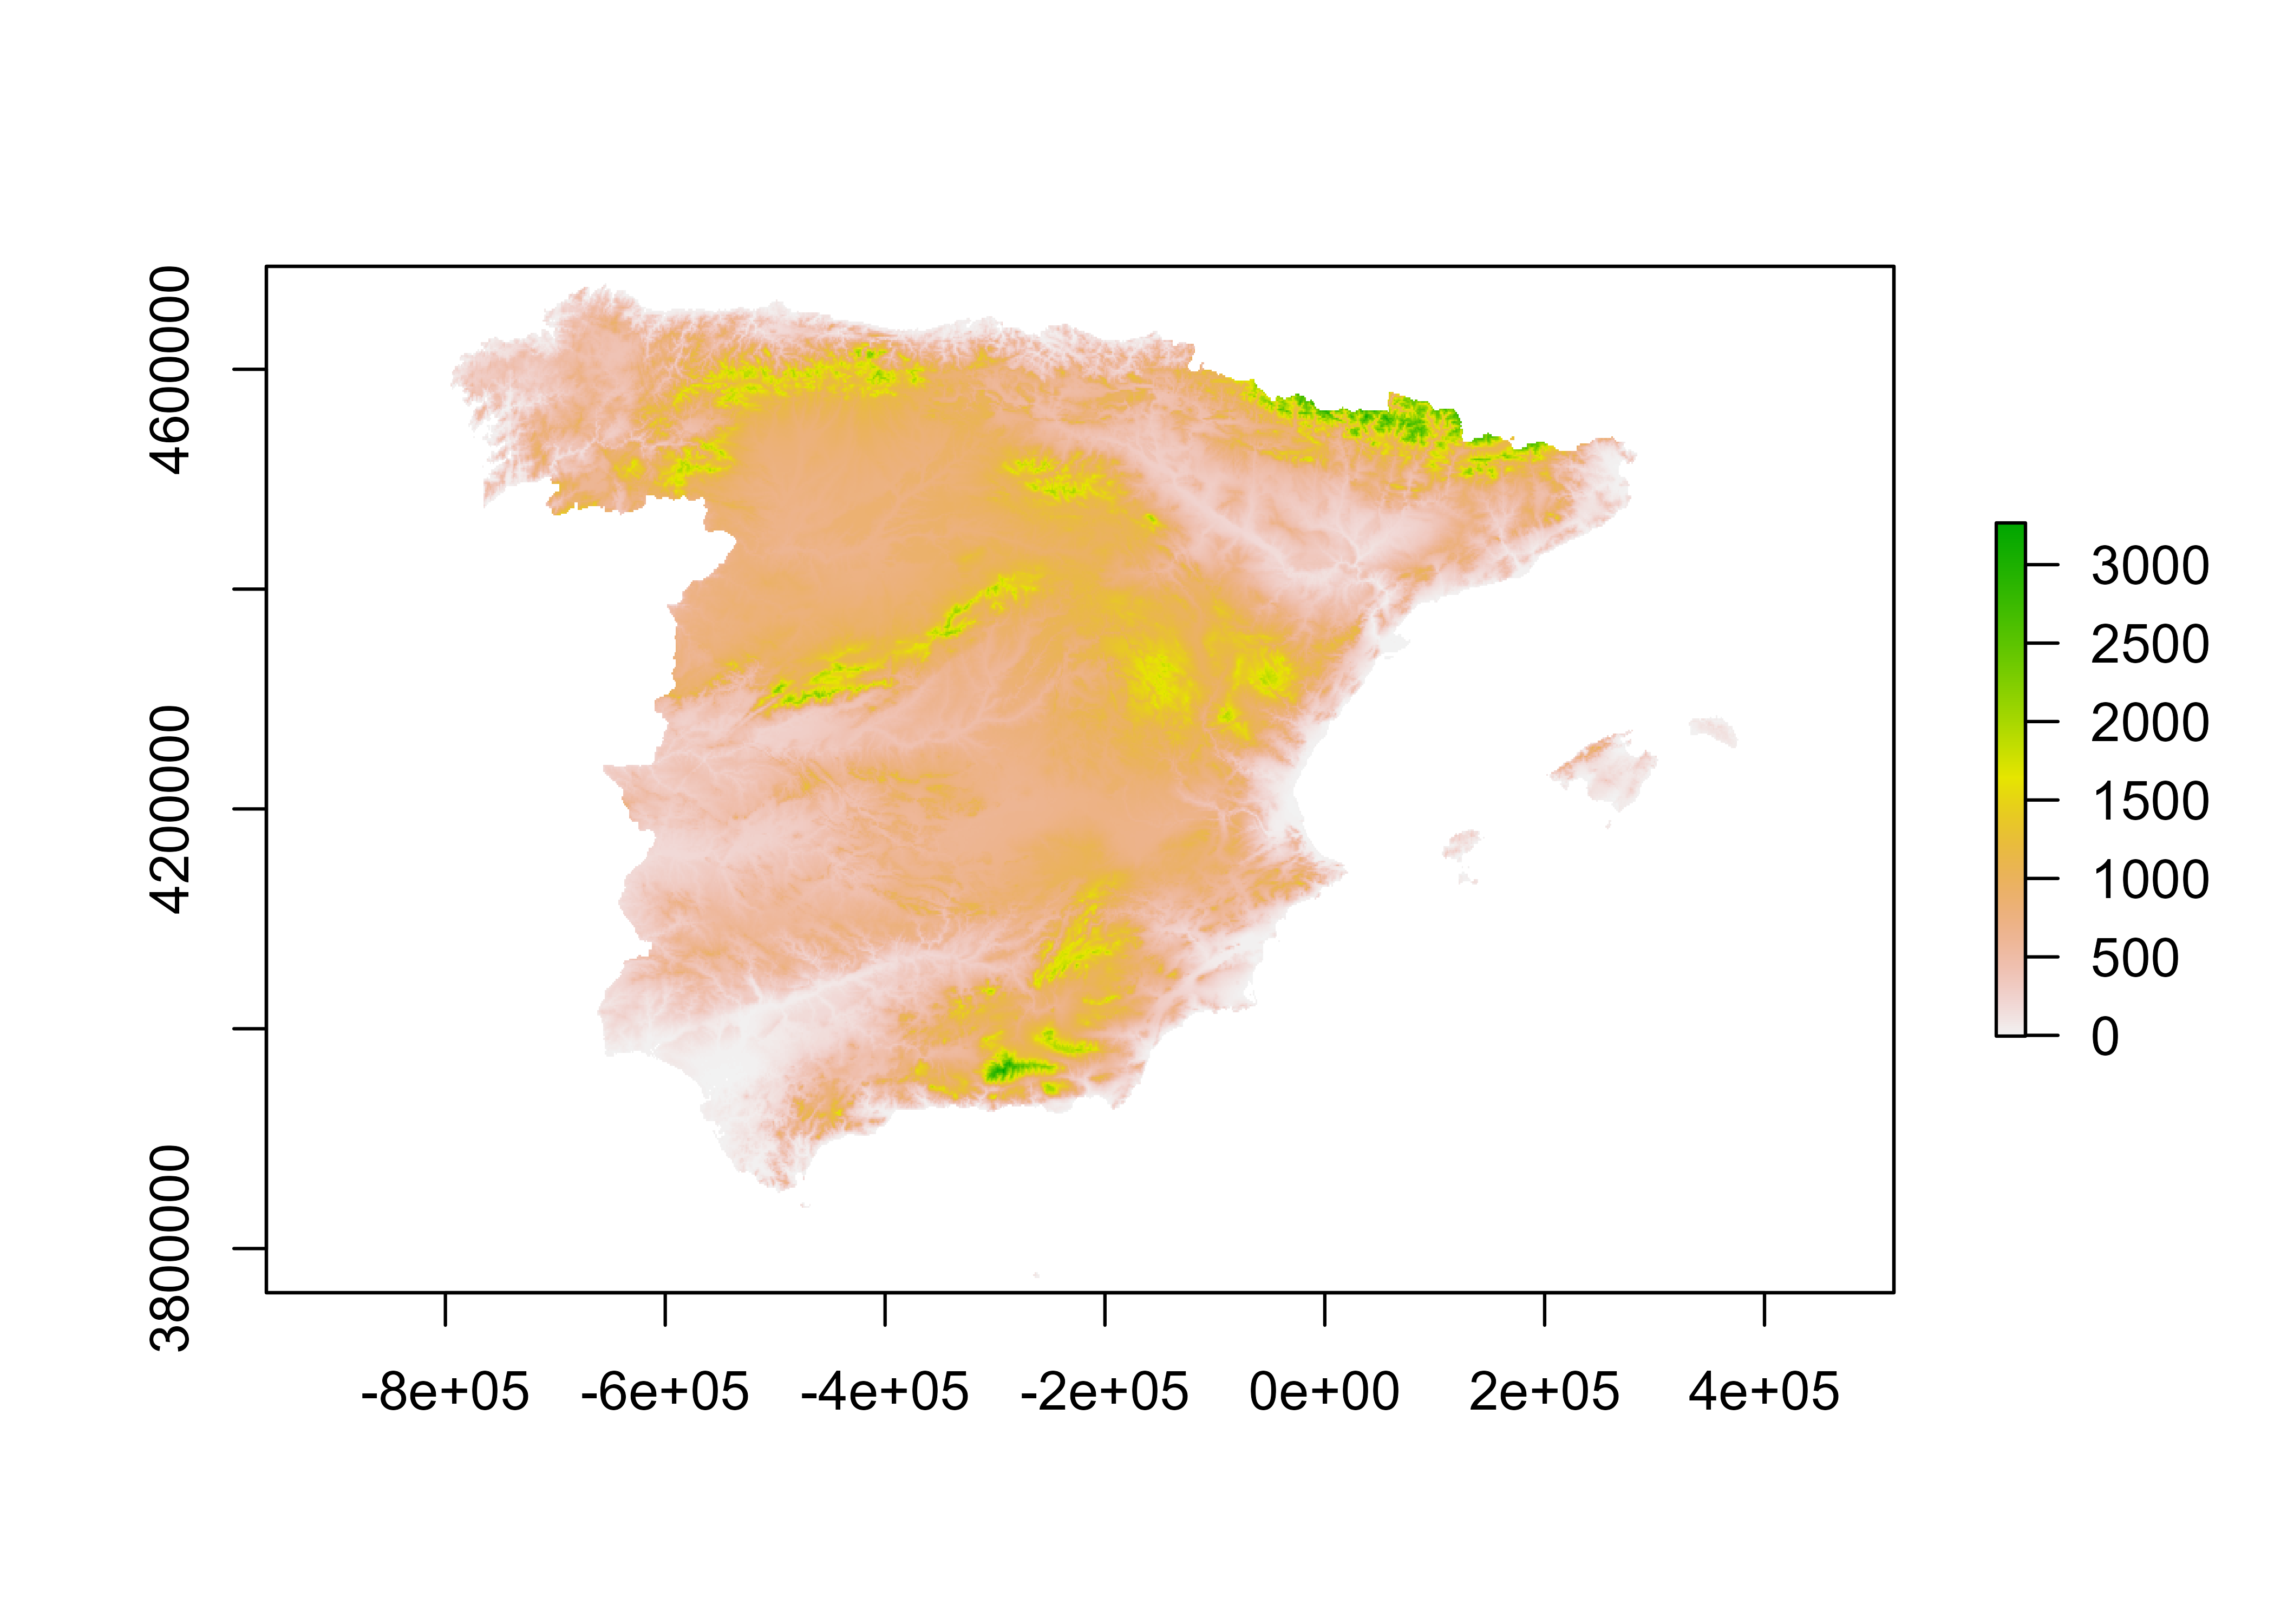
\includegraphics[width=0.6\linewidth]{_main_files/figure-latex/raster-crs-1} 

}

\caption{Transformaciones en raster}\label{fig:raster-crs}
\end{figure}

Por último, en el paquete \texttt{terra} las funciones correspondientes son \texttt{crs()} y
\texttt{project()}:

\begin{Shaded}
\begin{Highlighting}[]
\FunctionTok{library}\NormalTok{(terra)}

\CommentTok{\# Convierte de raster a terra}
\NormalTok{elev\_terra }\OtherTok{\textless{}{-}} \FunctionTok{rast}\NormalTok{(elev)}


\CommentTok{\# Transforma}
\NormalTok{elev\_terra\_robinson }\OtherTok{\textless{}{-}}\NormalTok{ terra}\SpecialCharTok{::}\FunctionTok{project}\NormalTok{(elev\_terra, terra}\SpecialCharTok{::}\FunctionTok{crs}\NormalTok{(elev\_terra))}
\FunctionTok{plot}\NormalTok{(elev\_terra\_robinson)}
\end{Highlighting}
\end{Shaded}

\begin{figure}

{\centering 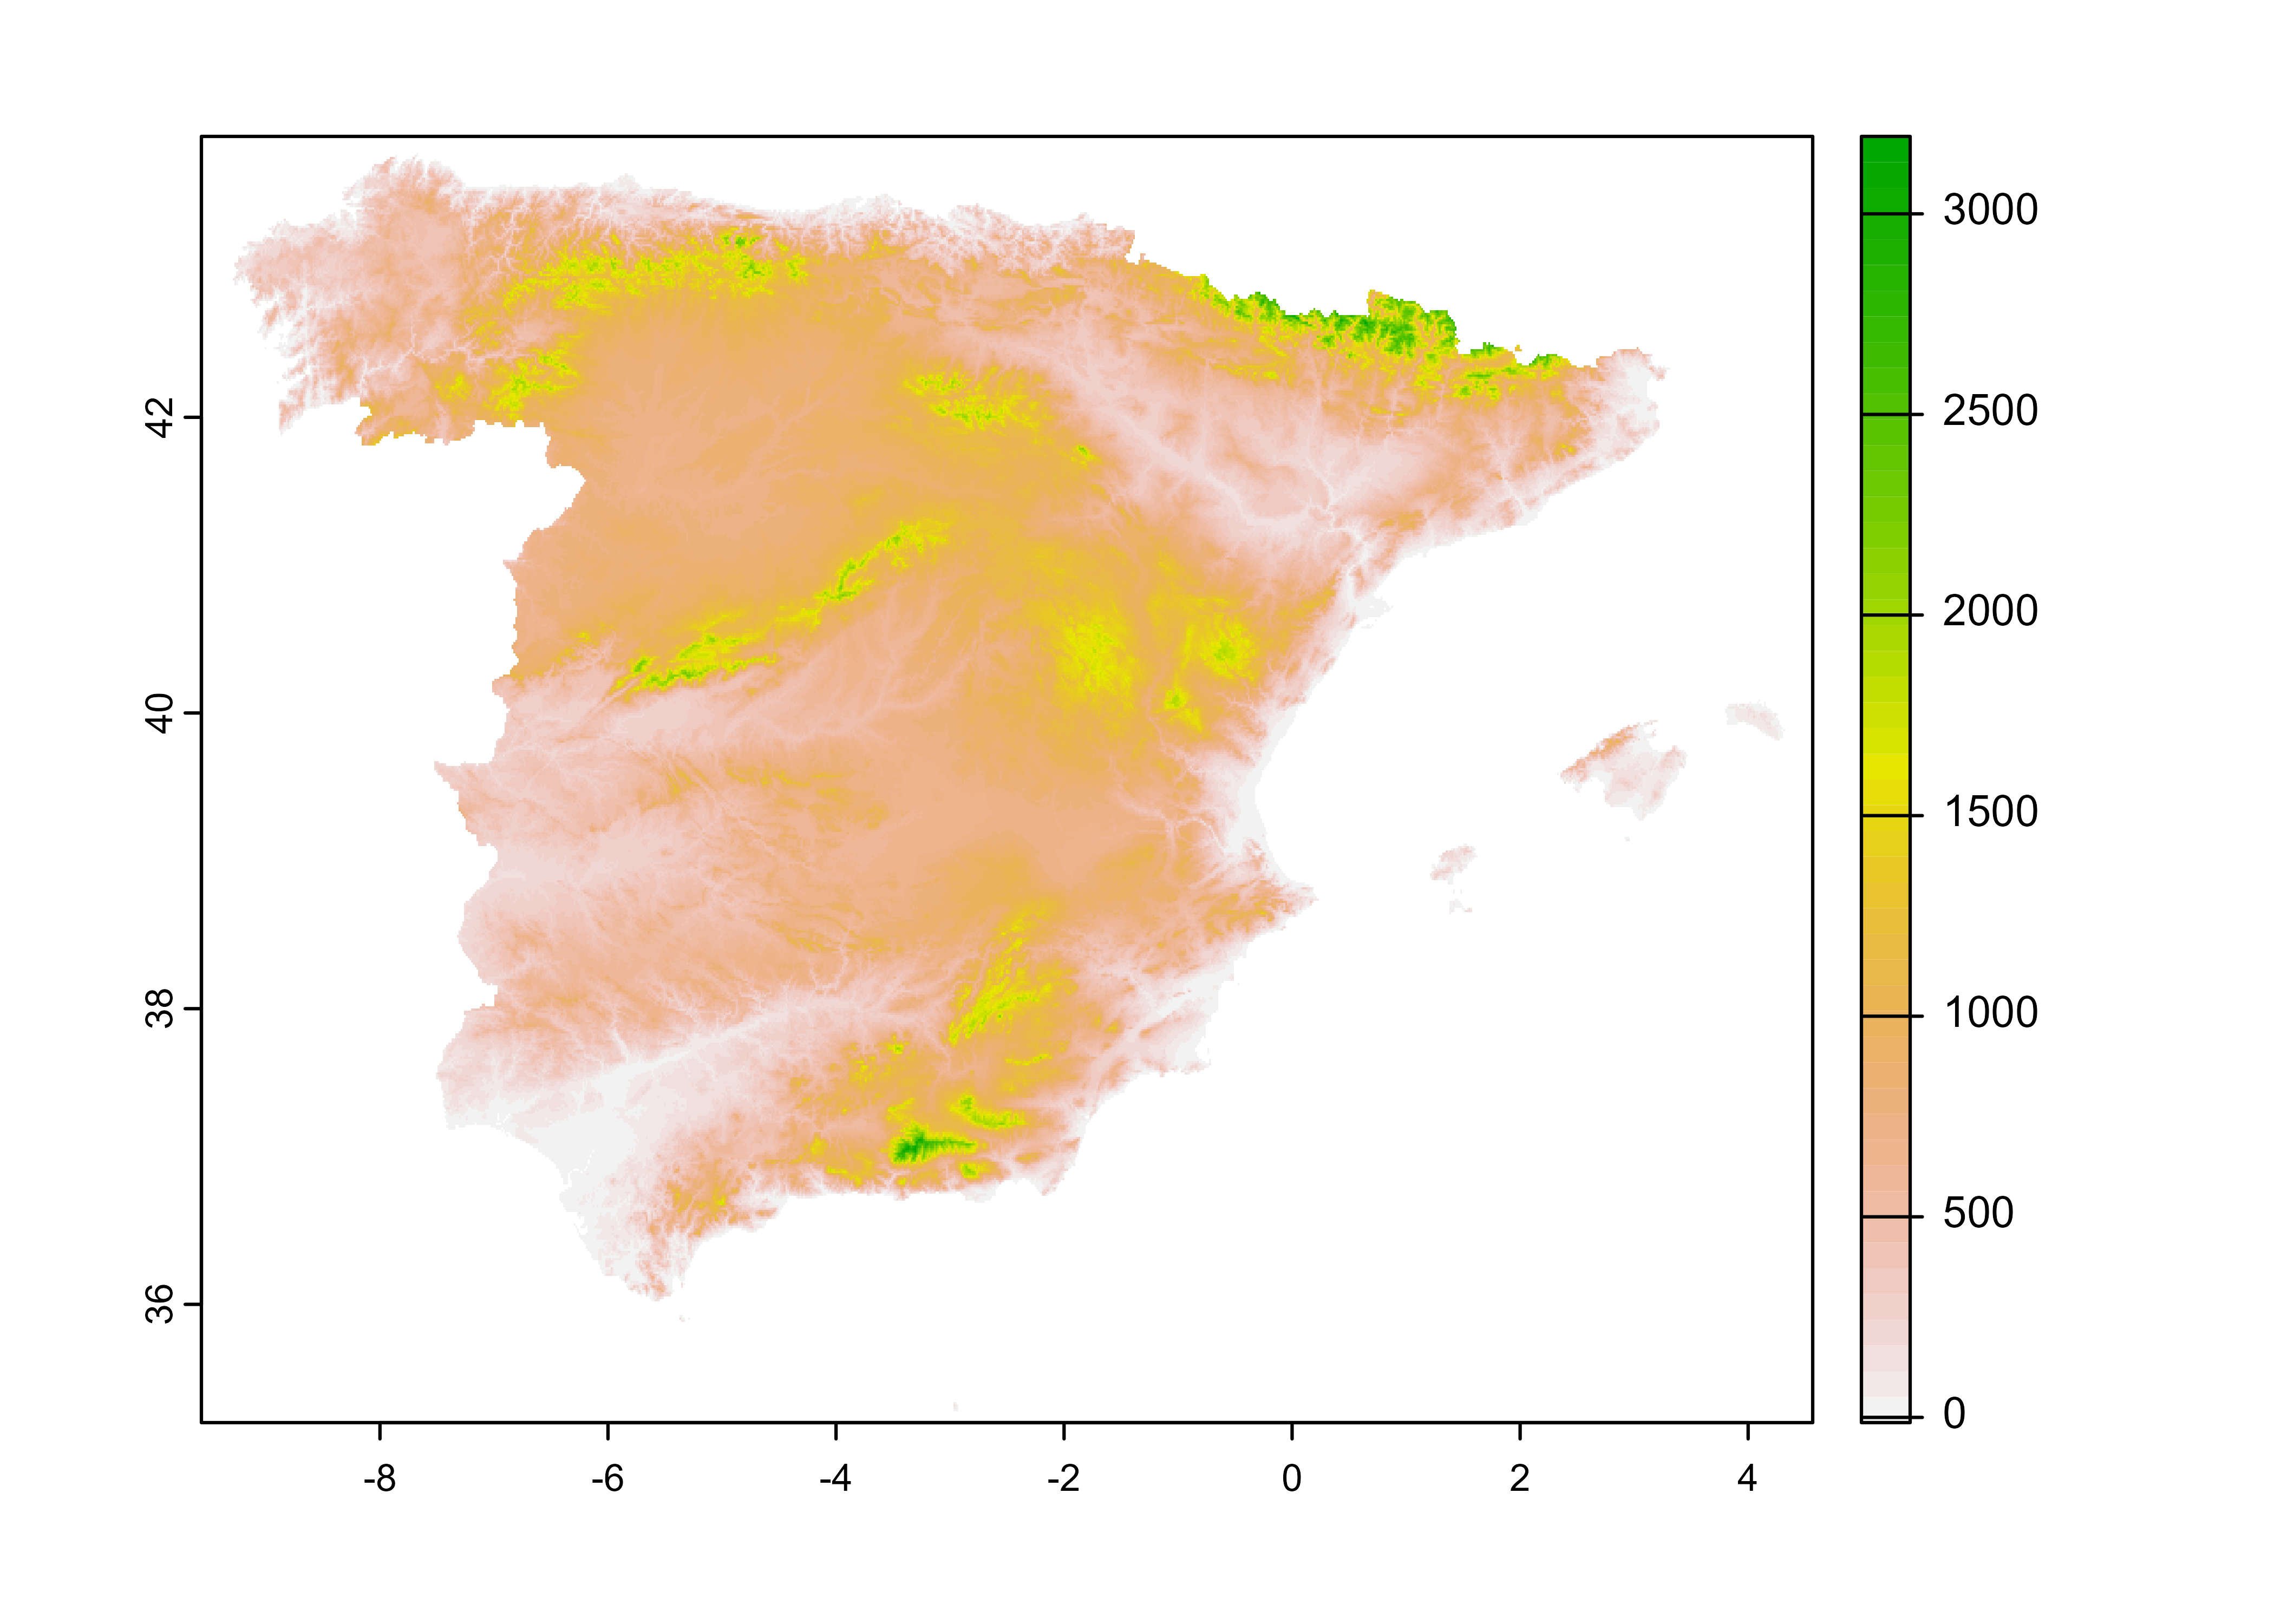
\includegraphics[width=0.6\linewidth]{_main_files/figure-latex/terra-1} 

}

\caption{Transformaciones en terra}\label{fig:terra}
\end{figure}

\hypertarget{quecrsuso}{%
\subsection{¿Qué proyección uso?}\label{quecrsuso}}

El CRS adecuado para cada análisis depende de la localización y el rango
espacial de los datos. Un CRS adecuado para representar un mapa del mundo puede
no serlo para representar datos de zonas específicas de la Tierra. Los recursos
web mencionados anteriormente permiten la búsqueda de CRS por zona geográfica, y
adicionalmente en \textbf{R} existe el paquete \texttt{crsuggest} \citep{R-crsuggest} que nos
facilita la labor, sugiriendo el CRS más adecuado para cada zona:

\begin{Shaded}
\begin{Highlighting}[]
\FunctionTok{library}\NormalTok{(crsuggest)}

\CommentTok{\# Usando raster}
\NormalTok{sugerencias }\OtherTok{\textless{}{-}} \FunctionTok{suggest\_crs}\NormalTok{(elev)}
\end{Highlighting}
\end{Shaded}

\begin{table}

\caption{\label{tab:muestra-tabla}Tabla sugerencias, detalle}
\centering
\begin{tabular}[t]{l|l|l|r|l|l}
\hline
crs\_code & crs\_name & crs\_type & crs\_gcs & crs\_units & crs\_proj4\\
\hline
2062 & Madrid 1870 (Madrid) / Spain LCC & projected & 4903 & m & +proj=lcc +lat\_1=40 +lat\_0=40 +lon\_0=0 +k\_0=0.9988085293 +x\_0=600000 +y\_0=600000 +a=6378298.3 +rf=294.73 +pm=madrid +units=m +no\_defs\\
\hline
2154 & RGF93 / Lambert-93 & projected & 4171 & m & +proj=lcc +lat\_0=46.5 +lon\_0=3 +lat\_1=49 +lat\_2=44 +x\_0=700000 +y\_0=6600000 +ellps=GRS80 +towgs84=0,0,0,0,0,0,0 +units=m +no\_defs\\
\hline
26191 & Merchich / Nord Maroc & projected & 4261 & m & +proj=lcc +lat\_1=33.3 +lat\_0=33.3 +lon\_0=-5.4 +k\_0=0.999625769 +x\_0=500000 +y\_0=300000 +ellps=clrk80ign +towgs84=31,146,47,0,0,0,0 +units=m +no\_defs\\
\hline
3944 & RGF93 / CC44 & projected & 4171 & m & +proj=lcc +lat\_0=44 +lon\_0=3 +lat\_1=43.25 +lat\_2=44.75 +x\_0=1700000 +y\_0=3200000 +ellps=GRS80 +towgs84=0,0,0,0,0,0,0 +units=m +no\_defs\\
\hline
3943 & RGF93 / CC43 & projected & 4171 & m & +proj=lcc +lat\_0=43 +lon\_0=3 +lat\_1=42.25 +lat\_2=43.75 +x\_0=1700000 +y\_0=2200000 +ellps=GRS80 +towgs84=0,0,0,0,0,0,0 +units=m +no\_defs\\
\hline
27573 & NTF (Paris) / Lambert zone III & projected & 4807 & m & +proj=lcc +lat\_1=44.1 +lat\_0=44.1 +lon\_0=0 +k\_0=0.999877499 +x\_0=600000 +y\_0=3200000 +ellps=clrk80ign +pm=paris +towgs84=-168,-60,320,0,0,0,0 +units=m +no\_defs\\
\hline
27572 & NTF (Paris) / Lambert zone II & projected & 4807 & m & +proj=lcc +lat\_1=46.8 +lat\_0=46.8 +lon\_0=0 +k\_0=0.99987742 +x\_0=600000 +y\_0=2200000 +ellps=clrk80ign +pm=paris +towgs84=-168,-60,320,0,0,0,0 +units=m +no\_defs\\
\hline
27563 & NTF (Paris) / Lambert Sud France & projected & 4807 & m & +proj=lcc +lat\_1=44.1 +lat\_0=44.1 +lon\_0=0 +k\_0=0.999877499 +x\_0=600000 +y\_0=200000 +ellps=clrk80ign +pm=paris +towgs84=-168,-60,320,0,0,0,0 +units=m +no\_defs\\
\hline
30791 & Nord Sahara 1959 / Nord Algerie & projected & 4307 & m & +proj=lcc +lat\_1=36 +lat\_0=36 +lon\_0=2.7 +k\_0=0.999625544 +x\_0=500135 +y\_0=300090 +a=6378249.145 +rf=293.465 +towgs84=-209.3622,-87.8162,404.6198,0.0046,3.4784,0.5805,-1.4547 +units=m +no\_defs\\
\hline
30493 & Voirol 1879 / Nord Algerie (ancienne) & projected & 4671 & m & +proj=lcc +lat\_1=36 +lat\_0=36 +lon\_0=2.7 +k\_0=0.999625544 +x\_0=500000 +y\_0=300000 +ellps=clrk80ign +units=m +no\_defs\\
\hline
\end{tabular}
\end{table}

\begin{Shaded}
\begin{Highlighting}[]
\CommentTok{\# Probamos sugerencia}
\NormalTok{crs\_suggest }\OtherTok{\textless{}{-}} \FunctionTok{suggest\_crs}\NormalTok{(elev, }\AttributeTok{limit =} \DecValTok{1}\NormalTok{)}

\NormalTok{elev\_suggest }\OtherTok{\textless{}{-}} \FunctionTok{projectRaster}\NormalTok{(elev, }\AttributeTok{crs =}\NormalTok{ raster}\SpecialCharTok{::}\FunctionTok{crs}\NormalTok{(crs\_suggest}\SpecialCharTok{$}\NormalTok{crs\_proj4))}

\FunctionTok{plot}\NormalTok{(elev\_suggest)}
\end{Highlighting}
\end{Shaded}

\begin{figure}

{\centering 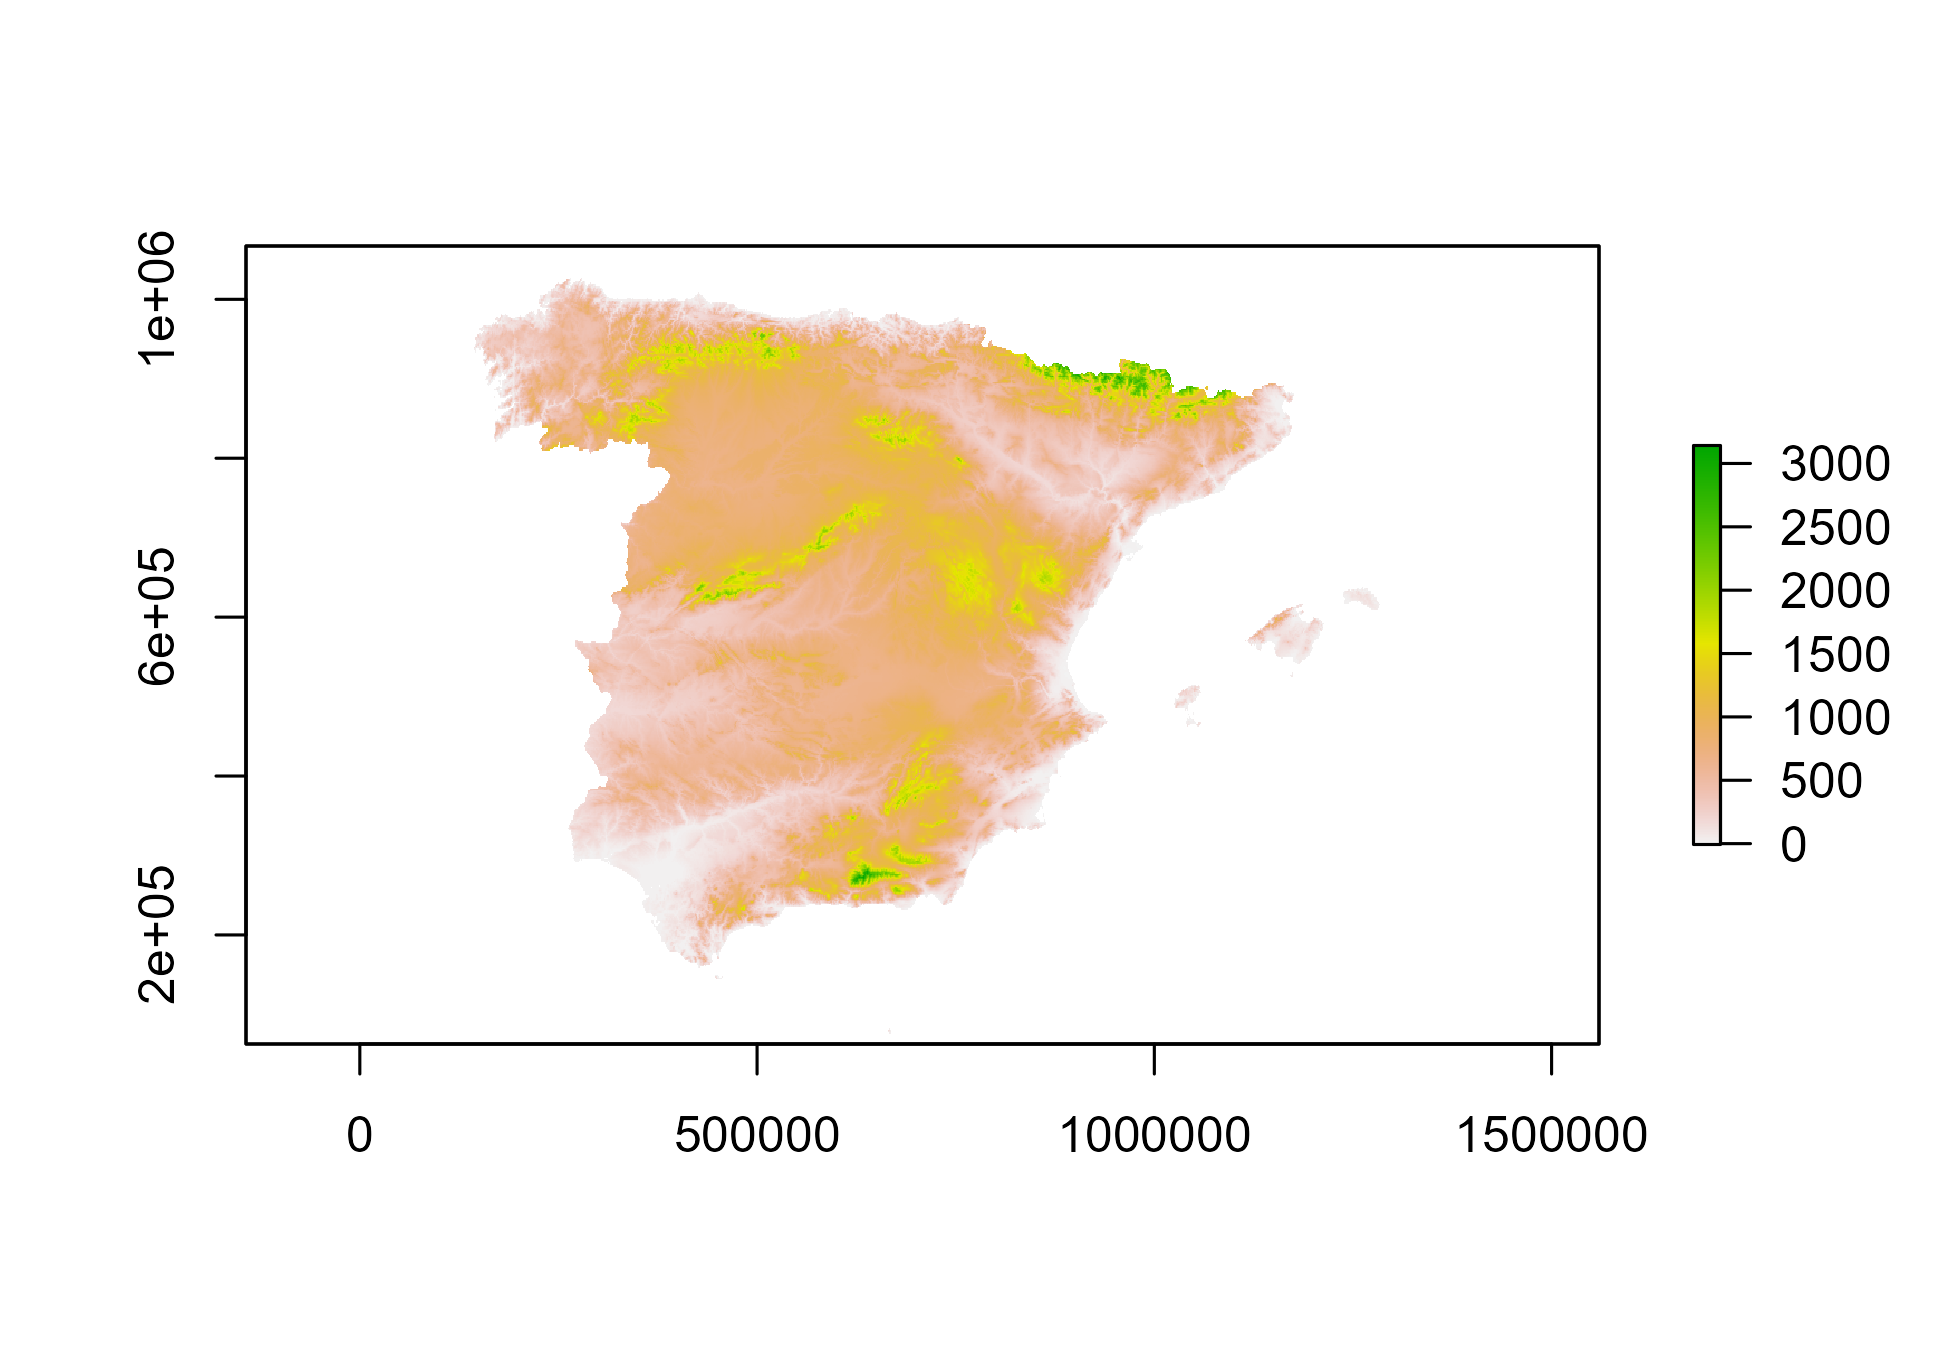
\includegraphics[width=0.6\linewidth]{_main_files/figure-latex/sugerencia-1} 

}

\caption{raster: Ejemplo de transformación usando crsuggest}\label{fig:sugerencia-1}
\end{figure}

\begin{Shaded}
\begin{Highlighting}[]

\CommentTok{\# Ejemplo con sf: China}

\NormalTok{china }\OtherTok{\textless{}{-}} \FunctionTok{gisco\_get\_countries}\NormalTok{(}\AttributeTok{country =} \StringTok{"China"}\NormalTok{)}
\NormalTok{china\_crs }\OtherTok{\textless{}{-}} \FunctionTok{suggest\_crs}\NormalTok{(china, }\AttributeTok{limit =} \DecValTok{1}\NormalTok{)}

\NormalTok{china\_crs}
\CommentTok{\#\textgreater{} \# A tibble: 1 x 6}
\CommentTok{\#\textgreater{}   crs\_code crs\_name                           crs\_type  crs\_gcs crs\_units crs\_proj4                 }
\CommentTok{\#\textgreater{}   \textless{}chr\textgreater{}    \textless{}chr\textgreater{}                              \textless{}chr\textgreater{}       \textless{}dbl\textgreater{} \textless{}chr\textgreater{}     \textless{}chr\textgreater{}                     }
\CommentTok{\#\textgreater{} 1 4584     New Beijing / Gauss{-}Kruger CM 105E projected    4555 m         +proj=tmerc +lat\_0=0 +lon\textasciitilde{}}


\NormalTok{china\_suggest }\OtherTok{\textless{}{-}} \FunctionTok{st\_transform}\NormalTok{(}
\NormalTok{  china,}
  \FunctionTok{st\_crs}\NormalTok{(}\FunctionTok{as.integer}\NormalTok{(china\_crs}\SpecialCharTok{$}\NormalTok{crs\_code))}
\NormalTok{)}


\FunctionTok{plot}\NormalTok{(}\FunctionTok{st\_geometry}\NormalTok{(china\_suggest), }\AttributeTok{axes =} \ConstantTok{TRUE}\NormalTok{)}
\end{Highlighting}
\end{Shaded}

\begin{figure}

{\centering 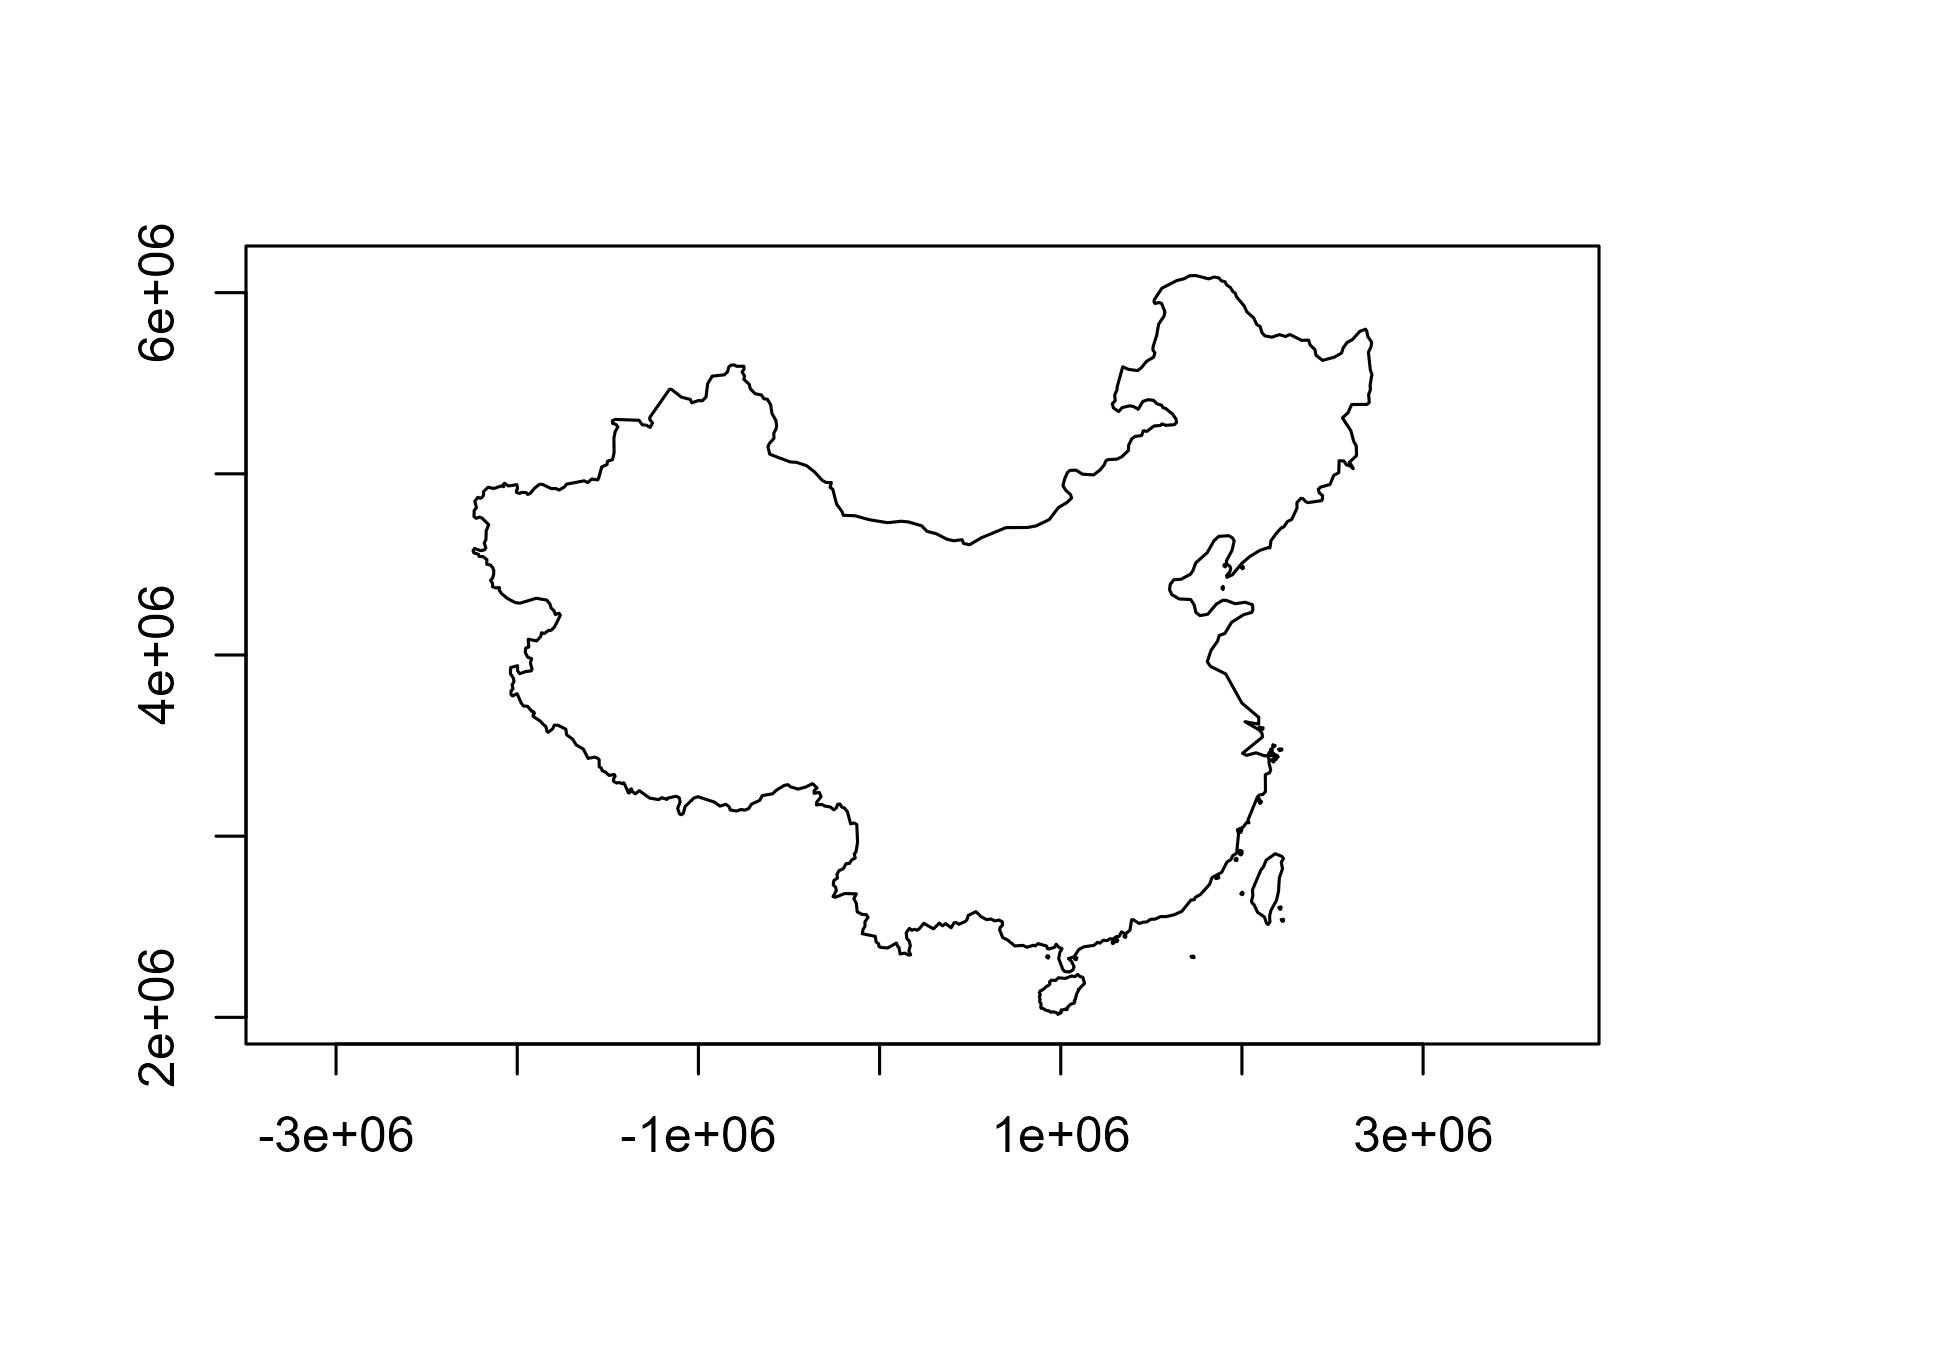
\includegraphics[width=0.6\linewidth]{_main_files/figure-latex/sugerencia-2} 

}

\caption{sf: Ejemplo de transformación usando crsuggest}\label{fig:sugerencia-2}
\end{figure}

\hypertarget{estaduxedstica-espacial}{%
\chapter{Estadística espacial}\label{estaduxedstica-espacial}}

La estadística espacial reconoce y aprovecha la ubicación espacial de los datos
a la hora de diseñar, recopilar, gestionar, analizar y mostrar las
observaciones. Éstas son generalmente \textbf{dependientes}, si bien existen modelos
espaciales a disposición del investigador que permiten tratar con dicha
dependencia espacial a la hora de llevar a cabo labores de predicción. Por
extensión, la estadística espacio-temporal incorpora, además, el tiempo y su
interacción con el espacio como argumento de ayuda en tales labores predictivas.

Las mediciones y modelos espaciales están presentes, sorprendentemente, en una
amplia variedad de disciplinas científicas. Los orígenes de la vida humana
vinculan los estudios de la evolución de las galaxias, la estructura de las
células biológicas y los patrones de asentamiento arqueológicos. Los ecologistas
estudian las interacciones entre plantas y animales. Silvicultores y
agricultores necesitan investigar las variaciones que se producen en el terreno
para sus experimentos. La estimación de las precipitaciones y de las reservas de
oro y petróleo es de vital importancia económica. Estos son, entre otros, buenos
ejemplos de la importancia del espacio (espacio-tiempo en su caso) en el mundo
de la Ciencia.

Sin embargo, el estudio de la \textbf{variabilidad espacial}, y sobre todo
espacio-temporal, es una disciplina relativamente nueva en el marco de la
Estadística, lo que explica la escasez de instrumentos de estadística espacial
30 años atrás. En los últimos 10 años ha habido una creciente toma de conciencia
de esta necesidad, habiéndose realizado un gran esfuerzo por buscar herramientas
adecuadas y útiles a tales efectos. Y todo ello porque utilizar modelos
espaciales o espacio-temporales para caracterizar y explotar la dependencia
espacial (o espacio-temporal) de un conjunto de observaciones tiene importantes
ventajas (\citet{montero_el_al_2011}):

\begin{enumerate}
\def\labelenumi{\arabic{enumi}.}
\item
  Modelos más generales, ya que, en la mayoría de los casos, los modelos
  clásicos que no tienen en consideración la dimensión espacial o la
  interacción de las dimensiones espacial y temporal son un caso particular de
  un modelo espacial o espacio-temporal.
\item
  Estimaciones más eficientes: de la tendencia, de los efectos de las
  variables explicativas, de promedios regionales,\ldots{}
\item
  Mejora de las predicciones: más eficientes, con propiedades de extrapolación
  más estables,\ldots{}
\item
  La variación espacial no explicada en la estructura de la media debe ser
  absorbida por la estructura del error, por lo que un modelo que incorpore la
  dependencia espacial puede decirse que está protegido frente a una mala
  especificación de este tipo. Esto, en muchos casos, tiene como resultado una
  simplificación en la especificación de la tendencia; en general, los modelos
  con dependencia espacial suelen tener una descripción más parsimoniosa (en
  ocasiones con muchos menos parámetros) que los clásicos modelos de
  superficie de tendencia.
\end{enumerate}

\hypertarget{antes-de-continuar-dependencia-espacial.}{%
\section{Antes de continuar\ldots{} dependencia espacial.}\label{antes-de-continuar-dependencia-espacial.}}

Frecuentemente los datos tienen una componente espacial y/o temporal asociada a
ellos y es de esperar que datos cercanos en el espacio o en el tiempo sean más
semejantes que aquellos que están más alejados; en cuyo caso \textbf{no} deben ser
modelados como estadísticamente independiente, sino que habrá que tomar en
cuenta esa dependencia espacial o espacio-temporal.

De forma natural y de acuerdo a la Ley Tobler (1973) surge la idea de que los
datos cercanos en el espacio o en el tiempo serán más similares y estarán más
correlacionados entres sí que aquellos que están más lejanos. Además, esta
correlación disminuye al aumentar la separación entre ellos, por lo que se puede
pensar en la presencia de una dependencia espacial o espacio-temporal. Esto da
lugar al concepto de proceso espacial o espacio-temporal.

Si los datos no exhiben dependencia espacial no tiene sentido aplicar las
herramientas de estadística espacial. Veamos un ejemplo simulado de unos datos
que muestras dependencia espacial y otros puramente aleatorios.

La Fig. \ref{fig:points-depiid} muestra unos datos simulados que presentan una
estructura de dependencia espacial (panel izquierdo) frente a unos datos
totalmente aleatorios (panel derecho), en ambos casos distribuidos de forma
irregular en el espacio.

\begin{figure}

{\centering 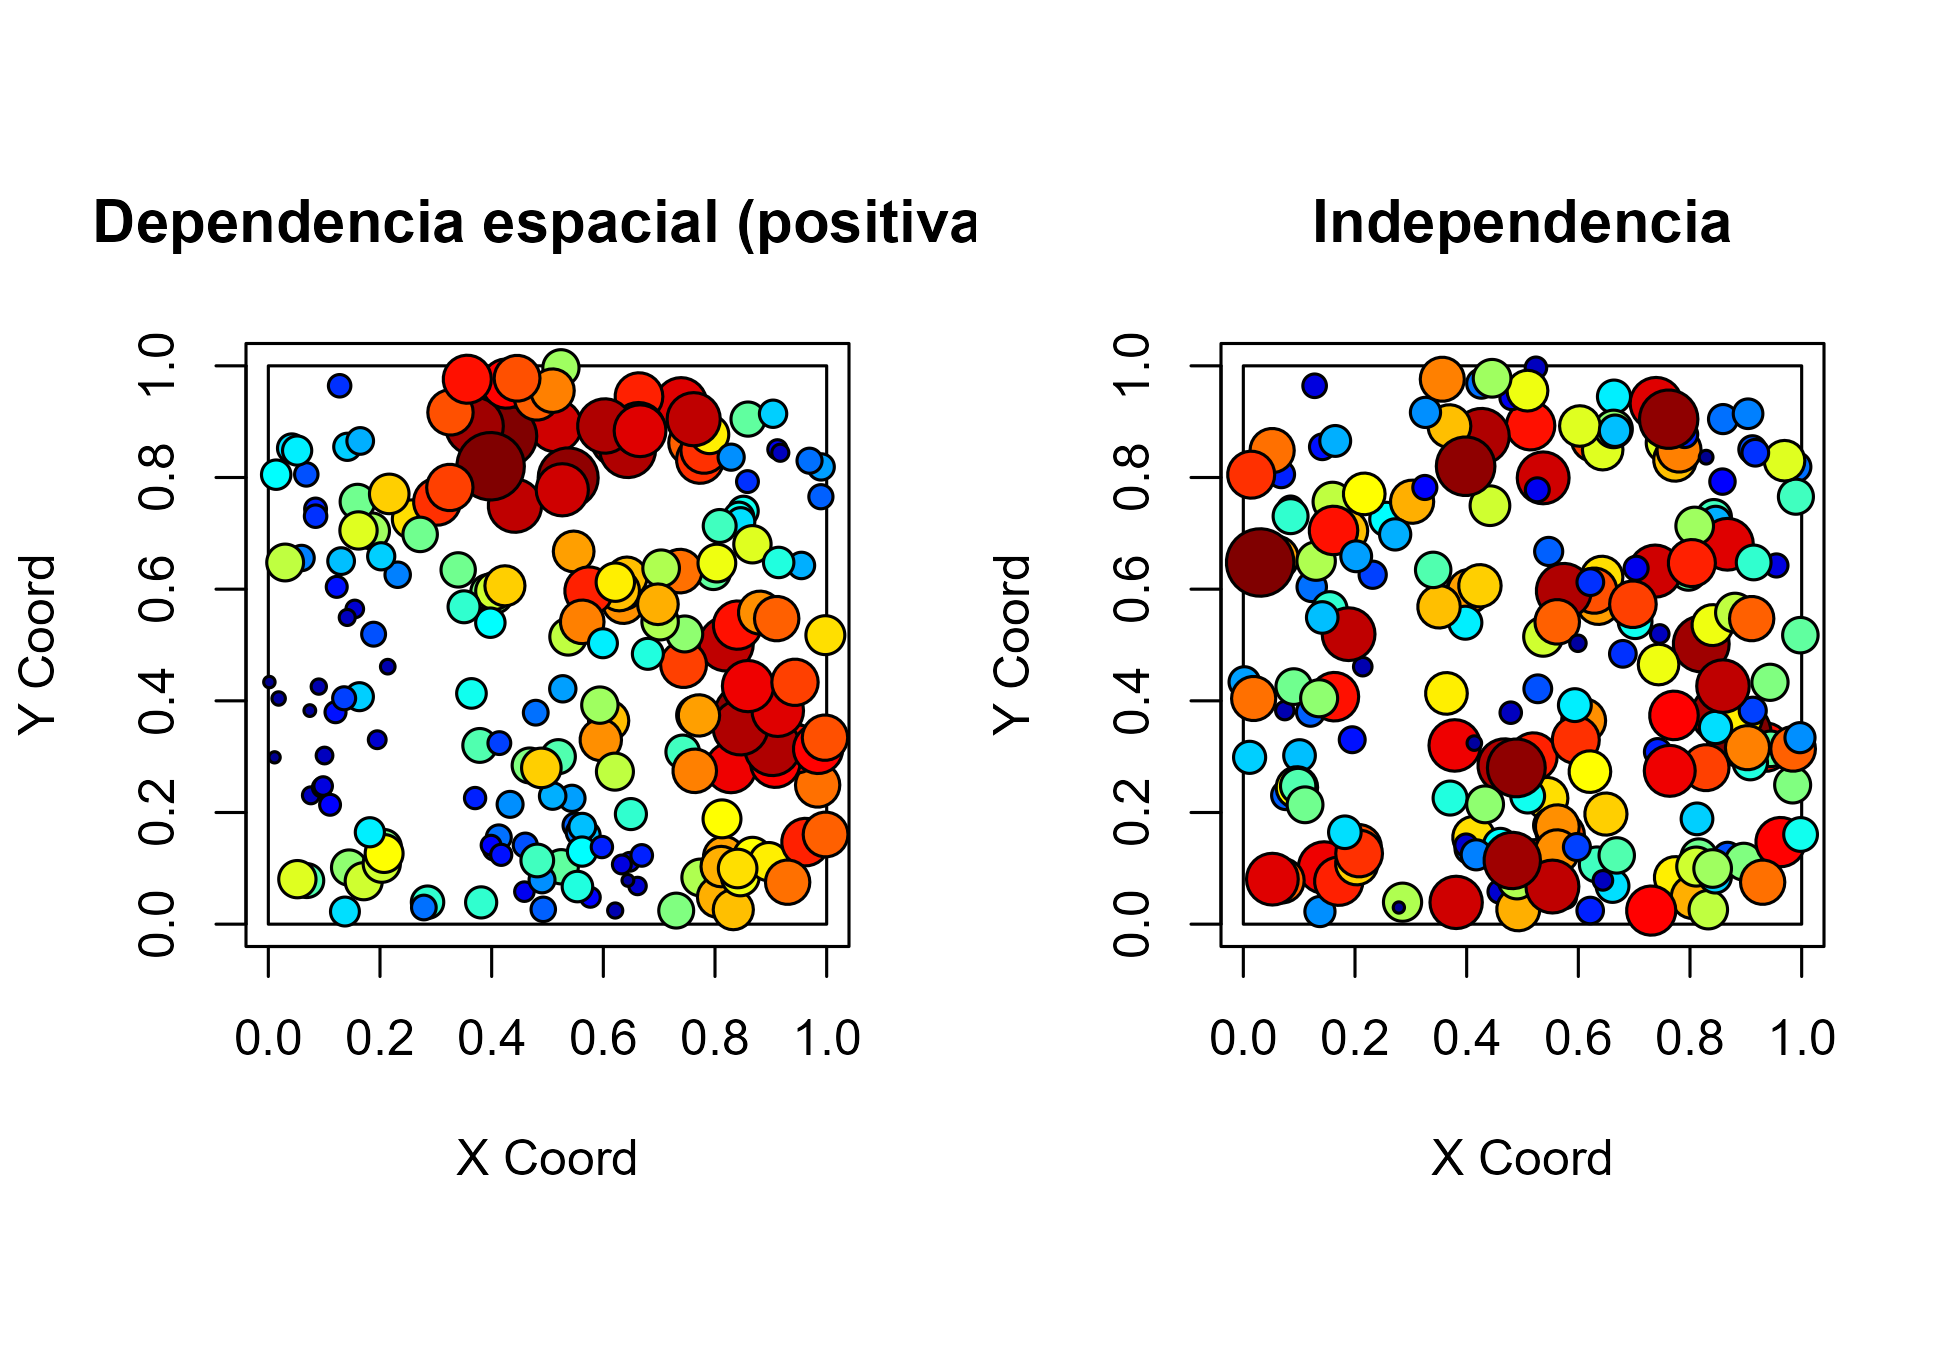
\includegraphics[width=0.6\linewidth]{_main_files/figure-latex/points-depiid-1} 

}

\caption{Puntos: Ejemplo de independencia espacial}\label{fig:points-depiid}
\end{figure}

La Fig. \ref{fig:lattice-dep-iid}, al igual que la Fig.
\ref{fig:points-depiid} presenta unos datos simulados donde que presentan una
estructura de dependencia espacial (panel izquierdo) frente a unos datos
totalmente aleatorios (panel derecho), pero en este caso estos datos se
distribuyen de forma ordenada en el espacio a través de una rejilla regular.

\begin{figure}

{\centering 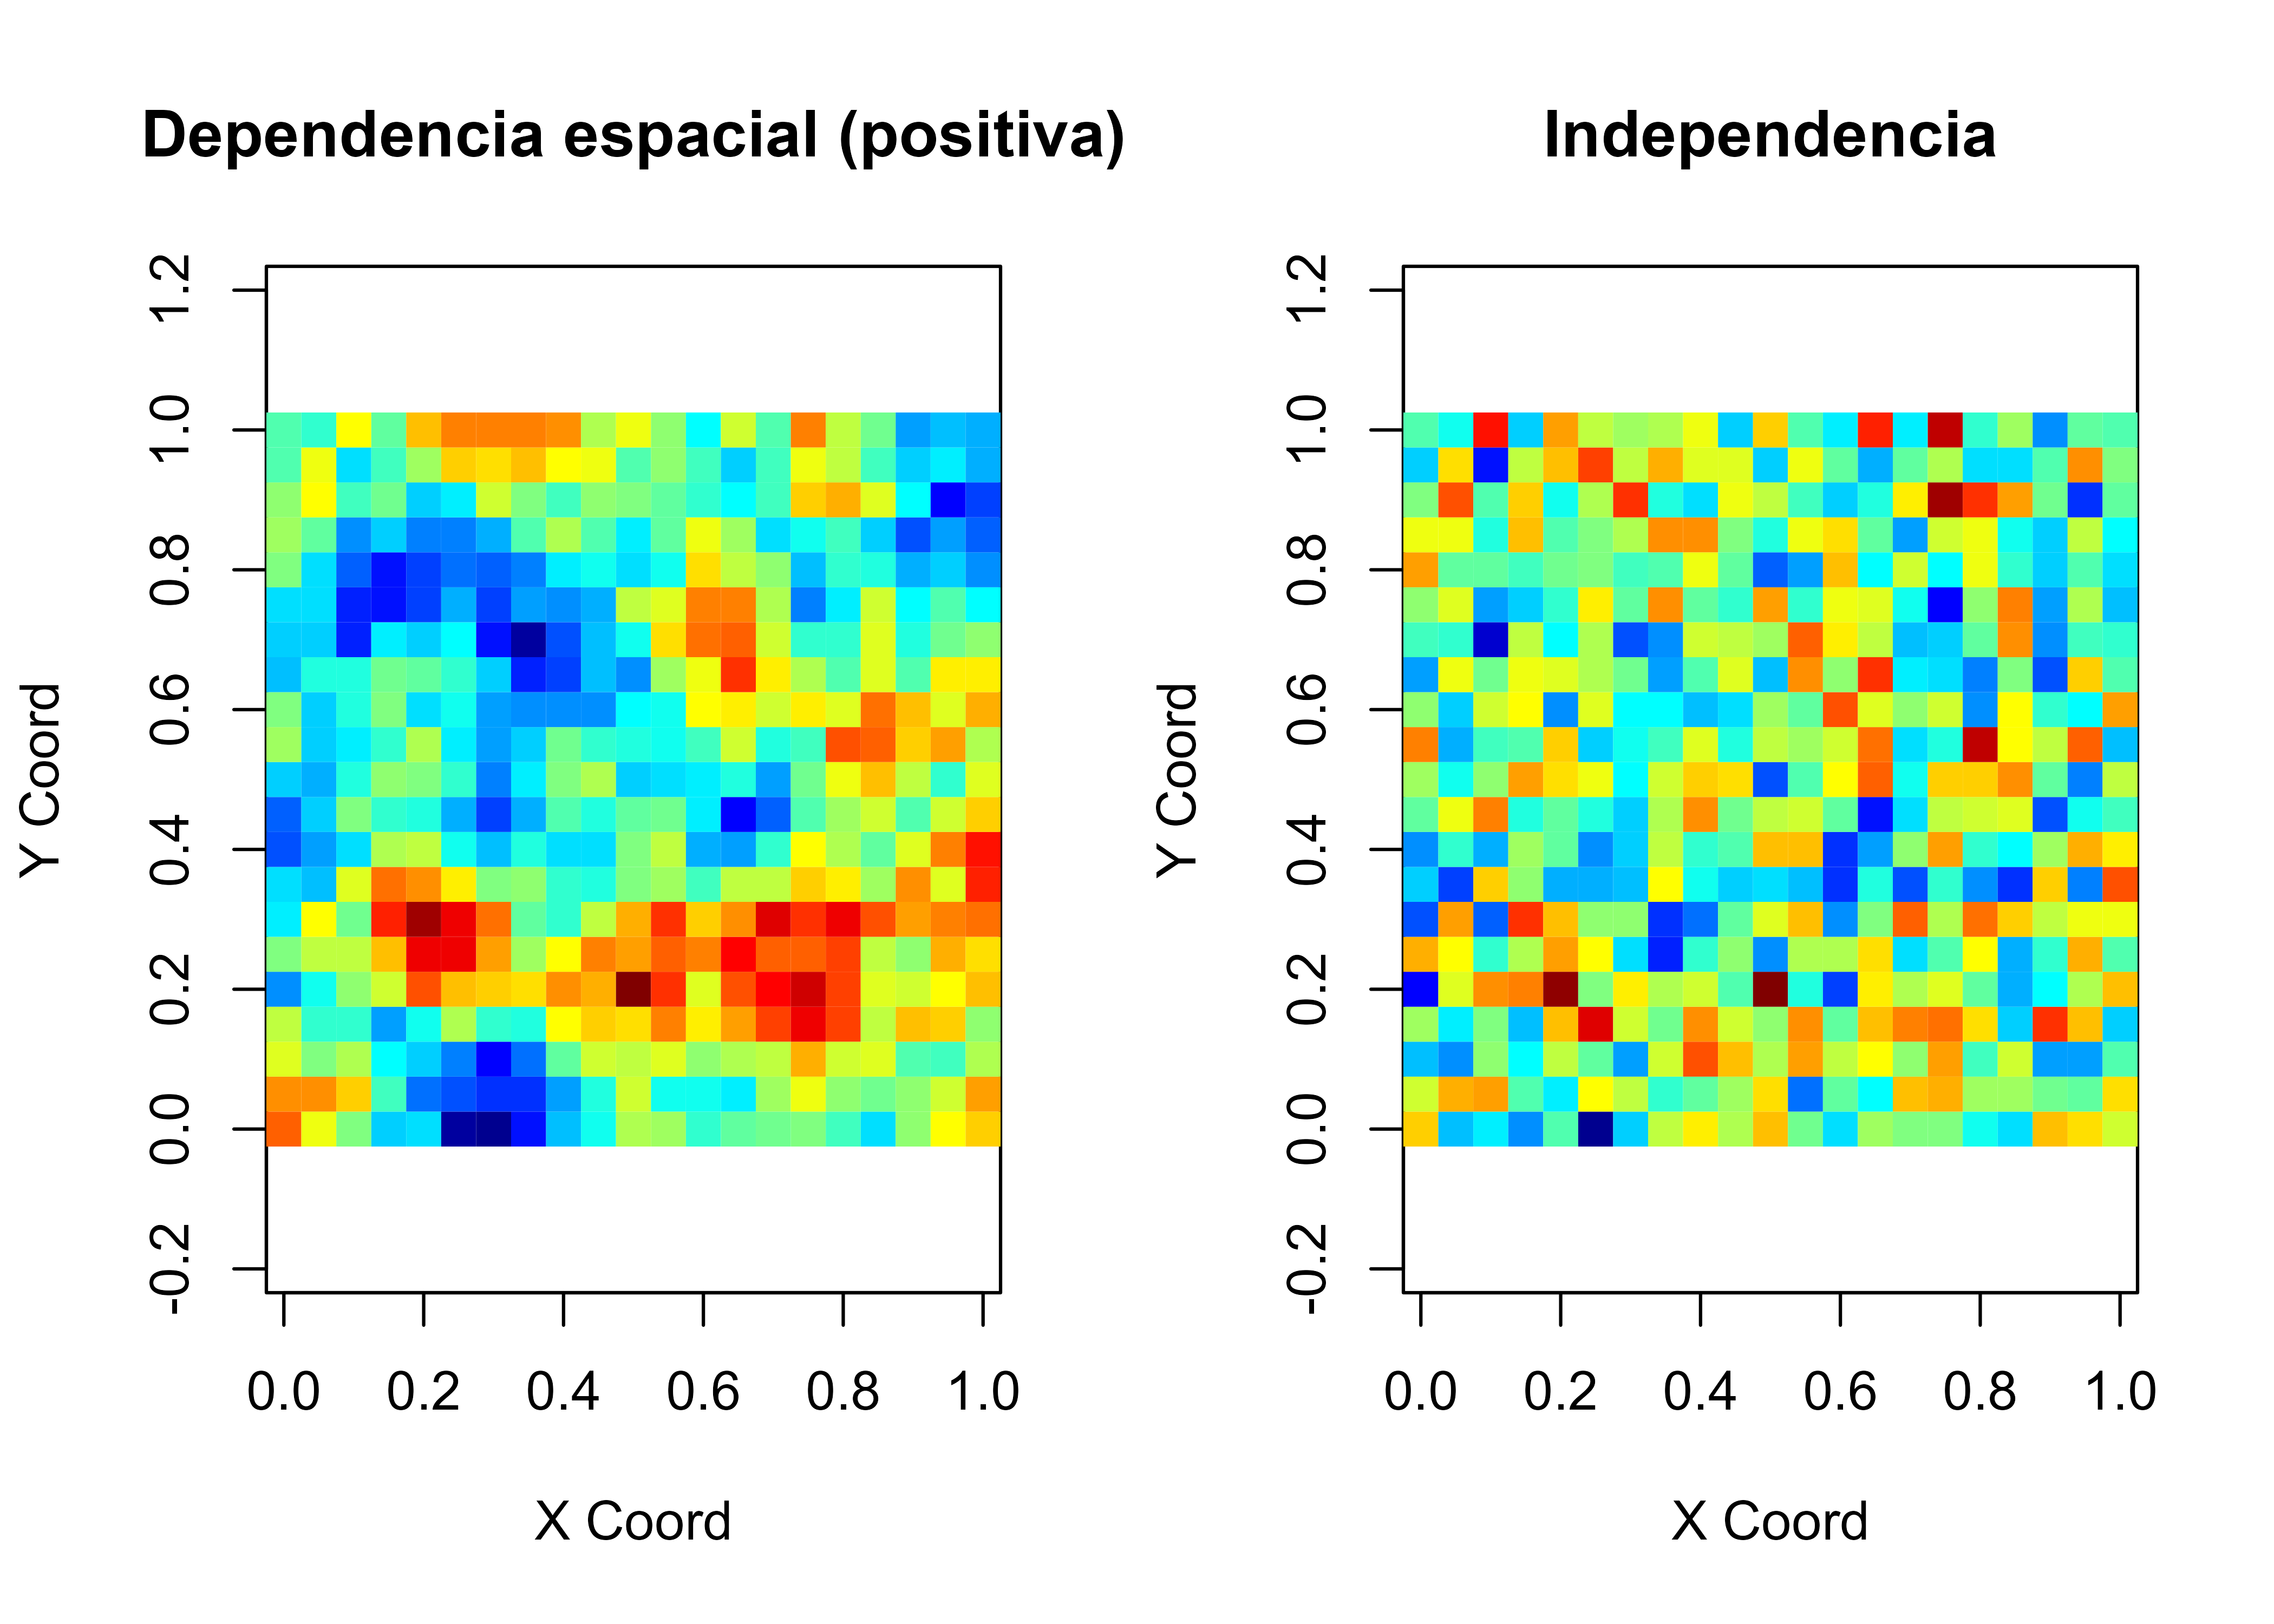
\includegraphics[width=0.6\linewidth]{_main_files/figure-latex/lattice-dep-iid-1} 

}

\caption{Rejilla: Ejemplo de independencia especial}\label{fig:lattice-dep-iid}
\end{figure}

\hypertarget{datos-espaciales}{%
\section{Datos espaciales}\label{datos-espaciales}}

Los \textbf{datos espaciales}, también conocidos como datos \textbf{geoespaciales}, son
aquellos datos relacionados o que contienen información de una localización o
área geográfica de la superficie de la Tierra.

La forma más intuitiva de representar los datos espaciales es a través de un
mapa.

\begin{Shaded}
\begin{Highlighting}[]
\CommentTok{\# Mapa de porcentaje de mujeres en Castilla{-}La Mancha}

\FunctionTok{library}\NormalTok{(mapSpain)}

\CommentTok{\# Datos de población}
\NormalTok{pob }\OtherTok{\textless{}{-}}\NormalTok{ mapSpain}\SpecialCharTok{::}\NormalTok{pobmun19}


\CommentTok{\# Datos en forma de tabla, sin información en formato espacial}
\CommentTok{\# head(pob)}

\CommentTok{\# Porcentaje}
\NormalTok{pob}\SpecialCharTok{$}\NormalTok{porc\_mujeres }\OtherTok{\textless{}{-}}\NormalTok{ pob}\SpecialCharTok{$}\NormalTok{women }\SpecialCharTok{/}\NormalTok{ pob}\SpecialCharTok{$}\NormalTok{pob19 }\SpecialCharTok{*} \DecValTok{100}

\CommentTok{\# Datos espaciales}
\NormalTok{geo }\OtherTok{\textless{}{-}} \FunctionTok{esp\_get\_munic}\NormalTok{(}\AttributeTok{region =} \StringTok{"Castilla{-}La Mancha"}\NormalTok{)}

\CommentTok{\# Estos datos tienen una columna (geometry) con coordenadas.}
\CommentTok{\# head(geo)}

\CommentTok{\# Une ambos datos}
\NormalTok{geo\_pob }\OtherTok{\textless{}{-}} \FunctionTok{merge}\NormalTok{(geo,}
\NormalTok{  pob,}
  \AttributeTok{by =} \FunctionTok{c}\NormalTok{(}\StringTok{"cpro"}\NormalTok{, }\StringTok{"cmun"}\NormalTok{),}
  \AttributeTok{all.x =} \ConstantTok{TRUE}
\NormalTok{)}

\CommentTok{\# Mapa básico}
\FunctionTok{plot}\NormalTok{(geo\_pob[}\StringTok{"porc\_mujeres"}\NormalTok{],}
  \CommentTok{\# Cambiamos titulo}
  \AttributeTok{main =} \StringTok{"Castilla{-}La Mancha: \% mujeres (2019)"}\NormalTok{,}

  \CommentTok{\# Cambiamos la paleta de colores para hacerlo mas atractivo}
  \CommentTok{\# border = NA,}
  \AttributeTok{pal =} \FunctionTok{hcl.colors}\NormalTok{(}\DecValTok{12}\NormalTok{, }\StringTok{"RdYlBu"}\NormalTok{)}
\NormalTok{)}
\end{Highlighting}
\end{Shaded}

\begin{figure}

{\centering 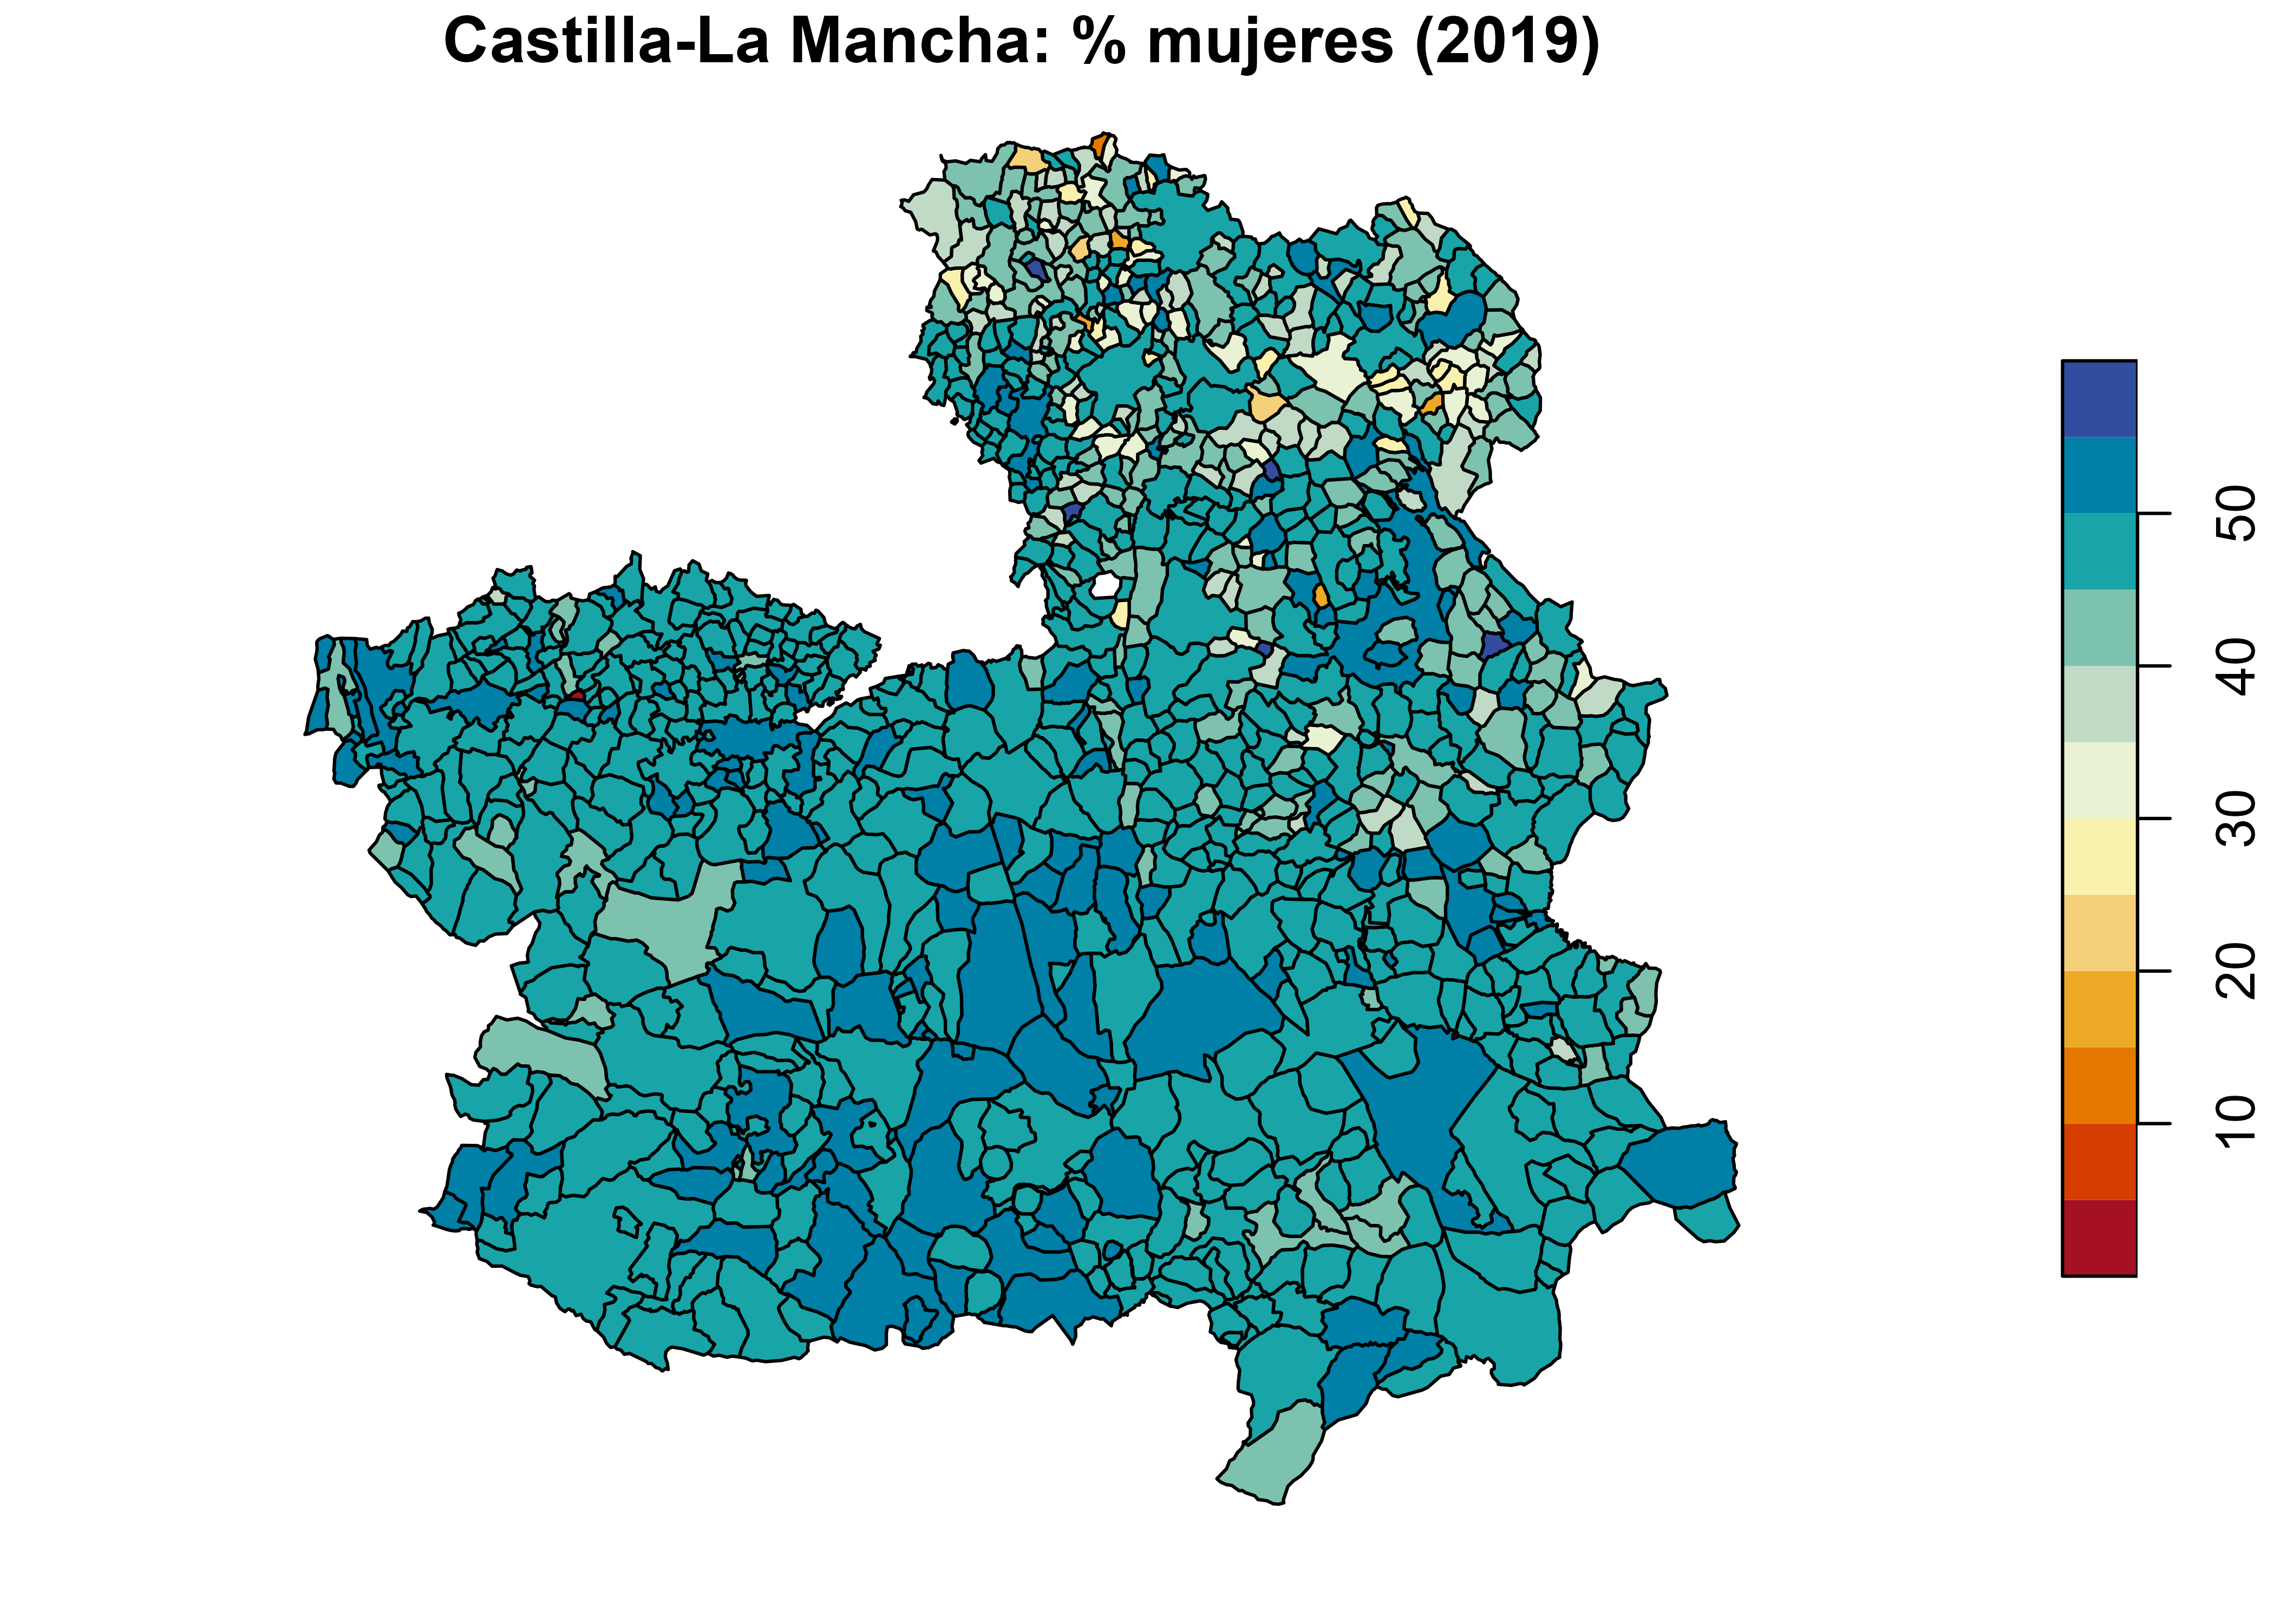
\includegraphics[width=0.6\linewidth]{_main_files/figure-latex/mapa-clm-1} 

}

\caption{Porcentaje de Mujeres en Castilla-La Mancha}\label{fig:mapa-clm}
\end{figure}

La Fig. \ref{fig:mapa-clm} presenta una serie de elementos gráficos,
característicos de los objetos espaciales:

\begin{itemize}
\item
  Los municipios de Castilla-la Mancha están representados por polígonos con
  un contorno negro y se rellenan de colores de acuerdo con la variable que
  estamos analizando, el porcentaje de mujeres en los municipios de
  Castilla-La Mancha en el año 2019.
\item
  Una leyenda explica el significado de los colores.
\item
  La variable, el porcentaje de mujeres en los municipios de Castilla-La
  Mancha en el año 2019, no parece distribuirse de manera independiente sino
  todo lo contrario, muestra un patrón espacial. Los municipios del las
  provincias Guadalajara y Cuenca (noreste) presentan tasas más bajas que los
  municipios del centro de la Comunidad.
\end{itemize}

\begin{Shaded}
\begin{Highlighting}[]
\FunctionTok{head}\NormalTok{(geo\_pob[}\StringTok{"porc\_mujeres"}\NormalTok{])}
\CommentTok{\#\textgreater{} Simple feature collection with 6 features and 1 field}
\CommentTok{\#\textgreater{} Geometry type: POLYGON}
\CommentTok{\#\textgreater{} Dimension:     XY}
\CommentTok{\#\textgreater{} Bounding box:  xmin: {-}2.18037 ymin: 38.5441 xmax: {-}1.31112 ymax: 39.35597}
\CommentTok{\#\textgreater{} Geodetic CRS:  ETRS89}
\CommentTok{\#\textgreater{}   porc\_mujeres                       geometry}
\CommentTok{\#\textgreater{} 1     52.02532 POLYGON (({-}1.58316 39.20446...}
\CommentTok{\#\textgreater{} 2     43.93064 POLYGON (({-}1.40607 39.12384...}
\CommentTok{\#\textgreater{} 3     51.14089 POLYGON (({-}2.0562 38.88697,...}
\CommentTok{\#\textgreater{} 4     48.55491 POLYGON (({-}1.54055 38.61066...}
\CommentTok{\#\textgreater{} 5     48.78419 POLYGON (({-}1.38514 39.35429...}
\CommentTok{\#\textgreater{} 6     44.49541 POLYGON (({-}2.15635 38.71074...}
\end{Highlighting}
\end{Shaded}

Antes de dibujar la Fig. \ref{fig:mapa-clm} tuvimos que leer los datos de la
librería \texttt{mapSpain} \citep{rmapspain} que contenía tanto la variable que hemos
analizado como el formato del mapa. Tras unir variable y mapa con la función
\texttt{merge()}. Al llevar a cabo un resumen del objeto espacial nos encontramos con
las siguiente información:

\begin{itemize}
\tightlist
\item
  el conjunto de datos (seleccionado) tiene 919 registros (municipios)
\item
  el tipo de geometría es POLYGON.
\item
  el CRS es ETRS89
\end{itemize}

\hypertarget{clasificaciuxf3n-de-datos-espaciales}{%
\section{Clasificación de datos espaciales}\label{clasificaciuxf3n-de-datos-espaciales}}

Tal y como acabamos de señalar y de acuerdo con Schabenberger y Gotway (2005, p.
6), debido a que los datos espaciales surgen en una gran variedad de campos y
aplicaciones, también hay una gran variedad de tipos de datos espaciales,
estructuras y escenarios. Por tanto, una clasificación exhaustiva de los datos
espaciales sería un reto muy difícil y hemos apostado por una clasificación
general, simple y útil de datos espaciales proporcionada por \citet{cressie1993}.

La \textbf{clasificación} de Cressie de datos espaciales se basa en la naturaleza del
dominio espacial en estudio. Dependiendo de esto, podemos tener: datos
geoestadísticos, datos de patrones de puntos y datos latice (véase Fig.
\ref{fig:hengl-cressie}, tomada de \href{http://spatial-analyst.net/book/system/files/Hengl_2009_GEOSTATe2c1w.pdf}{Hengl
(2009)}).

\begin{figure}

{\centering 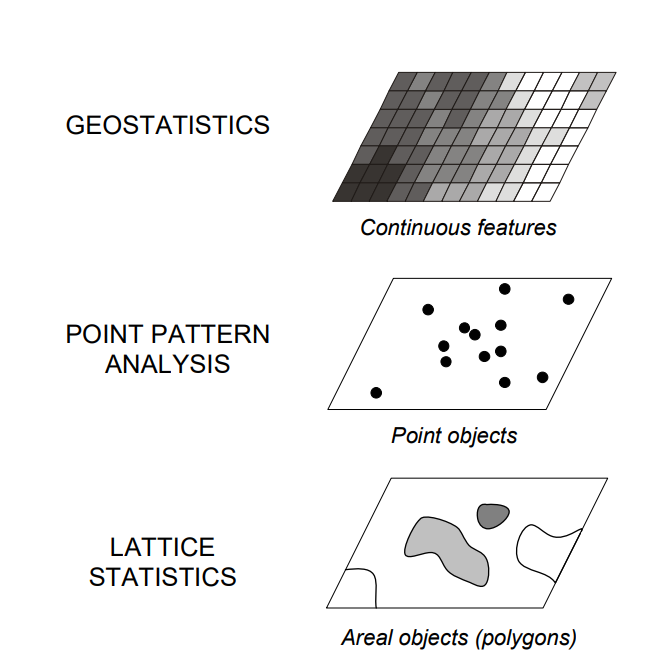
\includegraphics[width=0.6\linewidth]{img/hengl_cressie_clases} 

}

\caption{Clasificación de datos espaciales propuesta propuesta por @cressie1993}\label{fig:hengl-cressie}
\end{figure}

\textbf{GEMA: PUEDES REVISAR LA FORMULA?}

Siguiendo a \citet{cressie1993}, sea \(s ∈ ℝ\^d\) una localización en un espacio Euclideo
\(d-\)dimensional y \({Z(s)∶ s ∈ ℝ\^d}\) una función aleatoria espacial, donde \(Z\)
representa el atributo en el cual estamos interesados:

\begin{enumerate}
\def\labelenumi{\arabic{enumi}.}
\item
  \textbf{Datos geoestadísticos:} Surgen cuando el dominio de estudio es \textbf{continuo
  y fijo} \(D\). Es decir: (i) \(Z(s)\) se puede observar en cualquier punto del
  dominio (continuo); y (ii) los puntos en \(D\) no son estocásticos (son fijos,
  \(D\) es el mismo para todas las realizaciones de la función aleatoria
  espacial ).

  Algunos ejemplos de datos geoestadísticos son el nivel de un contaminante en
  una ciudad, los valores de precipitación o temperatura del aire en un país,
  las concentraciones de metales pesados en la capa superior del suelo de una
  región, etc.

  Es obvio que, al menos en teoría, el nivel de un contaminante específico
  podría medirse en cualquier lugar de la ciudad; Lo mismo puede decirse de
  las mediciones de precipitaciones o temperaturas del aire en un país o
  concentraciones de un metal pesado en una región. Sin embargo, en la
  práctica, no es posible una observación exhaustiva del proceso espacial. Por
  lo general, el proceso espacial se observa en un conjunto de ubicaciones
  (por ejemplo, el nivel de un contaminante específico en una ciudad se
  observa en los puntos donde están ubicadas las estaciones de monitoreo) y,
  basado en tales valores observados, el análisis geoestadístico reproduce el
  comportamiento de el proceso espacial en todo el dominio de interés.

  En el análisis geoestadístico lo más importante es cuantificar la
  correlación espacial entre observaciones (a través de la herramienta básica
  en geoestadística, el semivariograma) y utilizar esta información para
  lograr los objetivos anteriores.
\end{enumerate}

\begin{Shaded}
\begin{Highlighting}[]
\CommentTok{\# ejemplo cual??? tmin interpolado}
\end{Highlighting}
\end{Shaded}

\begin{enumerate}
\def\labelenumi{\arabic{enumi}.}
\setcounter{enumi}{1}
\item
  \textbf{Datos reticulares}: Surgen cuando: (i) el dominio bajo estudio \(D\) es
  \textbf{discreto}, es decir, \(Z(s)\) puede observarse en una serie de ubicaciones
  fijas que pueden enumerarse. Estas ubicaciones pueden ser puntos o regiones,
  pero generalmente son códigos postales, pistas censales, vecindarios,
  provincias, países, etc., y los datos en la mayoría de los casos son datos
  agregados espacialmente sobre estas áreas. Aunque estas regiones pueden
  tener una forma regular, normalmente la forma que tienen es irregular, y
  esto, junto con el carácter espacialmente agregado de la datos, es por lo
  que los datos latice tambien se denominan datos regionales. Y (ii) las
  ubicaciones en \(D\) no son estocásticas. Por supuesto, un concepto clave en
  el análisis de los datos lattice es el \textbf{vecindario} y la matriz \textbf{W}.

  Algunos ejemplos de reticulares incluyen la tasa de desempleo por estados,
  los datos de delincuencia por comarcas, rendimientos agrícolas en parcelas,
  precios medios de la vivienda por provincias, etc.
\end{enumerate}

\begin{Shaded}
\begin{Highlighting}[]
\CommentTok{\# ejemplo ¿¿ el de la renta??}
\end{Highlighting}
\end{Shaded}

\begin{enumerate}
\def\labelenumi{\arabic{enumi}.}
\setcounter{enumi}{2}
\item
  \textbf{Procesos de puntos:} Mientras que en los datos geoestadísticos y
  reticulares el dominio \(D\) es fijo, en los datos de patrones puntuales el
  dominio es discreto o continuo, pero \textbf{aleatorio}. Los patrones de puntos
  surgen cuando el atributo bajo estudio es la ubicación de los eventos
  (observaciones). Es decir, el interés radica en dónde ocurren eventos de
  interés.

  Algunos ejemplos de patrones de puntos son la ubicación de incendios en una
  región española, la ubicación de los árboles en un bosque o la ubicación de
  nidos en una colonia de aves reproductoras, la localización de los delitos
  en una ciudad, entre muchas otras.

  En estos En los casos, es obvio que D es aleatorio y los puntos de
  observación no dependen del investigador. El principal objetivo del análisis
  de patrones de puntos es determinar si la ubicación de los eventos tiende a
  exhibir un patrón sistemático sobre el área en estudio o, por el contrario,
  son aleatoriamente repartido.

  Más concretamente, nos interesa analizar si la ubicación de los eventos es
  completamente aleatorio espacialmente (la ubicación donde ocurren los
  eventos no se ve afectada por la ubicación de otros eventos), uniforme o
  regular (cada punto está tan lejos de todos sus vecinos como sea posible) o
  agrupados o agregados (la ubicación de los eventos se concentra en grupos).
\end{enumerate}

\begin{Shaded}
\begin{Highlighting}[]
\CommentTok{\# ejemplo, el de los accidentes??}
\end{Highlighting}
\end{Shaded}

\hypertarget{appendix-anexo}{%
\appendix}


\hypertarget{crsproy}{%
\chapter{Tipos de CRS proyectados}\label{crsproy}}

Existen varias familias de proyecciones, que se pueden clasificar de diversas
maneras: por tipo de superficie de proyección y por métrica a preservar.

\hypertarget{por-tipo-de-superficie-de-proyecciuxf3n}{%
\section{Por tipo de superficie de proyección}\label{por-tipo-de-superficie-de-proyecciuxf3n}}

El proceso de trasladar puntos de una esfera a un plano puede plantearse de
manera práctica como el ejercicio de envolver una esfera con una superificie
plana (como una hoja de papel) y trasladar los puntos de la esfera de manera
lineal al punto de la superficie plana más cercano a ella. La Fig.
\ref{fig:fi-proys} muestra estos tres tipos de proyección.

\begin{figure}

{\centering 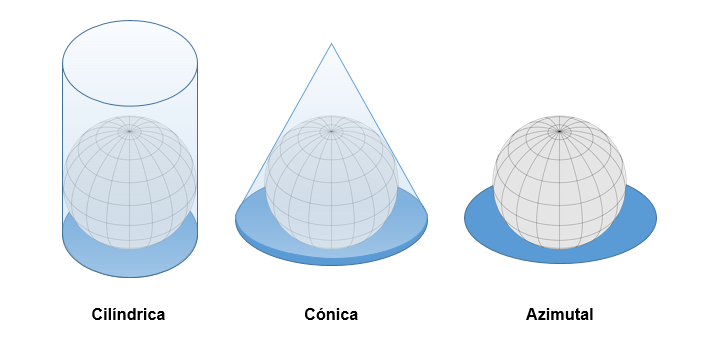
\includegraphics[width=0.6\linewidth]{img/tipos_proy} 

}

\caption{Tipos de proyección por superficie de proyección}\label{fig:fi-proys}
\end{figure}

A partir de este ejercicio, se plantean tres posibles soluciones (cilíndrica,
cónica y acimutal o planar), dependiendo del tipo de superficie que se use para
proyectar.

\begin{itemize}
\tightlist
\item
  \textbf{Proyecciones cilíndricas}: Son aquellas proyecciones donde la superficie
  de proyección conforma un cilindro alrededor de la Tierra. Una de las
  proyecciones cilíndricas más conocidas es la \textbf{proyección de Mercator} (Ver
  Fig. \ref{fig:mercator}).
\end{itemize}

\begin{figure}

{\centering 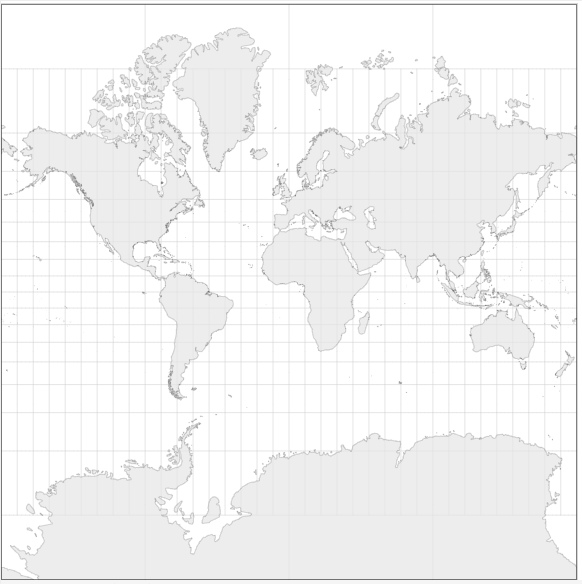
\includegraphics[width=0.4\linewidth]{img/mercator} 

}

\caption{Proyección Mercator}\label{fig:mercator}
\end{figure}

\begin{itemize}
\tightlist
\item
  \textbf{Proyecciones cónicas}: En este tipo de proyecciones, se plantea la
  superficie de proyección como una forma cónica. Como ejemplo, la
  \textbf{proyección cónica equiáreas de Albers} es una de las proyecciones que más
  suele usarse en la representación de mapas de América del Norte (Ver Fig.
  \ref{fig:albers}).
\end{itemize}

\begin{figure}

{\centering 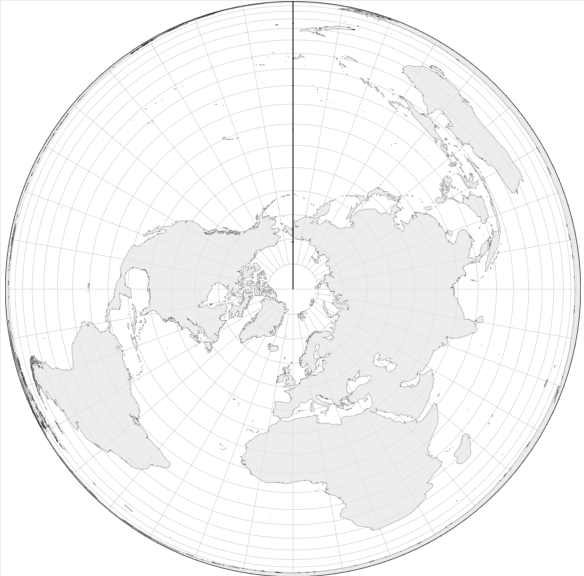
\includegraphics[width=0.4\linewidth]{img/albers_conic} 

}

\caption{Proyección cónica equiáreas de Albers}\label{fig:albers}
\end{figure}

\begin{itemize}
\tightlist
\item
  \textbf{Proyecciones acimutales o planares:} En este tipo de proyección se
  proyecta una porción de la Tierra sobre un plano que es tangente a la misma
  en el punto de referencia. Como ejemplos de proyecciones acimutales podemos
  destacar la \textbf{proyección ortográfica} (Ver Fig. \ref{fig:orto}).
\end{itemize}

\begin{figure}

{\centering 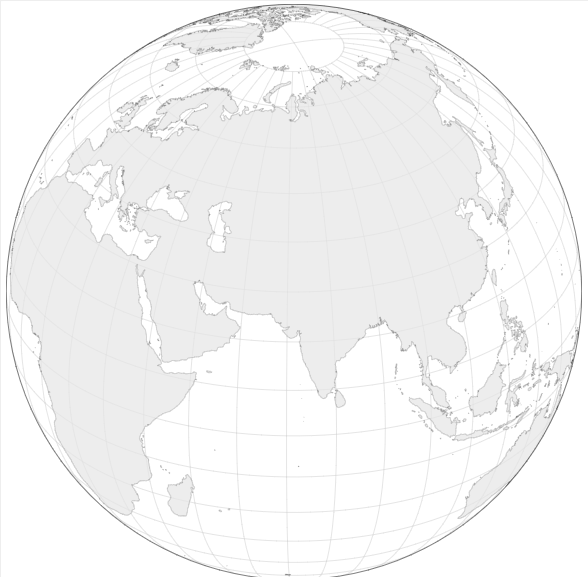
\includegraphics[width=0.4\linewidth]{img/orto} 

}

\caption{Proyección ortogonal}\label{fig:orto}
\end{figure}

\hypertarget{por-muxe9trica-a-preservar}{%
\section{Por métrica a preservar}\label{por-muxe9trica-a-preservar}}

Es importante tener en cuenta que cualquier proyección de la superficie de la
Tierra produce distorsiones en una o varias características geográficas. Como
ejemplo clásico, la proyección de Mercator produce distorsiones del \textbf{tamaño}
especialmente en aquellas regiones más cercanas a los polos (Groenlandia, que la
proyección de Mercator presenta una área similar a la de África, tiene menor
superficie real que Argelia). Otras de las métricas que suele verse
distorsionada son la \textbf{distancia} entre dos puntos geográficos, la
\textbf{dirección} o la \textbf{forma} de regiones de la Tierra.

A lo largo de la Historia se han desarrollado diversas proyecciones cuyo
objetivo es preservar alguna o varias de las propiedades mencionadas
anteriormente, sin embargo es importante destacar que \textbf{no existe una proyección
que sea capaz de preservar todas las métricas a la vez}.

Según la metrica a presevar, las proyecciones se pueden clasificar en:

\begin{itemize}
\tightlist
\item
  \textbf{Proyecciones conformales:} Intentan preservar los \textbf{ángulos} que se
  forman en la superficie terrestre. Por ejemplo, la proyección de Mercator
  representa ángulos rectos en las intersecciones de los paralelos y los
  meridianos (Ver Fig. \ref{fig:conform}).
\end{itemize}

\begin{figure}

{\centering 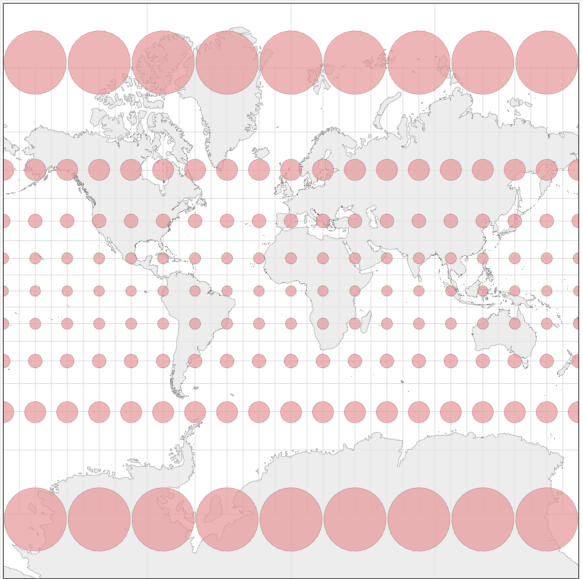
\includegraphics[width=0.3\linewidth]{img/conform} 

}

\caption{Ejemplo de proyección conformal: Mercator}\label{fig:conform}
\end{figure}

\begin{itemize}
\tightlist
\item
  \textbf{Proyecciones equivalentes}: Preservan las proporciones de las \textbf{áreas},
  provocando a su vez deformaciones en el resto de características, como la
  forma o los ángulos. La proyección acimutal equivalente de Lambers es un
  tipo de proyección equivalente (Ver Fig. \ref{fig:equiv}).
\end{itemize}

\begin{figure}

{\centering 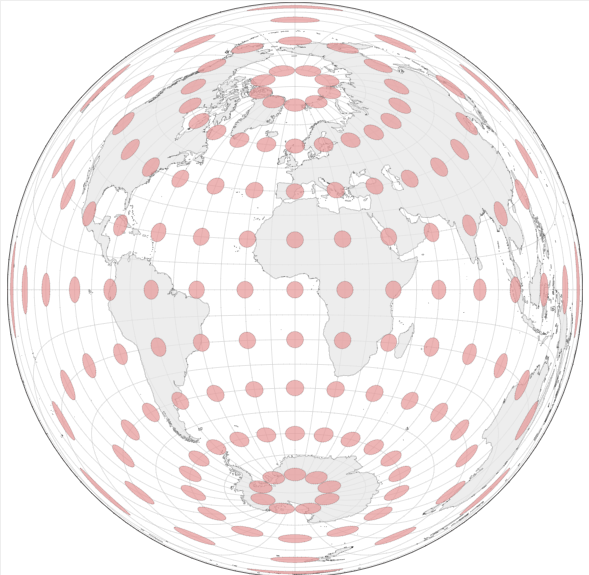
\includegraphics[width=0.3\linewidth]{img/equiv} 

}

\caption{Ejemplo de proyección equivalente: Proyección acimutal equivalente de Lambers}\label{fig:equiv}
\end{figure}

\begin{itemize}
\tightlist
\item
  \textbf{Proyecciones equidistantes:} Preservan la \textbf{distancia} entre dos puntos
  geográficos específicos. Por ejemplo, la proyección Plate carré preserva la
  distancia entre el Polo Norte y el Polo Sur (Ver Fig. \ref{fig:equidist}).
\end{itemize}

\begin{figure}

{\centering 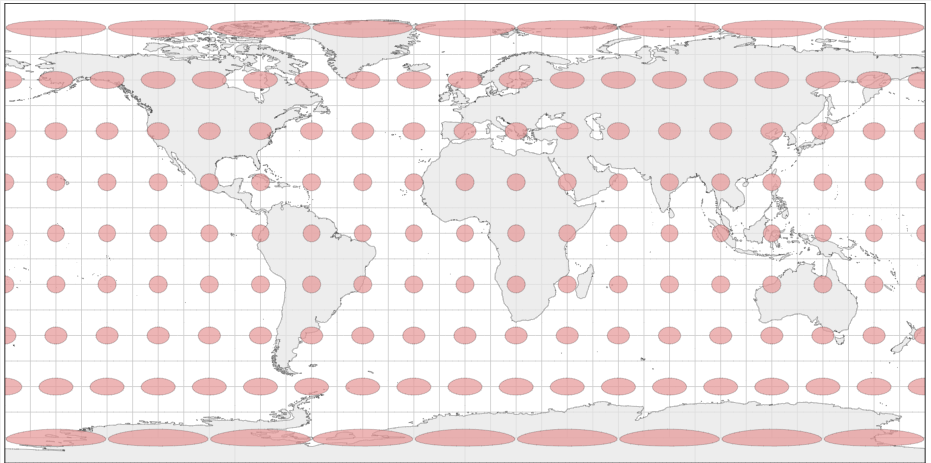
\includegraphics[width=0.3\linewidth]{img/equidist} 

}

\caption{Ejemplo de proyección equidistante: Platé carre}\label{fig:equidist}
\end{figure}

\begin{itemize}
\tightlist
\item
  \textbf{Proyecciones de compromiso}: No intentan preservar ninguna métrica en
  concreto. En su lugar, se centran en intentar encontrar un \textbf{equilibrio}
  entre las diversas distorsiones que provocan para intentar dar una
  representación más o menos representativa de la superficie terrestre. La
  proyección de Winkel Tripel, usada en los mapas de National Geographic, es
  un ejemplo de proyección de compromiso (Ver Fig. \ref{fig:comp}).
\end{itemize}

\begin{figure}

{\centering 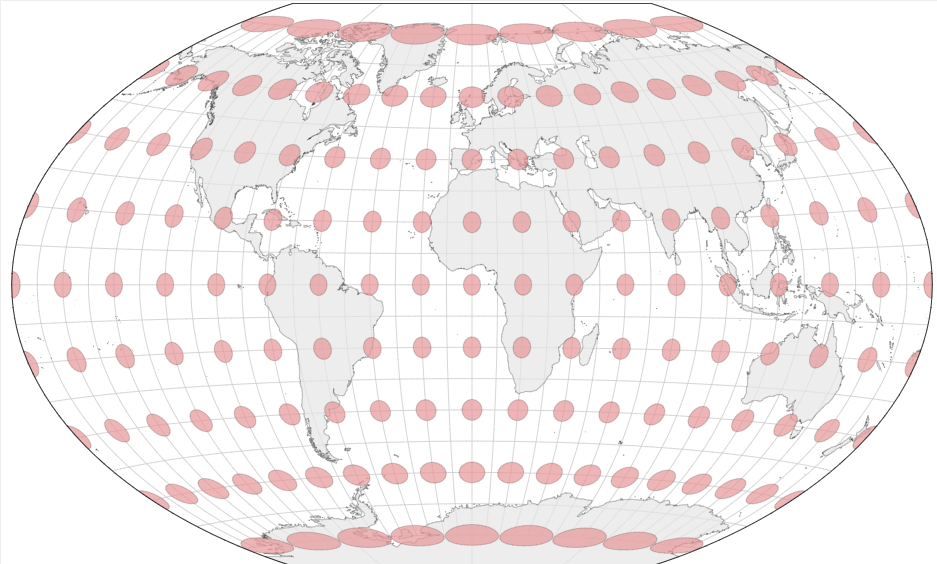
\includegraphics[width=0.3\linewidth]{img/comp} 

}

\caption{Ejemplo de proyección de compromiso: Winkel Tripel}\label{fig:comp}
\end{figure}

En los anteriores ejemplos se ha añadido a cada proyección la \textbf{indicatriz de
Tissot}. Ésta consiste en una serie de círculos imaginarios de igual área
distribuidos sobre la superficie esférica de la Tierra en determinados puntos.
De este manera, al presentar la indicatriz de Tissot en una proyección
específica, se puede entender de una manera intuitiva la distorsión provocada
por dicha proyección, ya que los círculos se ven distorsionados o preservados
según los parámetros y la naturaleza de la proyección en cuestión.

  \bibliography{book.bib}

\end{document}
